%%
%% Copyright (c) 2018-2019 Weitian LI <liweitianux@sjtu.edu.cn>
%% Creative Commons BY 4.0
%%

% Class options:
%   bachelor|master|doctor	% 必选项
%   fontset=fandol|adobe|windows
%   oneside|twoside
%   openany|openright
%   zihao=-4|5			% 正文字号: 小四、五号(默认)
%   english			% 启用英文模版
%   review			% 盲审论文,隐去作者姓名、学号、
%				% 导师姓名、致谢、发表论文和参与的项目
%   submit			% 定稿提交的论文,插入签名扫描版的
%				% 原创性声明、授权声明
\documentclass[
  doctor,
  openright,
  twoside,
  %review,
]{sjtuthesis}

\usepackage{microtype}
\usepackage{fontawesome5}

\defaultfontfeatures{Mapping=tex-text}
\setmainfont{Source Serif Pro}
\setsansfont{Source Sans Pro}
\setmonofont{Source Code Pro}
\setmathfont{Asana Math}

\setCJKmainfont{Source Han Serif SC}
\setCJKsansfont{FandolKai}
\setCJKmonofont{FandolFang}
\xeCJKsetup{PunctStyle=kaiming}

\graphicspath{{./}{figures/}{figures/self/}}

% biblatex
% Credit: http://www.khirevich.com/latex/biblatex/
\ExecuteBibliographyOptions{
  backref=true,
  mincitenames=1,
  maxcitenames=2,
}
% period after the authors
\renewcommand{\labelnamepunct}{\addperiod\space}
% discard the period at the very end of a record
\renewcommand{\finentrypunct}{}
% discard the period after the doi link
\renewcommand{\newunitpunct}{\addspace\midsentence}
% use lowercase English for backref
\DefineBibliographyStrings{english}{%
  backrefpage  = {\lowercase{s}ee p.}, % for single page number
  backrefpages = {\lowercase{s}ee pp.} % for multiple page numbers
}
\DeclareDelimFormat{finalnamedelim}{\addspace\&\space}
\DeclareFieldFormat[book]{title}{\textbf{#1}\addperiod\space}
\DeclareFieldFormat[article,inproceedings]{title}{\textit{#1}\addperiod\space}
\DeclareFieldFormat[inproceedings]{booktitle}{\textit{#1}\addperiod\space}
\DeclareFieldFormat[article,inproceedings]{volume}{\textbf{#1}\addcolon\space}
\DeclareFieldFormat{pages}{#1\addperiod\space}
%
\newcommand{\citeay}[1]{\citeauthor{#1} \citeyear{#1} \parencite{#1}}
\newcommand{\citet}[1]{\citeauthor{#1} (\citeyear{#1})\cite{#1}}

% Change 'emph' style to bold face
\let\emph\relax  % there's no \RedeclareTextFontCommand
\DeclareTextFontCommand{\emph}{\boldmath\bfseries}

% Use sans-serif for URLs by '\url'
\urlstyle{sf}

% Continuous footnote numbering
\counterwithout{footnote}{chapter}

% Set labels for hyperref's '\autoref'
% Credit: https://tex.stackexchange.com/a/66150
\def\equationautorefname~#1\null{式~(#1)\null}
\def\chapterautorefname~#1\null{第{#1}章\null}
\def\sectionautorefname{\textsection}
\def\subsectionautorefname{\textsection}
\def\figureautorefname{图}
\def\tableautorefname{表}

% Custom commands
\newcommand{\doi}[1]{\href{https://doi.org/#1}{\textsc{doi}:#1}}
\newcommand{\ads}[1]{\href{http://adsabs.harvard.edu/abs/#1}{\textsc{ads}:#1}}
\newcommand{\arxiv}[1]{\href{https://arixv.org/abs/#1}{\textsc{arXiv}:#1}}
\newcommand{\email}[1]{\href{mailto:#1}{\texttt{#1}}}
\newcommand{\circled}[1]{{\large\textcircled{\small #1}}}
\newcommand{\Cpi}{\symup{\pi}}  % constant pi
\newcommand{\Ce}{\symup{e}}  % constant e
\newcommand{\Ci}{\symup{i}}  % complex i
\newcommand{\R}[1]{\mathrm{#1}}  % text math alphabets
\newcommand{\B}[1]{\symbf{#1}}  % single-letter bold math
\newcommand{\V}[1]{\symbfit{#1}}  % bold italic
\newcommand{\M}[1]{\symbfsf{#1}}  % bold sans-serif (matrix)
\newcommand{\D}[1]{\mathrm{d}#1}
\newcommand{\diff}[2]{\frac{\mathrm{d}#1}{\mathrm{d}#2}}
\newcommand{\pdiff}[2]{\frac{\partial #1}{\partial #2}}
\newcommand{\klos}{\text{$k_{\parallel}$}}
\newcommand{\kperp}{\text{$k_{\bot}$}}
%
\def\lcdm/{$\Lambda$CDM}
\def\Hi/{H\textsc{i}}
\def\Hii/{H\textsc{ii}}

% Journals
\newcommand\aap{Astronomy and Astrophysics}
\newcommand\aapr{Astronomy and Astrophysics Review}
\newcommand\aaps{Astronomy and Astrophysics Supplement Series}
\newcommand\aj{Astronomical Journal}
\newcommand\ao{Applied Optics}
\newcommand\aplett{Astrophysics Letters}
\newcommand\apj{Astrophysical Journal}
\newcommand\apjl{Astrophysical Journal Letters}
\newcommand\apjs{Astrophysical Journal Supplement Series}
\newcommand\apss{Astrophysics and Space Science}
\newcommand\araa{Annual Review of Astronomy and Astrophysics}
\newcommand\arep{Astronomy Reports}
\newcommand\aspc{ASP Conference Series}
\newcommand\baas{Bulletin of the American Astronomical Society}
\newcommand\caa{Chinese Astronomy and Astrophysics}
\newcommand\cjaa{Chinese Journal of Astronomy and Astrophysics}
\newcommand\fcp{Fundamentals of Cosmic Physics}
\newcommand\grl{Geophysics Research Letters}
\newcommand\iaucirc{IAU Cirulars}
\newcommand\icarus{Icarus}
\newcommand\japa{Journal of Astrophysics and Astronomy}
\newcommand\jcap{Journal of Cosmology and Astroparticle Physics}
\newcommand\jcp{Journal of Chemical Physics}
\newcommand\jgr{Journal of Geophysics Research}
\newcommand\jqsrt{Journal of Quantitiative Spectroscopy and Radiative Transfer}
\newcommand\jrasc{Journal of the RAS of Canada}
\newcommand\memras{Memoirs of the RAS}
\newcommand\memsai{Memoire della Societa Astronomica Italiana}
\newcommand\mnassa{Monthly Notes of the Astronomical Society of Southern Africa}
\newcommand\mnras{Monthly Notices of the Royal Astronomical Society}
\newcommand\na{New Astronomy}
\newcommand\nar{New Astronomy Review}
\newcommand\nat{Nature}
\newcommand\nphysa{Nuclear Physics A}
\newcommand\pra{Physical Review A: General Physics}
\newcommand\prb{Physical Review B: Solid State}
\newcommand\prc{Physical Review C}
\newcommand\prd{Physical Review D}
\newcommand\pre{Physical Review E}
\newcommand\prl{Physical Review Letters}
\newcommand\pasa{Publications of the Astronomical Society of Australia}
\newcommand\pasp{Publications of the Astronomical Society of the Pacific}
\newcommand\pasj{Publications of the Astronomical Society of Japan}
\newcommand\physrep{Physics Reports}
\newcommand\planss{Planetary Space Science}
\newcommand\procspie{Proceedings of the Society of Photo-Optical Instrumentation Engineers}
\newcommand\qjras{Quarterly Journal of the RAS}
\newcommand\sci{Science}
\newcommand\skytel{Sky and Telescope}
\newcommand\solphys{Solar Physics}
\newcommand\ssr{Space Science Reviews}

% New math operators
\DeclareMathOperator{\erf}{erf}
\DeclareMathOperator{\sinc}{sinc}

% siunitx settings and new units
\sisetup{
  range-phrase=\text{--},
  range-units=single,
  product-units=repeat,
  list-separator={, },
  list-final-separator={, and },
  separate-uncertainty=true,
}
%
\DeclareSIUnit\arcsec{arcsec}
\DeclareSIUnit\arcmin{arcmin}
\DeclareSIUnit\cMpc{cMpc}  % comoving Mpc
\DeclareSIUnit\cGpc{cGpc}  % comoving Gpc
\DeclareSIUnit\deg{deg}
\DeclareSIUnit\dyne{dyn}
\DeclareSIUnit\erg{erg}
\DeclareSIUnit\esu{esu}
\DeclareSIUnit\franklin{Fr}
\DeclareSIUnit\gauss{G}
\DeclareSIUnit\hubble{\ensuremath{\mathit{h}}}
\DeclareSIUnit\jansky{Jy}
\DeclareSIUnit\lightyear{ly}
\DeclareSIUnit\parsec{pc}
\DeclareSIUnit\rayleigh{Rayleigh}
\DeclareSIUnit\solarmass{\ensuremath{\mathrm{M}_{\odot}}}
\DeclareSIUnit\statcoulomb{statC}
\DeclareSIUnit\year{yr}
%
\DeclareSIUnit\kpc{\kilo\parsec}
\DeclareSIUnit\mJy{\milli\jansky}
\DeclareSIUnit\mK{\milli\kelvin}
\DeclareSIUnit\Gpc{\giga\parsec}
\DeclareSIUnit\Gyr{\giga\year}
\DeclareSIUnit\Mpc{\mega\parsec}
\DeclareSIUnit\Myr{\mega\year}
\DeclareSIUnit\uG{\micro\gauss}

\usepackage{acro}  % acronyms, symbols, glossaries
\acsetup{
  list-heading=chapter,
  extra-style=bracket,
  extra-format={\it},
}
%%
%% Copyright (c) 2018 Weitian LI <liweitianux@sjtu.edu.cn>
%% Creative Commons BY 4.0
%%

\DeclareAcronym{DA}{
  short = \ensuremath{D_{\!A}},
  long = 角直径距离,
  foreign = angular diameter distance,
  class = symbol,
}

\DeclareAcronym{DL}{
  short = \ensuremath{D_{\!L}},
  long = 光度距离,
  foreign = luminosity distance,
  class = symbol,
}

\DeclareAcronym{DM}{
  short = \ensuremath{D_{\!M}},
  long = 横向共动距离,
  foreign = transverse comoving distance,
  class = symbol,
}

\DeclareAcronym{Dz}{
  short = \ensuremath{D(z)},
  long = 增长因子,
  foreign = growth factor,
  class = symbol,
}

\DeclareAcronym{delta-crit}{
  short = \ensuremath{\delta_c(z)},
  long = 临界线性过密度,
  foreign = critical linear overdensity,
  class = symbol,
}

\DeclareAcronym{Delta-vir}{
  short = \ensuremath{\Delta_{\R{vir}}(z)},
  long = 星系团的平均过密度,
  foreign = average overdensity,
  class = symbol,
}

\DeclareAcronym{Ez}{
  short = \ensuremath{E(z)},
  long = 红移演化因子,
  class = symbol,
}

\DeclareAcronym{G}{
  short = \ensuremath{G},
  long = 引力常数,
  class = symbol,
}

\DeclareAcronym{h}{
  short = \si{\hubble},
  long = 无量纲 Hubble 常数,
  class = symbol,
}

\DeclareAcronym{H0}{
  short = \ensuremath{H_0},
  long = 当前的 Hubble 常数,
  class = symbol,
}

\DeclareAcronym{Hz}{
  short = \ensuremath{H(z)},
  long = 红移为 $z$ 时的 Hubble 常数,
  class = symbol,
}

\DeclareAcronym{L-bolo}{
  short = \ensuremath{L_{\R{bolo}}},
  long = 热光度,
  foreign = bolometric luminosity,
  class = symbol,
}

\DeclareAcronym{M-vir}{
  short = \ensuremath{M_{\R{vir}}},
  long = 维里质量,
  foreign = virial mass,
  class = symbol,
}

\DeclareAcronym{ns}{
  short = \ensuremath{n_s},
  long = 原初扰动的标量谱指数,
  foreign = scalar spectral index,
  class = symbol,
}

\DeclareAcronym{Ob0}{
  short = \ensuremath{\Omega_b},
  long = 当前的宇宙重子物质密度参数,
  sort = Omega-b,
  class = symbol,
}

\DeclareAcronym{Ofz}{
  short = \ensuremath{\Omega_f(z)},
  long = 红移为 $z$ 时的宇宙物质比例,
  sort = Omega-f-z,
  class = symbol,
}

\DeclareAcronym{Om0}{
  short = \ensuremath{\Omega_m},
  long = 当前的宇宙物质(包括重子物质和暗物质)密度参数,
  sort = Omega-m,
  class = symbol,
}

\DeclareAcronym{Ol0}{
  short = \ensuremath{\Omega_{\Lambda}},
  long = 当前的宇宙常数或真空能密度参数,
  sort = Omega-Lambda,
  class = symbol,
}

\DeclareAcronym{r-vir}{
  short = \ensuremath{r_{\R{vir}}},
  long = 维里半径,
  foreign = virial radius,
  class = symbol,
}

\DeclareAcronym{rho-crit}{
  short = \ensuremath{\rho_{\R{crit}}(z)},
  long = 红移为 $z$ 时的宇宙临界密度,
  foreign = critical density,
  class = symbol,
}

\DeclareAcronym{S-bolo}{
  short = \ensuremath{S_{\R{bolo}}},
  long = 热流量,
  foreign = bolometric flux,
  class = symbol,
}

\DeclareAcronym{sigma8}{
  short = \ensuremath{\sigma_8},
  long = 原初扰动在 \SI{8}{\per\hubble\Mpc} 尺度上的幅度,
  class = symbol,
}

\endinput

%%
%% Copyright (c) 2019 Weitian LI <liweitianux@sjtu.edu.cn>
%% Creative Commons BY 4.0
%%

\DeclareAcronym{21cma}{
  short = 21CMA,
  long = 21 CentiMeter Array,
  class = acronym,
}

\DeclareAcronym{am}{
  short = AM,
  long = 调幅,
  foreign = amplitude modulation,
  class = acronym,
}

\DeclareAcronym{astron}{
  short = ASTRON,
  long = 荷兰射电天文研究所,
  foreign = Netherlands Institute for Radio Astronomy,
  class = acronym,
}

\DeclareAcronym{aui}{
  short = AUI,
  long = {Associated Universities, Inc.},
  class = acronym,
}

\DeclareAcronym{bicep}{
  short = BICEP,
  long = Background Imaging of Cosmic Extragalactic Polarization,
  class = acronym,
}

\DeclareAcronym{bighorns}{
  short = BIGHORNS,
  long = Broadband Instrument for Global Hydrogen Reionisation Signal,
  class = acronym,
}

\DeclareAcronym{cdae}{
  short = CDAE,
  long = 卷积去噪自编码器,
  foreign = convolutional denoising autoencoder,
  class = acronym,
}

\DeclareAcronym{cdm}{
  short = CDM,
  long = 冷暗物质,
  foreign = Cold Dark Matter,
  class = acronym,
}

\DeclareAcronym{cern}{
  short = CERN,
  long = European Organization for Nuclear Research,
  foreign = Conseil européen pour la recherche nucléaire,
  class = acronym,
}

\DeclareAcronym{cgs}{
  short = CGS,
  long = centimeter--gram--second,
  class = acronym,
}

\DeclareAcronym{cmb}{
  short = CMB,
  long = 宇宙微波背景,
  foreign = Cosmic Microwave Background,
  class = acronym,
}

\DeclareAcronym{cnn}{
  short = CNN,
  long = 卷积神经网络,
  foreign = convolutional neural network,
  class = acronym,
}

\DeclareAcronym{dae}{
  short = DAE,
  long = 去噪自编码器,
  foreign = denoising autoencoder,
  class = acronym,
}

\DeclareAcronym{dare}{
  short = DARE,
  long = Dark Ages Radio Explorer,
  class = acronym,
}

\DeclareAcronym{edges}{
  short = EDGES,
  long = Experiment to Detect the Global EoR Signature,
  class = acronym,
}

\DeclareAcronym{eor}{
  short = EoR,
  long = 再电离时期,
  foreign = Epoch of Reionization,
  class = acronym,
}

\DeclareAcronym{fast}{
  short = FAST,
  long = Five-hundred-meter Aperture Spherical radio Telescope,
  class = acronym,
}

\DeclareAcronym{fft}{
  short = FFT,
  long = 快速 Fourier 变换,
  foreign = Fast Fourier Transform,
  class = acronym,
}

\DeclareAcronym{fftt}{
  short = FFTT,
  long = 快速 Fourier 变换望远镜,
  foreign = Fast Fourier Transform Telescope,
  class = acronym,
}

\DeclareAcronym{fm}{
  short = FM,
  long = 调频,
  foreign = frequency modulation,
  class = acronym,
}

\DeclareAcronym{fov}{
  short = {Fo\!V},
  long = 视场,
  foreign = field of view,
  class = acronym,
}

\DeclareAcronym{gbt}{
  short = GBT,
  long = Green Bank Telescope,
  class = acronym,
}

\DeclareAcronym{gleam}{
  short = GLEAM,
  long = GaLactic and Extragalactic All-sky MWA,
  class = acronym,
}

\DeclareAcronym{gleam-x}{
  short = GLEAM-X,
  long = GaLactic and Extragalactic All-sky MWA eXtended,
  class = acronym,
}

\DeclareAcronym{gmrt}{
  short = GMRT,
  long = Giant Metrewave Radio Telescope,
  class = acronym,
}

\DeclareAcronym{gps}{
  short = GPS,
  long = 全球卫星定位系统,
  foreign = Global Positioning System,
  class = acronym,
}

\DeclareAcronym{gpu}{
  short = GPU,
  long = 图形处理器,
  foreign = graphics processing unit,
  class = acronym,
}

\DeclareAcronym{hera}{
  short = HERA,
  long = Hydrogen Epoch of Reionization Array,
  class = acronym,
}

\DeclareAcronym{hpbw}{
  short = HPBW,
  long = 半功率波束宽度,
  foreign = half power beam width,
  class = acronym,
}

\DeclareAcronym{icm}{
  short = ICM,
  long = 星系团内介质,
  foreign = intracluster medium,
  class = acronym,
}

\DeclareAcronym{icrar}{
  short = ICRAR,
  long = International Centre for Radio Astronomy Research,
  class = acronym,
}

\DeclareAcronym{igm}{
  short = IGM,
  long = 星系际介质,
  foreign = intergalactic medium,
  class = acronym,
}

\DeclareAcronym{leda}{
  short = LEDA,
  long = Large-aperture Experiment to Detect the Dark Ages,
  class = acronym,
}

\DeclareAcronym{lofar}{
  short = LOFAR,
  long = LOw Frequency ARray,
  class = acronym,
}

\DeclareAcronym{lotss}{
  short = LoTSS,
  long = LOFAR Two-metre Sky Survey,
  class = acronym,
}

\DeclareAcronym{lwa}{
  short = LWA,
  long = Long Wavelength Array,
  class = acronym,
}

\DeclareAcronym{miteor}{
  short = MITEoR,
  long = MIT Epoch of Reionization,
  class = acronym,
}

\DeclareAcronym{mwa}{
  short = MWA,
  long = Murchison Widefield Array,
  class = acronym,
}

\DeclareAcronym{nao}{
  short = NAO,
  long = 国家天文台,
  foreign = National Astronomical Observatories,
  class = acronym,
}

\DeclareAcronym{nasa}{
  short = NASA,
  long = National Aeronautics and Space Administration,
  class = acronym,
}

\DeclareAcronym{nfw}{
  short = NFW,
  long = Navarro--Frenk--White,
  class = acronym,
}

\DeclareAcronym{nrao}{
  short = NRAO,
  long = National Radio Astronomy Observatory,
  class = acronym,
}

\DeclareAcronym{nsf}{
  short = NSF,
  long = National Science Foundation,
  class = acronym,
}

\DeclareAcronym{paper}{
  short = PAPER,
  long = Precision Array for Probing the Epoch of Reionization,
  class = acronym,
}

\DeclareAcronym{psf}{
  short = PSF,
  long = 点扩散函数,
  foreign = point spread function,
  class = acronym,
}

\DeclareAcronym{rms}{
  short = {r.m.s.\@},
  long = 方均根,
  foreign = root mean square,
  class = acronym,
}

\DeclareAcronym{saras}{
  short = SARAS,
  long = Shaped Antenna measurement of the background RAdio Spectrum,
  class = acronym,
}

\DeclareAcronym{sci-hi}{
  short = SCI-HI,
  long = Sonda Cosmológica de las Islas para la Detección de Hidrógeno Neutro,
  class = acronym,
}

\DeclareAcronym{ska}{
  short = SKA,
  long = Square Kilometre Array,
  class = acronym,
}

\DeclareAcronym{ska1low}{
  short = SKA1-Low,
  long = SKA 一期低频阵列,
  class = acronym,
}

\DeclareAcronym{vla}{
  short = VLA,
  long = 甚大阵射电望远镜,
  foreign = Very Large Array,
  class = acronym,
}

\DeclareAcronym{wsrt}{
  short = WSRT,
  long = Westerbork Synthesis Radio Telescope,
  class = acronym,
}


\endinput

%%
%% Copyright (c) 2018-2019 Weitian LI <liweitianux@sjtu.edu.cn>
%% Creative Commons BY 4.0
%%

\DeclareAcronym{ab}{
  short = 天线波束,
  long = antenna beam,
  sort = tian-xian-bo-shu,
  first-style = reversed,
  class = glossary,
}

\DeclareAcronym{aoi}{
  short = 无知时期,
  long = Age of Ignorance,
  sort = wu-zhi-shi-qi,
  first-style = reversed,
  class = glossary,
}

\DeclareAcronym{as}{
  short = 综合孔径,
  long = aperture synthesis,
  sort = zong-he-kong-jing,
  first-style = reversed,
  class = glossary,
}

\DeclareAcronym{bbn}{
  short = 太初核合成,
  long = Big Bang Nucleosynthesis,
  sort = tai-chu-he-he-cheng,
  first-style = reversed,
  class = glossary,
}

\DeclareAcronym{bbt}{
  short = 大爆炸理论,
  long = Big Bang Theory,
  sort = da-bao-zha-li-lun,
  first-style = reversed,
  class = glossary,
}

\DeclareAcronym{beam}{
  short = 波束,
  long = beam,
  sort = bo-shu,
  first-style = reversed,
  class = glossary,
}

\DeclareAcronym{bf}{
  short = 波束成形,
  long = beamforming,
  sort = bo-shu-cheng-xing,
  first-style = reversed,
  class = glossary,
}

\DeclareAcronym{brad}{
  short = 轫致辐射,
  long = Bremsstrahlung,
  sort = ren-zhi-fu-she,
  first-style = reversed,
  class = glossary,
}

\DeclareAcronym{bw-smear}{
  short = 带宽涂污,
  long = bandwidth smearing,
  sort = dai-kuan-tu-wu,
  first-style = reversed,
  class = glossary,
}

\DeclareAcronym{cctor}{
  short = 复相关器,
  long = complex correlator,
  sort = fu-xiang-guan-qi,
  first-style = reversed,
  class = glossary,
}

\DeclareAcronym{cd}{
  short = 宇宙黎明,
  long = Cosmic Dawn,
  sort = yu-zhou-li-ming,
  first-style = reversed,
  class = glossary,
}

\DeclareAcronym{confusion}{
  short = 混淆,
  long = confusion,
  sort = hun-xiao,
  first-style = reversed,
  class = glossary,
}

\DeclareAcronym{conv-theorem}{
  short = 卷积定理,
  long = convolution theorem,
  sort = juan-ji-ding-li,
  first-style = reversed,
  class = glossary,
}

\DeclareAcronym{ctor}{
  short = 相关器,
  long = correlator,
  sort = xiang-guan-qi,
  first-style = reversed,
  class = glossary,
}

\DeclareAcronym{da}{
  short = 黑暗时期,
  long = Dark Ages,
  sort = hei-an-shi-qi,
  first-style = reversed,
  class = glossary,
}

\DeclareAcronym{delay-center}{
  short = 延迟中心,
  long = delay center,
  sort = yan-chi-zhong-xin,
  first-style = reversed,
  class = glossary,
}

\DeclareAcronym{delay-spec}{
  short = 延迟谱,
  long = delay spectrum,
  sort = yan-chi-pu,
  first-style = reversed,
  class = glossary,
}

\DeclareAcronym{dc}{
  short = 方向余弦,
  long = direction cosine,
  sort = fang-xiang-yu-xian,
  first-style = reversed,
  class = glossary,
}

\DeclareAcronym{deconv}{
  short = 解卷积,
  long = deconvolution,
  sort = jie-juan-ji,
  first-style = reversed,
  class = glossary,
}

\DeclareAcronym{dm}{
  short = 暗物质,
  long = dark matter,
  sort = an-wu-zhi,
  first-style = reversed,
  class = glossary,
}

\DeclareAcronym{dirty-map}{
  short = 脏图,
  long = dirty map,
  sort = zang-tu,
  first-style = reversed,
  class = glossary,
}

\DeclareAcronym{dl}{
  short = 深度学习,
  long = deep learning,
  sort = shen-du-xue-xi,
  first-style = reversed,
  class = glossary,
}

\DeclareAcronym{e2e}{
  short = 端对端,
  long = end-to-end,
  sort = duan-dui-duan,
  first-style = reversed,
  class = glossary,
}

\DeclareAcronym{exosphere}{
  short = 散逸层,
  long = exosphere,
  sort = san-yi-ceng,
  first-style = reversed,
  class = glossary,
}

\DeclareAcronym{extsrc}{
  short = 展源,
  long = extended source,
  sort = zhan-yuan,
  first-style = reversed,
  class = glossary,
}

\DeclareAcronym{fgavd}{
  short = 前景回避法,
  long = foreground avoidance,
  sort = qian-jing-hui-bi-fa,
  first-style = reversed,
  class = glossary,
}

\DeclareAcronym{fgrm}{
  short = 前景扣除法,
  long = foreground removal,
  sort = qian-jing-kou-chu-fa,
  first-style = reversed,
  class = glossary,
}

\DeclareAcronym{fringe}{
  short = 条纹,
  long = fringe,
  sort = tiao-wen,
  first-style = reversed,
  class = glossary,
}

\DeclareAcronym{g-units}{
  short = 高斯单位制,
  long = Gaussian units,
  sort = gao-si-dan-wei-zhi,
  first-style = reversed,
  class = glossary,
}

\DeclareAcronym{gain}{
  short = 增益,
  long = gain,
  sort = zeng-yi,
  first-style = reversed,
  class = glossary,
}

\DeclareAcronym{gc}{
  short = 星系团,
  long = galaxy cluster,
  sort = xing-xi-tuan,
  first-style = reversed,
  class = glossary,
}

\DeclareAcronym{gl}{
  short = 引力透镜,
  long = gravitational lensing,
  sort = yin-li-tou-jing,
  first-style = reversed,
  class = glossary,
}

\DeclareAcronym{hi}{
  short = 中性氢,
  long = neutral hydrogen,
  sort = zhong-xing-qing,
  first-style = reversed,
  class = glossary,
}

\DeclareAcronym{inflation}{
  short = 暴胀,
  long = inflation,
  sort = bao-zhang,
  first-style = reversed,
  class = glossary,
}

\DeclareAcronym{ionosphere}{
  short = 电离层,
  long = ionosphere,
  sort = dian-li-ceng,
  first-style = reversed,
  class = glossary,
}

\DeclareAcronym{lsf}{
  short = 大尺度纤维状结构,
  long = large-scale filaments,
  sort = da-chi-du-xian-wei-zhuang-jie-gou,
  first-style = reversed,
  class = glossary,
}

\DeclareAcronym{magnetosphere}{
  short = 磁层,
  long = magnetosphere,
  sort = ci-ceng,
  first-style = reversed,
  class = glossary,
}

\DeclareAcronym{maser}{
  short = 脉泽,
  long = maser,
  extra = microwave amplification by stimulated emission of radiation,
  sort = mai-ze,
  first-style = reversed,
  class = glossary,
}

\DeclareAcronym{mcf}{
  short = 互相干函数,
  long = mutual coherence function,
  sort = hu-xiang-gan-han-shu,
  first-style = reversed,
  class = glossary,
}

\DeclareAcronym{mem}{
  short = 最大熵方法,
  long = maximum entropy method,
  sort = zui-da-shang-fang-fa,
  first-style = reversed,
  class = glossary,
}

\DeclareAcronym{mesosphere}{
  short = 中间层,
  long = mesosphere,
  sort = zhong-jian-ceng,
  first-style = reversed,
  class = glossary,
}

\DeclareAcronym{mfp}{
  short = 平均自由程,
  long = mean free path,
  sort = ping-jun-zi-you-cheng,
  first-style = reversed,
  class = glossary,
}

\DeclareAcronym{mainlobe}{
  short = 主瓣,
  long = main lobe,
  sort = zhu-ban,
  first-style = reversed,
  class = glossary,
}

\DeclareAcronym{overdensity}{
  short = 过密度,
  long = overdensity,
  sort = gou-mi-du,
  first-style = reversed,
  class = glossary,
}

\DeclareAcronym{pa}{
  short = 相控阵,
  long = phased array,
  sort = xiang-kong-zhen,
  first-style = reversed,
  class = glossary,
}

\DeclareAcronym{passband}{
  short = 通带,
  long = passband,
  sort = tong-dai,
  first-style = reversed,
  class = glossary,
}

\DeclareAcronym{pb}{
  short = 初级波束,
  long = primary beam,
  sort = chu-ji-bo-shu,
  first-style = reversed,
  class = glossary,
}

\DeclareAcronym{phase-refpos}{
  short = 相位参考位置,
  long = phase reference position,
  sort = xiang-wei-can-kao-wei-zhi,
  first-style = reversed,
  class = glossary,
}

\DeclareAcronym{pl}{
  short = 偏振泄漏,
  long = polarization leakage,
  sort = pian-zhen-xie-lou,
  first-style = reversed,
  class = glossary,
}

\DeclareAcronym{pp}{
  short = 功率方向图,
  long = power pattern,
  sort = gong-lv-fang-xiang-tu,
  first-style = reversed,
  class = glossary,
}

\DeclareAcronym{propagator}{
  short = 传播子,
  long = propagator,
  sort = chuan-bo-zi,
  first-style = reversed,
  class = glossary,
}

\DeclareAcronym{ps}{
  short = 功率谱,
  long = power spectrum,
  sort = gong-lv-pu,
  first-style = reversed,
  class = glossary,
}

\DeclareAcronym{pntsrc}{
  short = 点源,
  long = point source,
  sort = dian-yuan,
  first-style = reversed,
  class = glossary,
}

\DeclareAcronym{pulsar}{
  short = 脉冲星,
  long = pulsar,
  sort = mai-chong-xing,
  first-style = reversed,
  class = glossary,
}

\DeclareAcronym{quasar}{
  short = 类星体,
  long = quasar,
  extra = quasi-stellar radio source,
  sort = lei-xing-ti,
  first-style = reversed,
  class = glossary,
}

\DeclareAcronym{radiometer}{
  short = 辐射计,
  long = radiometer,
  sort = fu-she-ji,
  first-style = reversed,
  class = glossary,
}

\DeclareAcronym{recomb}{
  short = 复合,
  long = recombination,
  sort = fu-he,
  first-style = reversed,
  class = glossary,
}

\DeclareAcronym{reion}{
  short = 再电离,
  long = reionization,
  sort = zai-dian-li,
  first-style = reversed,
  class = glossary,
}

\DeclareAcronym{rh}{
  short = 射电晕,
  long = radio halo,
  sort = she-dian-yun,
  first-style = reversed,
  class = glossary,
}

\DeclareAcronym{rmh}{
  short = 迷你射电晕,
  long = radio mini-halo,
  sort = mi-ni-she-dian-yuan,
  first-style = reversed,
  class = glossary,
}

\DeclareAcronym{rr}{
  short = 射电遗迹,
  long = radio relic,
  sort = she-dian-yi-ji,
  first-style = reversed,
  class = glossary,
}

\DeclareAcronym{rt}{
  short = 辐射转移,
  long = radiative transfer,
  sort = fu-she-zhuan-yi,
  first-style = reversed,
  class = glossary,
}

\DeclareAcronym{sb}{
  short = 综合波束,
  long = synthesized beam,
  sort = zong-he-bo-shu,
  first-style = reversed,
  class = glossary,
}

\DeclareAcronym{sc}{
  short = 超星系团,
  long = supercluster,
  sort = chao-xing-xi-tuan,
  first-style = reversed,
  class = glossary,
}

\DeclareAcronym{sf}{
  short = 采样函数,
  long = sampling function,
  sort = cai-yang-han-shu,
  first-style = reversed,
  class = glossary,
}

\DeclareAcronym{sidelobe}{
  short = 旁瓣,
  long = side lobe,
  sort = pang-ban,
  first-style = reversed,
  class = glossary,
}

\DeclareAcronym{skymap}{
  short = 天图,
  long = sky map,
  sort = tian-tu,
  first-style = reversed,
  class = glossary,
}

\DeclareAcronym{station}{
  short = 站点,
  long = station,
  sort = zhan-dian,
  first-style = reversed,
  class = glossary,
}

\DeclareAcronym{stb}{
  short = 站点波束,
  long = station beam,
  sort = zhan-dian-bo-shu,
  first-style = reversed,
  class = glossary,
}

\DeclareAcronym{synrad}{
  short = 同步辐射,
  long = synchrotron radiation,
  sort = tong-bu-fu-she,
  first-style = reversed,
  class = glossary,
}

\DeclareAcronym{t-int}{
  short = 积分时间,
  long = integration time,
  sort = ji-fen-shi-jian,
  first-style = reversed,
  class = glossary,
}

\DeclareAcronym{t-smear}{
  short = 时间涂污,
  long = time smearing,
  sort = shi-jian-tu-wu,
  first-style = reversed,
  class = glossary,
}

\DeclareAcronym{tb}{
  short = 亮温度,
  long = brightness temperature,
  sort = liang-wen-du,
  first-style = reversed,
  class = glossary,
}

\DeclareAcronym{thermosphere}{
  short = 热层,
  long = thermosphere,
  sort = re-ceng,
  first-style = reversed,
  class = glossary,
}

\DeclareAcronym{troposphere}{
  short = 对流层,
  long = troposphere,
  sort = dui-liu-ceng,
  first-style = reversed,
  class = glossary,
}

\DeclareAcronym{vis}{
  short = 可见度,
  long = visibility,
  sort = ke-jian-du,
  first-style = reversed,
  class = glossary,
}

\DeclareAcronym{w-proj}{
  short = {$w$ 投影},
  long = $w$-projection,
  sort = w-tou-ying,
  first-style = reversed,
  class = glossary,
}

\DeclareAcronym{w-stack}{
  short = {$w$ 堆叠},
  long = $w$-stacking,
  sort = w-dui-die,
  first-style = reversed,
  class = glossary,
}


\endinput


% Help track changes
% Credit: https://tex.stackexchange.com/a/49913
\newcommand{\editone}[1]{{\leavevmode\color{cyan}#1}}
\newcommand{\edittwo}[1]{{\leavevmode\color{magenta}#1}}
%\renewcommand{\editone}[1]{{#1}}
%\renewcommand{\edittwo}[1]{{#1}}

\AtBeginBibliography{
  \linespread{1.1}
  \small
}
\addbibresource{references.bib}


%=====================================================================

% 不得超过 36 字
\title{%
  射电晕对宇宙再电离探测的影响和\texorpdfstring{\\}{}%
  基于深度学习的再电离信号分离新算法%
}
\keywords{% 4-6 个
  低频射电天文,
  宇宙再电离时期,
  射电晕,
  弱信号分离,
  深度学习,
  卷积去噪自编码器
}
\author{李维天}
\studentnumber{0130729026}
\advisor{徐海光~教授}
\school{上海交通大学}
\institute{物理与天文学院}
\major{物理学}
\defenddate{2019 年 mm 月 dd 日}

\englishtitle{%
  Impacts of Radio Halos on EoR Detection and \\
  A Novel Deep-learning-based Method to \\
  Separate the EoR Signal
}
\englishkeywords{%
  low-frequency radio astronomy,
  epoch of reionization,
  radio halos,
  weak signal separation,
  deep learning,
  convolutional denoising autoencoder
}
\englishauthor{\textbf{Wéitiān Lǐ}}
\englishadvisor{Prof. \textbf{Hǎiguāng Xú}}
\englishinstitute{School of Physics and Astronomy}
\englishschool{Shanghai Jiao Tong University}
\englishlocation{Shanghai, China}
\englishmajor{Physics}
\englishdate{mmm dd, 2019}

%---------------------------------------------------------------------
% Copyright @ last page
%
% Date format: yyyy.mm.dd
\newcommand*{\twodigits}[1]{\ifnum#1<10 0\fi\the#1}
\renewcommand*{\today}{%
  \leavevmode\hbox{\the\year.\twodigits\month.\twodigits\day}%
}
\newcommand*{\ccLabel}[2]{%
  \href{https://creativecommons.org/licenses/#1/#2/}{%
    \color{gray}\faCreativeCommons{}~\uppercase{#1}~#2}%
}
\newcommand*{\githubLabel}[2]{%
  \href{http://github.com/#1/#2}{%
    \color{gray}\faGithub{}~#1/#2}%
}
%
\fancypagestyle{lastpage}{
  \fancyhf{}
  \renewcommand{\headrulewidth}{0pt}
  \fancyfoot[L]{\color{gray}%
    \faCopyright{} 2018 Wéitiān Lǐ,
    \ccLabel{by}{4.0},
    \githubLabel{liweitianux}{phd-thesis},
    \faPencilAlt{} \today
  }
}
\AtEndDocument{%
  \label{doc:lastpage}
  %\ifodd\pageref{doc:lastpage}
    \newpage\mbox{}
    \thispagestyle{lastpage}
  %\fi
}


%=====================================================================
\begin{document}

\maketitle

\makeatletter
\ifsjtu@submit\relax
  
\includepdf{scans/originality.pdf}
  \pdfbookmark[0]{\sjtu@label@originality}{originality}
  \cleardoublepage
  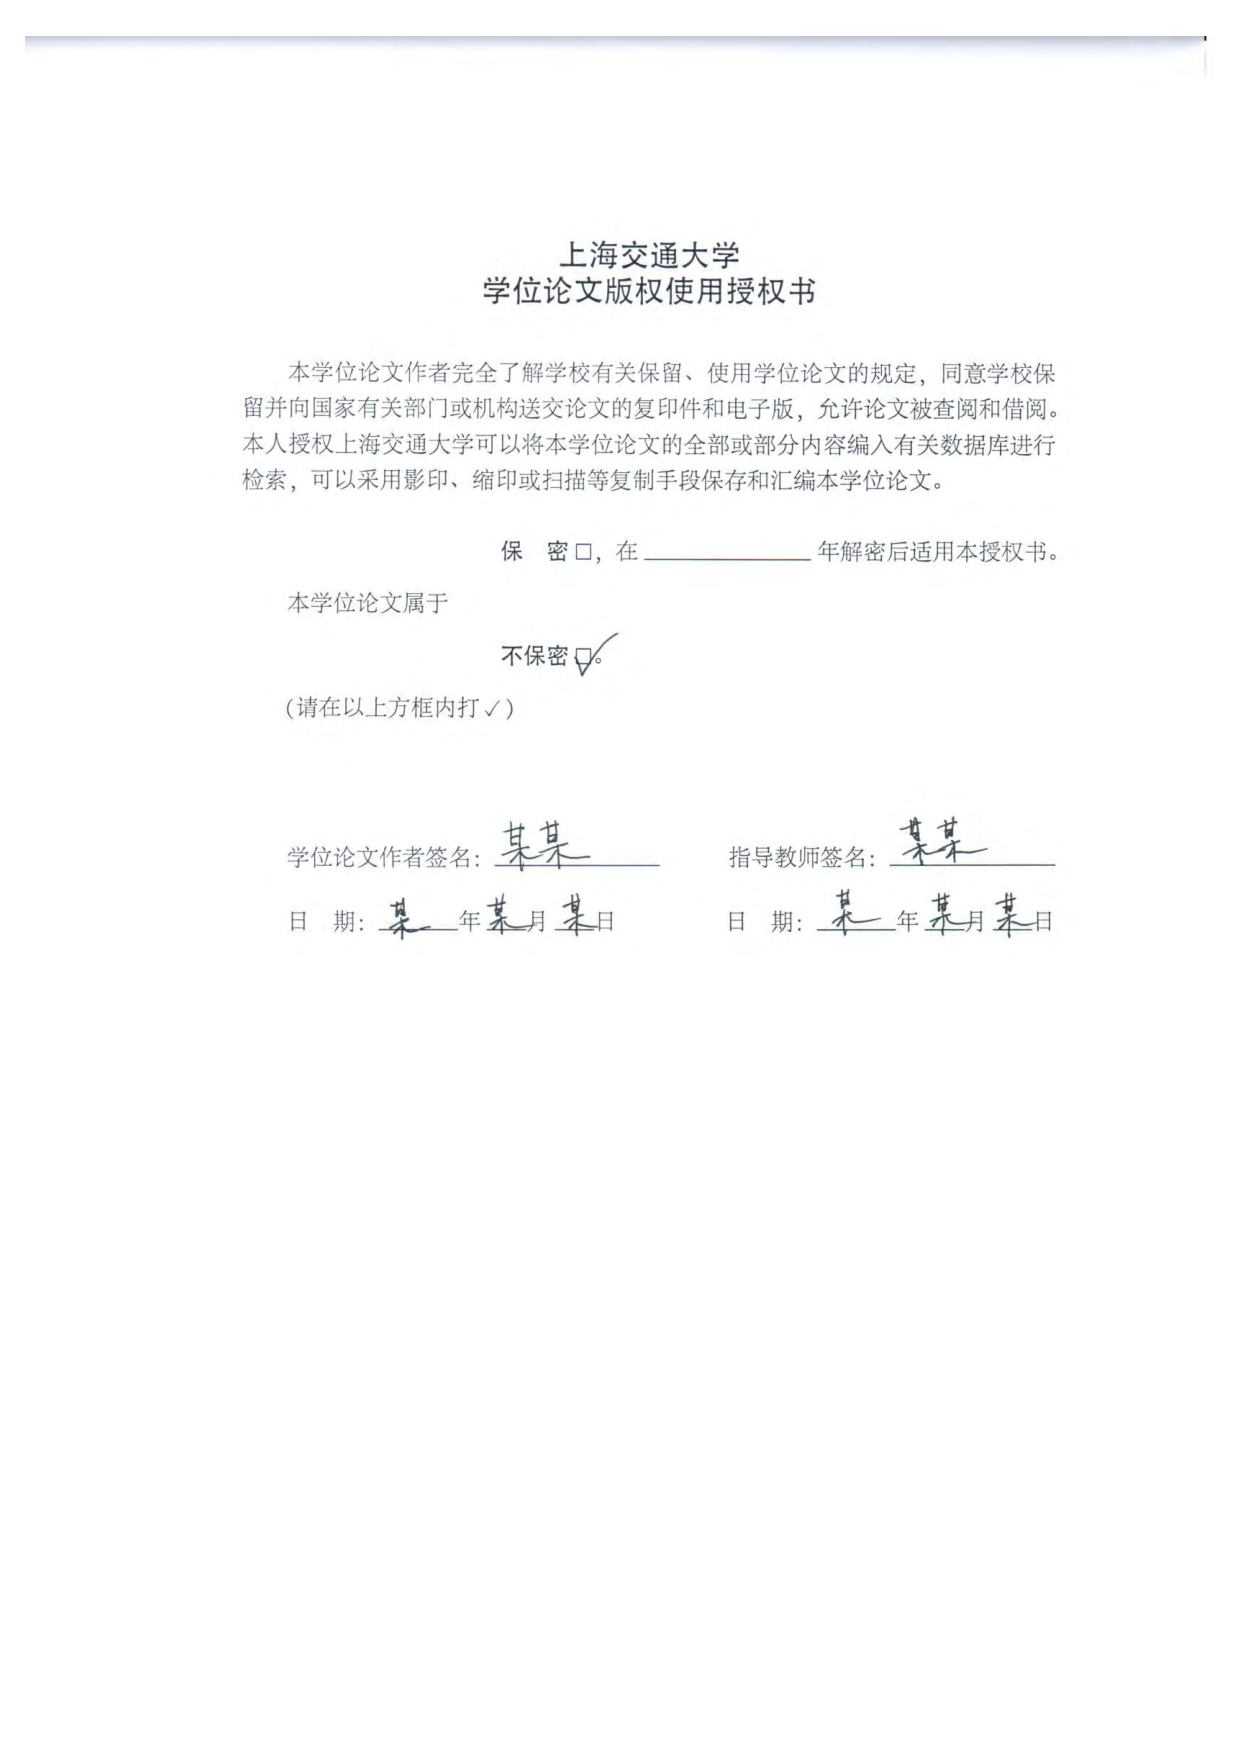
\includepdf{scans/authorization.pdf}
  \pdfbookmark[0]{\sjtu@label@authorization}{authorization}
  \cleardoublepage
\else
  \makeDeclareOriginality
  \makeDeclareAuthorization
\fi
\makeatother

%---------------------------------------------------------------------
\frontmatter

%%
%% Copyright (c) 2018 Weitian LI <liweitianux@sjtu.edu.cn>
%% Creative Commons BY 4.0
%%

% 中文摘要,约 3000 字
\begin{abstract}
\acl*{rh}如何影响 EoR 探测...
\end{abstract}

%---------------------------------------------------------------------

\begin{englishabstract}
\acs*{rh} can impose serious contamination on the EoR detection ...
\end{englishabstract}


\tableofcontents
\listoffigures
\addcontentsline{toc}{chapter}{\listfigurename}
\listoftables
\addcontentsline{toc}{chapter}{\listtablename}

\acsetup{list-style=longtable}
\printacronyms[
  include-classes=symbol,
  name={主要符号对照表},
]

%---------------------------------------------------------------------
\mainmatter
\pagestyle{main}

%%
%% Copyright (c) 2018-2019 Weitian LI <liweitianux@sjtu.edu.cn>
%% Creative Commons BY 4.0
%%

\chapter{绪论}
\label{chap:introduction}

%=====================================================================
\section{研究背景}
\label{sec:background}

理解宇宙的结构、起源和演化,是人类孜孜不倦地追求的目标,在哲学和科学中占据重要地位.
经过无数人的努力,宇宙学的\ac{bbt}终于得以建立.
该理论已被大量观测证据所支持,比如星系的红移--距离关系(即 Hubble 定律)、
\ac{cmb}辐射、星系的大尺度分布、早期元素丰度、等等,
是目前宇宙学的标准模型.

根据大爆炸宇宙学模型,宇宙起源于约 138 亿年前的一次大爆炸,然后随着宇宙的膨胀,
温度以及能量密度都逐渐降低,宇宙主要经历了\ac{inflation}、\ac{bbn}、
\ac{recomb}、\ac{da}、形成第一代天体、\ac{reion}、形成星系及大尺度结构
等阶段,如\autoref{fig:univ-history} 所示.

\begin{figure}[!htp]
  \centering
  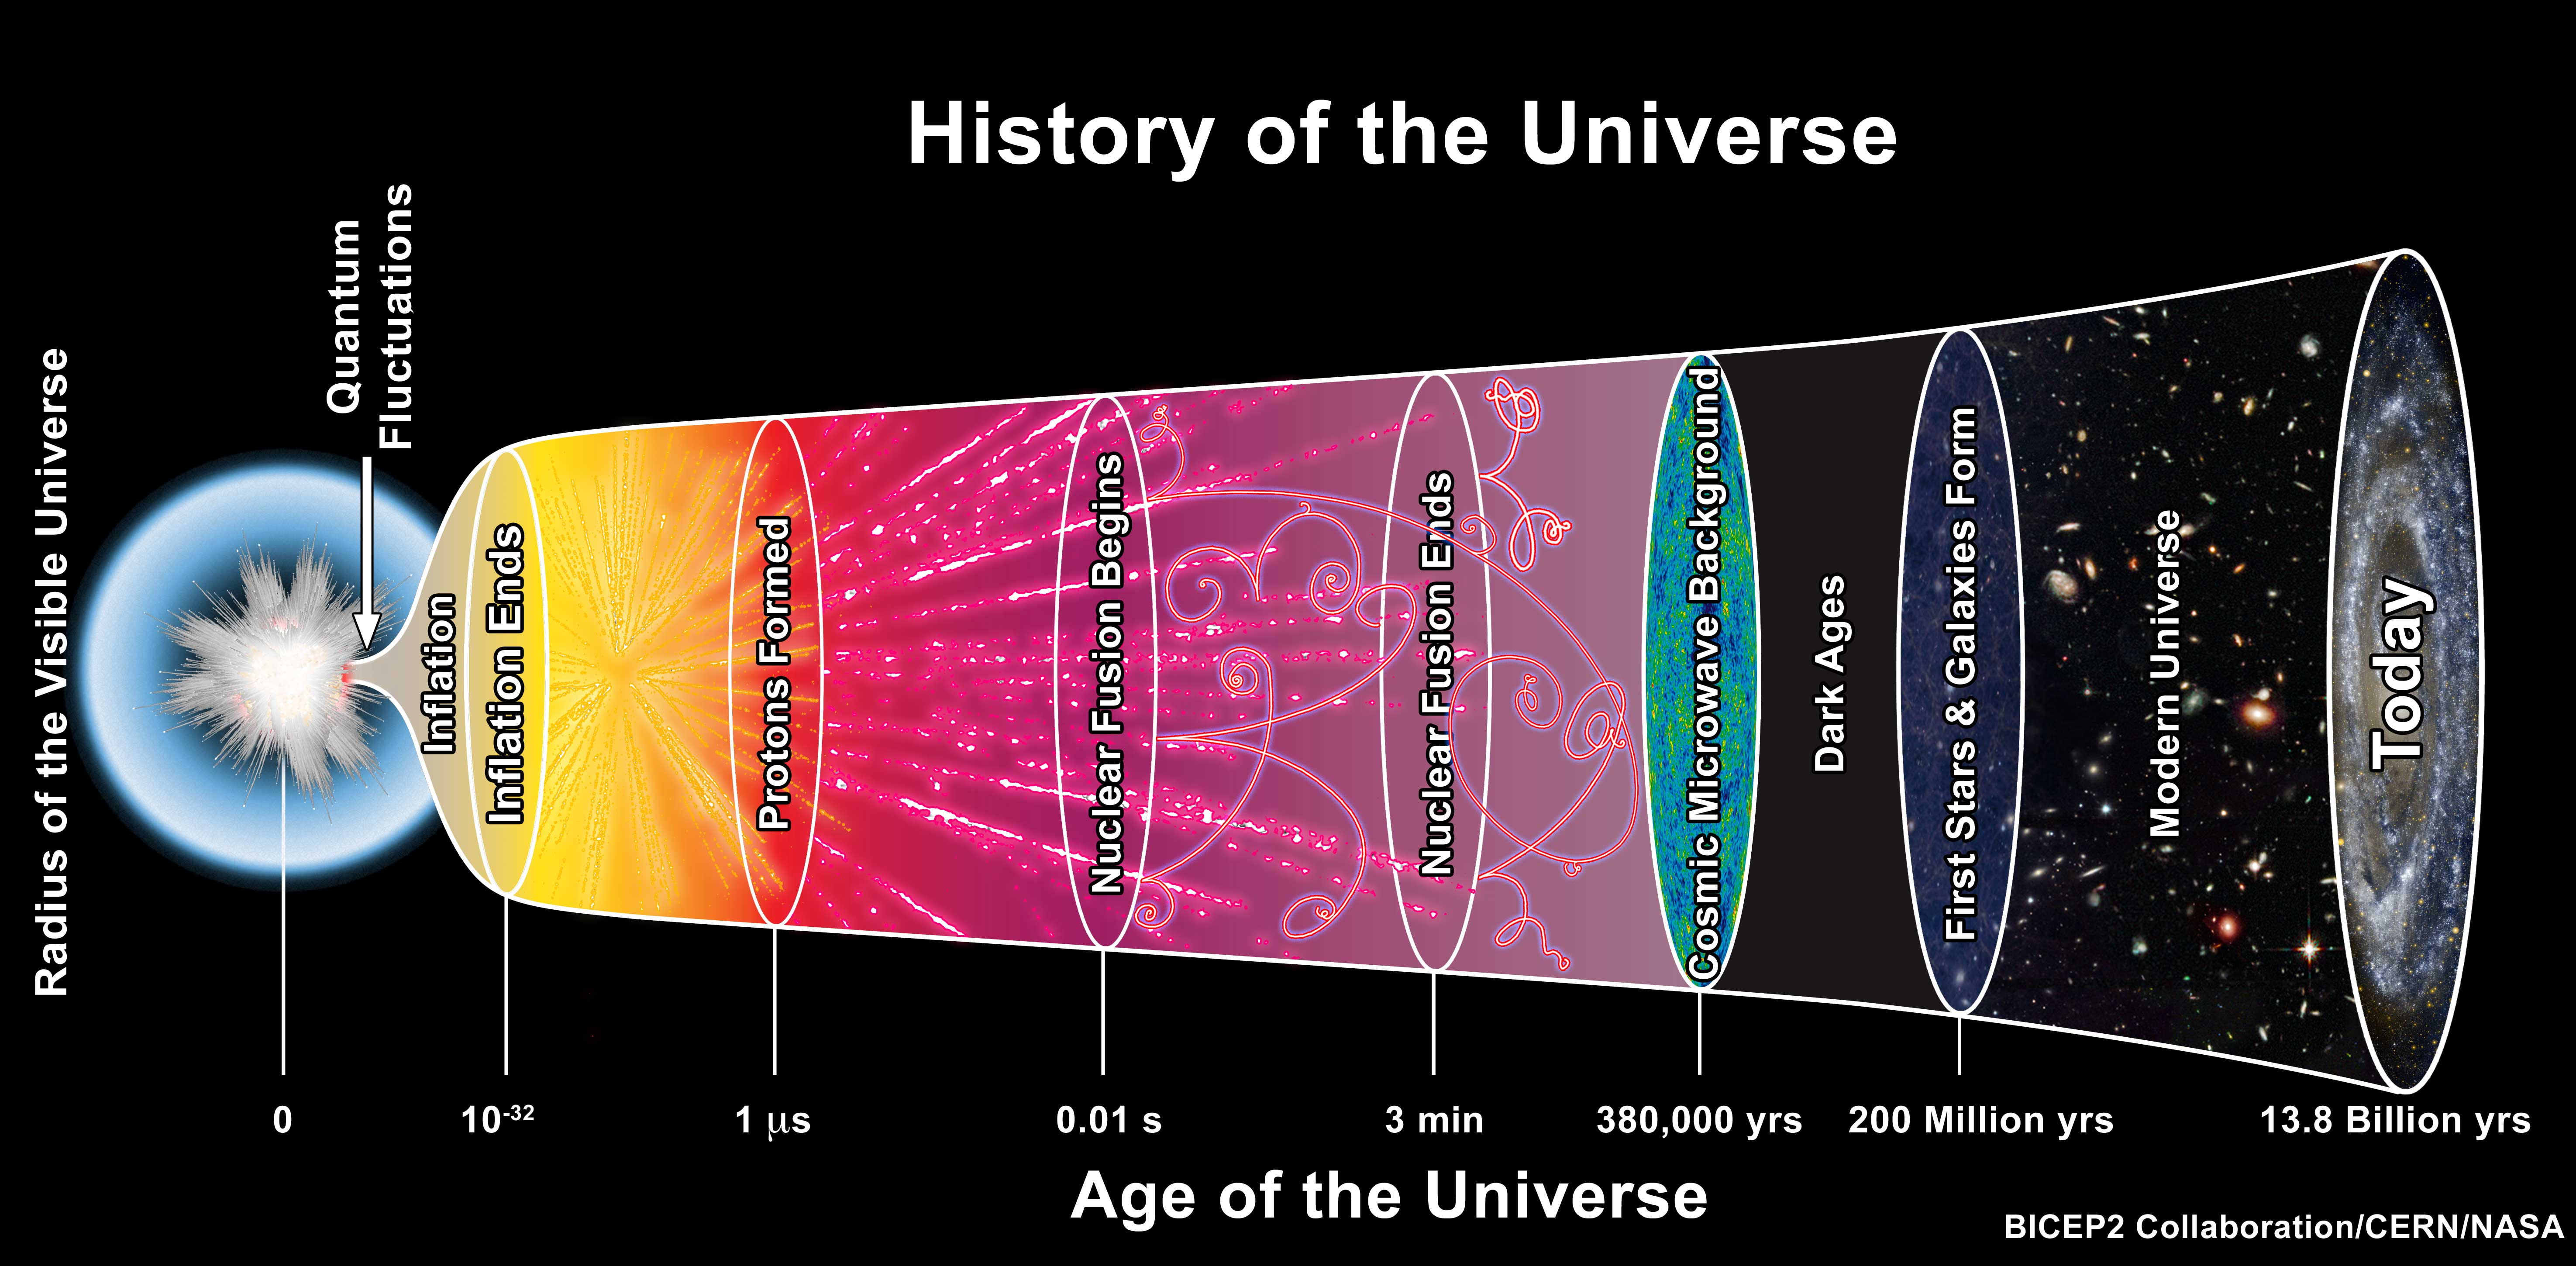
\includegraphics[width=\textwidth]{universe-history}
  \bicaption[宇宙的演化历史]{%
    宇宙从大爆炸到今天的演化历史.
  }{%
    The evolution of the Universe from the Big Bang
    to the present.
    \\\textcopyright{}
    \acuse{bicep,cern,nasa}
    \acs{bicep}2/\acs{cern}/\acs{nasa}; CC0 1.0.
  }
  \label{fig:univ-history}
\end{figure}

大爆炸之后约 40 万年,宇宙已冷却至大约 \SI{3000}{\kelvin},
于是自由电子被结合到中性原子之中,与重子物质脱耦的光子开始在宇宙中自由传播,
形成弥漫于整个宇宙的背景辐射,即今天所探测到的 \ac{cmb} 辐射.
但是,此时尚未形成发光的天体,因此宇宙进入了\acl{da}.
随着物质的密度扰动在引力作用下增长,第一代天体开始形成并产生辐射,使得重子物质
再次被逐步电离,宇宙从此结束\acl{da}并走入\ac{eor}.
随着各尺度上的天体结构的逐步形成与演化,重子物质被充分电离,宇宙也演化形成今天的格局.

\begin{figure}[!htp]
  \centering
  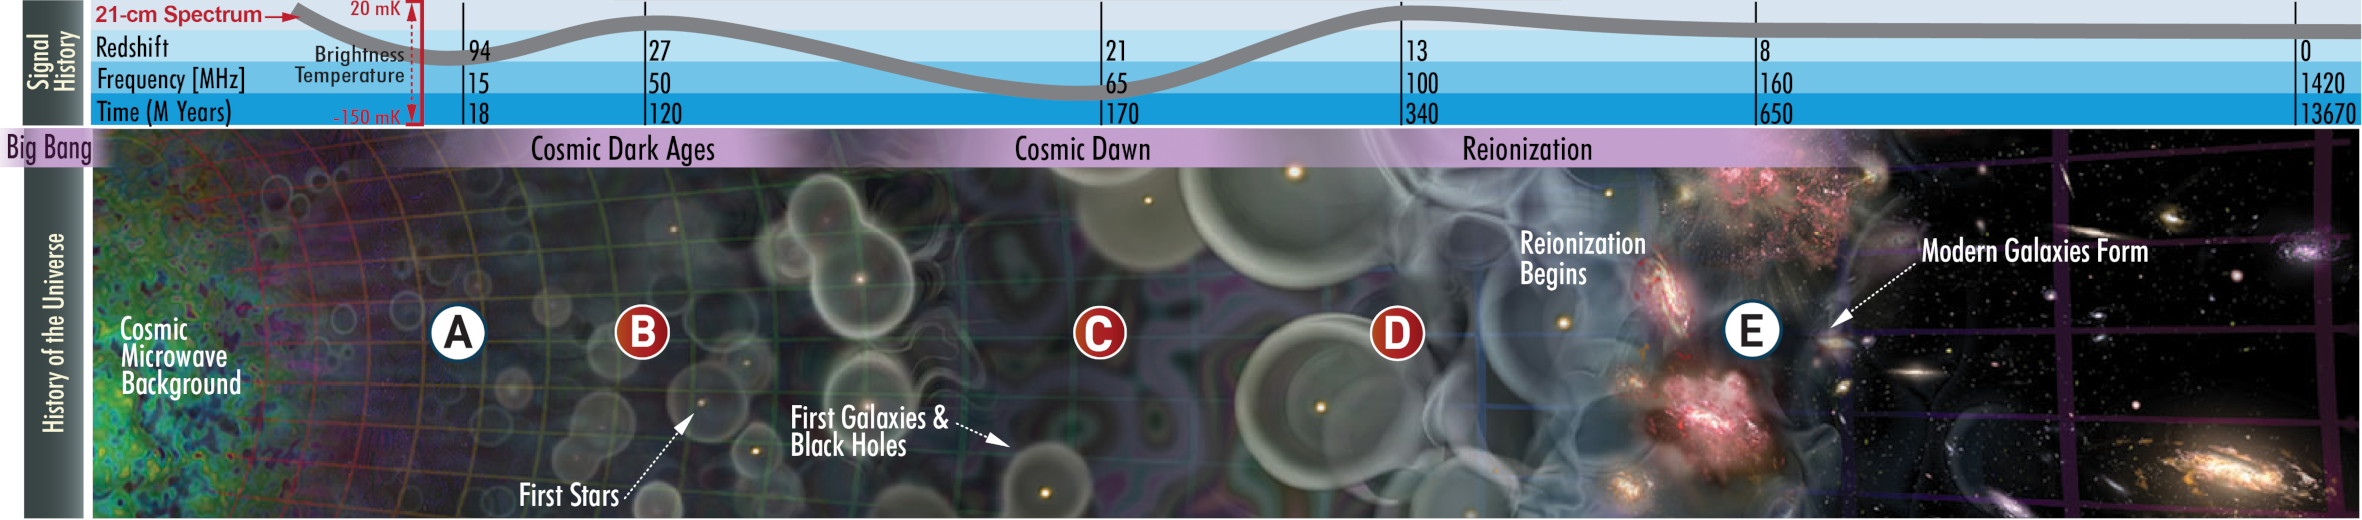
\includegraphics[width=\textwidth]{cosmic-stages-dare}
  \bicaption[宇宙的黑暗时期与再电离时期示意图]{%
    宇宙的\acl{da}与\acl{eor}示意图,其中显示了\acl{aoi} (A)、\acl{da} (B)、
    \acl{cd} (C) 以及\acl{eor} (D, E).
    上方的粗曲线显示了理论预测的 \hisignal/的强度.
  }{%
    A schematic showing the \acs{da} and the \acs{eor}
    of the Universe, mainly including the \acs{aoi} (A),
    the \acs{da} (B), the \acs{cd} (C), and the \acs{eor} (D, E).
    The thick curve in the top panel shows the predicted intensity
    of the 21\,cm signal.
    \\\textcopyright{}
    \acuse{dare}\ac{dare},
    \url{http://lunar.colorado.edu/dare/science.html}, (2018-09-23).
  }
  \label{fig:cosmic-stages}
\end{figure}

我们已借助多波段观测掌握了大量有关宇宙近期演化
($\acs{z} \lesssim 6$;宇宙已充分电离之后)的信息;
通过研究 \ac{cmb},我们对宇宙的早期历史
($z \gtrsim 1100$;自由电子\acl{recomb}之前)有了深刻理解.
然而,我们对中间的那段时期($z \sim \numrange{6}{1100}$)却知之甚少.
这段时期可细分为以下四个阶段\cite{koopmans2015}:
\acl{aoi} (\acs{aoi}; $z \sim \numrange{200}{1100}$)、
\acl{da} ($z \sim \numrange{30}{200}$)、
\acl{cd} (\acs{cd}; $z \sim \numrange{15}{30}$)
以及\acl{eor} ($z \sim \numrange{6}{15}$),
如\autoref{fig:cosmic-stages} 所示.
对于其中距离我们相对较近的\acl{eor},
我们目前仅获得非常有限的间接观测信息,比如:
该时期的\ac{hi}对高红移类星体的 Ly$\alpha$ 吸收 \cite{becker2001}、
该时期的自由电子对 \ac{cmb} 光子的 Thomson 散射 \cite{kaplinghat2003}.
但是,我们仍然缺乏来自\acl{eor}的直接观测证据,
对该时期的基本性质和关键物理过程仍不清楚,比如:
第一代天体是何时以及如何形成的?
主要的电离源有哪些以及它们是如何影响再电离过程的?
电离氢区的尺度以及演化过程如何?
研究\acl{eor}的对于理解宇宙早期结构形成以及星系的形成与演化有重要意义,
是建立完整的宇宙演化图景的关键环节之一.
具体请参见 \citeay{fan2006}, \citeay{morales2010},
\citeay{pritchard2012}, \citeay{zaroubi2013},
\citeay{koopmans2015} 等综述文.

在\acl{eor}及其之前的\acl{da},尽管缺乏发光天体可供观测,
但是宇宙中丰富的\acl{hi}所辐射的 21\,cm 谱线
(以下简称 \emph{\hisignal/};
详见 \autoref{sec:21cm-signal})为探测该时期提供了有效途径.
对 \hisignal/的探测是目前对\acl{eor}及其之前的\acl{da}开展系统性
研究的最直接而有效的观测手段 \cite{koopmans2015,furlanetto2016}.

\acl{hi}的 21\,cm 谱线的本征频率约为 \SI{1420}{\MHz}.
源自\acl{eor}的 \hisignal/(以下简称 \emph{EoR 信号})经历显著红移后
应出现在约 \SIrange{90}{200}{\MHz},对应低频射电波段.
EoR 信号到达地球时已非常微弱,仅约几 \si{\mK} 至十几 \si{\mK},
因此需要具有极高灵敏度的低频观测设备才能捕获该信号.
目前的主流技术是采用大规模低频干涉阵列,已建成或正在建设的干涉阵列主要有:
\ac{21cma} \cite{zheng2016}、
\ac{gmrt} \cite{paciga2011}、
\ac{mwa} \cite{bowman2013,tingay2013}、
\ac{lofar} \cite{vanHaarlem2013}、
\ac{lwa} \cite{ellingson2009}、
\ac{paper} \cite{parsons2010}、
\ac{hera} \cite{deboer2017}、
\ac{ska} \cite{mellema2013,koopmans2015}.
然而,利用干涉阵列探测 EoR 信号仍面临诸多困难与挑战,其中主要包括:
识别并扣除强烈的前景干扰、扣除人工源的\ac{rfi}、修正电离层的扰动、
苛刻的仪器校准要求、海量数据处理和高动态范围成像.

在低频射电波段,强烈的前景干扰(主要源自银河系以及河外点源;
详见 \autoref{sec:fg-intro})比待探测的 EoR 信号高出约 5 个数量级;
即便按干涉阵列所测量的天空亮度涨落来衡量,前景干扰的涨落也是待测信号的数千倍
\cite{zaroubi2013}.
如何准确把握前景干扰并将其有效扣除,是成功探测 EoR 信号的关键.
由于低频射电观测和巡天数据的严重不足,我们对该波段的前景的了解非常有限,
无法达到探测 EoR 信号所要求的精度.
因此,我们需要挖掘已有海量的中高频射电观测以及其他多波段观测数据,
并结合逐渐增长的低频观测数据,深入理解低频射电前景辐射,构建并完善前景模型,
为识别并扣除前景干扰提供有力支撑.

虽然在本质上,前景辐射的频谱是光滑的,而 EoR 信号的频谱呈锯齿状,
两者具有很好的可区分性 \cite{wang2006,jelic2008,harker2009,wang2013}.
然而在实际情况中,受到干涉阵列的复杂仪器效应、观测干扰、数据处理技术的限制
等因素的影响,前景频谱的光滑性遭到破坏,导致 EoR 信号的提取变得尤其困难
\cite{liu2009ps,labropoulos2009,gehlot2018,mertens2018}.
如何研发出行之有效的前景处理和 EoR 信号提取算法,亦是当前的重要研究课题.


%=====================================================================
\section{研究内容}
\label{sec:content}

本文的研究内容分为以下两部分:
\begin{itemize}
\item
\emph{改进低频射电天空的模拟:}
深刻理解各前景成分的性质(如强度、空间分布、频谱结构)并充分把握它们对 EoR 探测
的干扰方式,是研发具有针对性的前景去除和 EoR 信号分离算法的前提与关键 (ref???).
由于复杂的仪器效应和严重的观测干扰,低频干涉阵列的系统校准非常困难
\cite{noordam2004,intema2009,wijnholds2010,barry2016,gehlot2018},
严重制约仪器达到探测 EoR 信号所要求的极高灵敏度.
在现阶段缺乏足够可用的高质量低频射电观测数据的情况下,挖掘已有多波段观测数据并
准确模拟低频射电天空,是开展前景干扰研究以及 EoR 信号分离算法研发的可行办法.

\hspace{2\ccwd}%
在诸多前景成分之中,银河系的弥散辐射 [包括\ac{synrad}和\ac{brad}]
以及河外\ac{pntsrc}辐射是最主要的成分,目前已被广泛地研究和较好地理解
\cite{shaver1999,diMatteo2004,gleser2008,liu2012,murray2017,spinelli2018}.
除此之外,剩下的前景辐射主要来自河外\ac{extsrc},其中包括:
\ac{icm} \cite{feretti2012} 产生的\ac{rh}、\ac{rr}和\ac{rmh}、
\ac{gc}之外的\ac{igm} \cite{keshet2004}、
以及\ac{lsf} \cite{vazza2015}.
对于这些河外\acl{extsrc},已获得的观测证据不多,在低频射电波段更是不足.
关于它们将具体如何影响 EoR 探测,目前的理解非常有限,亟待深入且系统的研究.

\hspace{2\ccwd}%
与其他几类河外\acl{extsrc}相比,\acl{rh}拥有更多的观测证据和理论研究,支撑我们
构建一个更佳的模型用来模拟\acl{rh}的低频射电辐射,改进低频射电天空的模拟,
进而在考虑干涉阵列的实际仪器效应的情况下,有效地评估\acl{rh}对 EoR 探测的影响.

\item
\emph{研发 EoR 信号分离新算法:}
为了提取淹没于前景干扰中的 EoR 信号,一系列方法已被提出来用于处理前景
(详见 \autoref{sec:fg-methods}).
这些前景处理方法可大致分为\ac{fgrm}和\ac{fgavd}两大类,
但都依赖于一个重要前提:前景辐射的频谱必须非常光滑.
据此,这些方法通过构建一个模型来拟合光滑的前景成分并扣除,或者在功率谱空间尽量
避开前景污染区域,从而提取出微弱的 EoR 信号 \cite{chapman2016}.

\hspace{2\ccwd}%
然而在实际情况中,干涉阵列的\ac{beam}存在频率依赖效应(以下简称\emph{波束效应}),
即\acl{beam}的形状随观测频率而变化,因此 CLEAN 后残留的前景源会产生沿频率方向
快速变化的涨落,严重破坏前景频谱的光滑性 \cite{liu2009ps},
导致现有方法无法有效分辨前景干扰与 EoR 信号并分离出 EoR 信号
(详见 \autoref{sec:fdeffect}).

\hspace{2\ccwd}%
考虑到干涉列阵的\acl{beam}的形状非常复杂,为现有方法打造一个实际可用的模型
用以克服上述复杂的波束效应将很困难 \cite{lochner2015},
因此研发基于\ac{dl}的 EoR 信号分离新算法是一条更加可行且具有吸引力的途径
\cite{herbel2018,vafaeiSadr2019},
通过从数据中学习知识并自适应地优化模型,达到克服波束效应并分离 EoR 信号的目标.

\end{itemize}

本文的研究目标是:
(1)改进\acl{rh}的模拟,考虑干涉阵列的实际仪器效应,
获得更精细、更符合实际的低频射电天空的模拟图像,
进而有效地评估\acl{rh}对 EoR 探测的影响.
(2)研发基于\acl{dl}的能够有效克服干涉阵列的波束效应的 EoR 信号分离新算法,
并运用到上述模拟数据进行测试和优化.


%=====================================================================
\section{研究方案}
\label{sec:plan}

本文遵循以下主要步骤开展开展工作,完成研究内容,达到研究目标:
\begin{enumerate}
\item
调研\acl{rh}的相关理论研究和观测证据,理解其形成机制和演化规律,
构建模型并编程实现模拟\acl{rh}的低频射电辐射.
搜集\acl{rh}的现有观测数据,调节模型的参数,获得可靠的模拟结果.

\item
采用典型的干涉阵列(如 SKA1-Low)的布局方案,对上一步所得的\ac{skymap}
开展模拟观测,得到\ac{vis}数据,再利用 CLEAN 算法成像获得相应的“观测”图像.
通过这种\ac{e2e}模拟,干涉阵列的复杂仪器效应(如本文关注的波束效应)得以
有效地整合到研究流程之中.

\item
基于上述模拟所得的“观测”图像,利用一维和二维\ac{ps},对比\acl{rh}和
EoR 信号的异同,量化\acl{rh}在运用\acl{fgrm}或\acl{fgavd}的情况下
对 EoR 探测的影响,有效评估\acl{rh}作为前景干扰成分的重要程度.

\item
对比分析目前的主流\acl{dl}方法,筛选出合适的算法并加以必要的改进,
适用到此处的 EoR 信号分离场景.
利用已有模拟数据对算法进行训练和调优,挑选出满足要求的最佳算法.

\end{enumerate}


%=====================================================================
\section{本文框架}
\label{sec:structure}

本文余下章节安排如下:
\autoref{chap:interferometry}将介绍射电天文学和射电干涉技术的基础知识,
包括基本辐射理论、天线原理、干涉阵列及综合孔径成像等.
在\autoref{chap:detection},我们将介绍利用\acl{hi}
\hisignal/探测宇宙再电离时期的方法和困难、以及前景处理方法.
在\autoref{chap:simulation},我们首先模拟各前景成分和 EoR 信号的\acl{skymap},
然后进行干涉阵列的模拟观测,得到整合了实际仪器效应的观测图像.
据此,我们在\autoref{chap:halo}借助\acl{ps}量化评估\acl{rh}对
EoR 探测的具体影响.
\autoref{chap:cdae}将阐述我们提出的基于\acl{dl}的 EoR 分离新算法并演示其效果.
最后,我们对全文进行总结并简要展望.

全文采用一个由 \lcdm/ 模型描述的平直宇宙,具体参数为:
$\acs{H0} = 100\,\acs{h} = \SI{71}{\km\per\second\per\Mpc}$、
$\acs{Om0} = 0.27$、
$\acs{Ol0} = 1 - \acs{Om0} = 0.73$、
$\acs{Ob0} = 0.046$、
$\acs{ns} = 0.96$ 以及 $\acs{sigma8} = 0.81$.
如无额外说明,本文给出的误差对应 \SI{68}{\percent} 的置信水平;
使用的幂律谱形式为 $\acs{Sfreq} \propto \acs{freq}^{-\acs{Sidx}}$,
其中 \acs{Sfreq} 为\acl{Sfreq}、\acs{Sidx} 为\acl{Sidx}.
本文使用的中文术语遵循《英汉天文学名词数据库》
\footnote{英汉天文学名词数据库:\url{http://astrodict.china-vo.org/}}.


%% EOF

%%
%% Copyright (c) 2018-2019 Weitian LI <liweitianux@sjtu.edu.cn>
%% Creative Commons BY 4.0
%%

\chapter{射电天文学基础}
\label{chap:radio-astronomy}

%=====================================================================
\section{射电天文学简介}

%---------------------------------------------------------------------
\subsection{简介和历史}

我们对宇宙的几乎所有认识都来自于观测并研究所接收到的电磁辐射,
在射电波段对天体和宇宙开展研究的天文学分支称为\emph{射电天文学 (radio astronomy)}.
对于地面上的射电望远镜,观测频率的下限约为 $\nu_{\R{min}} \sim \SI{10}{\MHz}$
($\lambda_{\R{max}} \sim \SI{30}{\meter}$),
取决于\ac{ionosphere}的截断频率,低于该频率的电磁波将被反射而无法到达地面.
观测频率的上限约为 $\nu_{\R{max}} \sim \SI{1000}{\GHz}$
($\lambda_{\R{min}} \sim \SI{0.3}{\mm}$),主要原因是\ac{troposphere}中的
分子(主要是 $\mathrm{H_2 O}$ 和 $\mathrm{O_2}$)的最低转动能带的共振吸收.
\autoref{fig:atmospheric-emt} 显示了大气层的电磁辐射透射率以及相应的射电观测窗口.

\begin{figure}[htp]
  \centering
  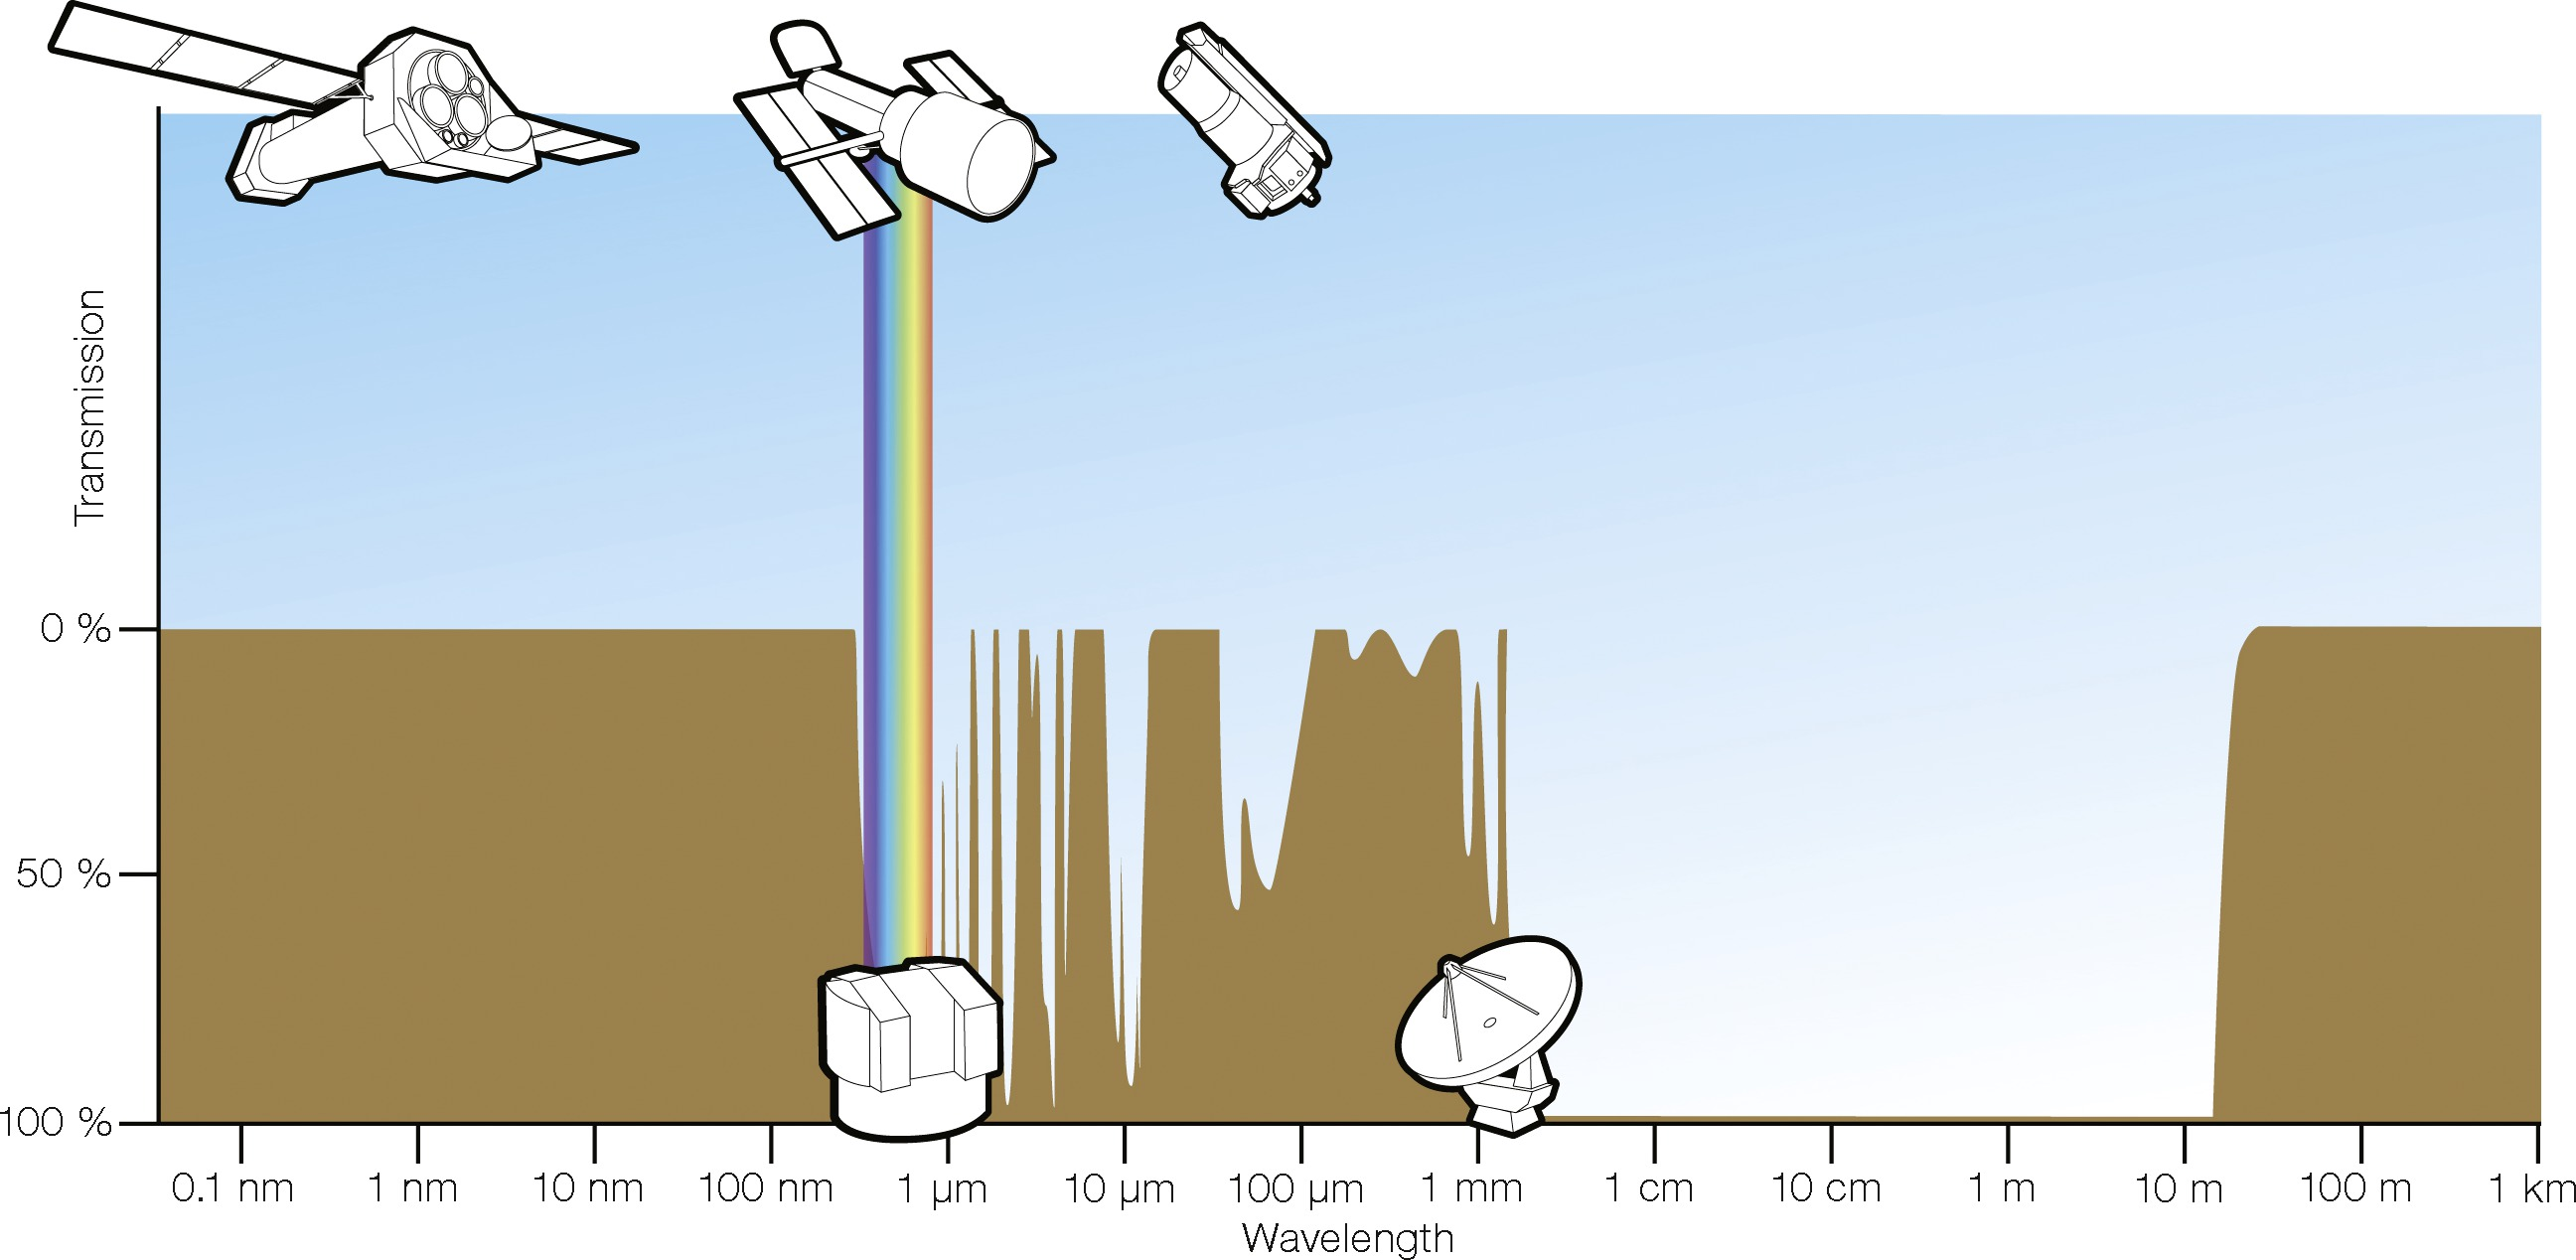
\includegraphics[width=\textwidth]{atmospheric-em-transmittance}
  \bicaption[大气层的电磁辐射透射率]{%
    大气层的电磁辐射透射率随波长(即频率)的变化.
    除了光学窗口,大气层还有一个更加宽广的射电窗口,
    从 $\lambda \sim \SI{0.3}{\mm}$ ($\nu \sim \SI{1000}{\GHz}$)
    延伸到 $\lambda \sim \SI{30}{\meter}$ ($\nu \sim \SI{10}{\MHz}$).
    大气层对电磁辐射的吸收情况会随时间以及地理位置而变化.
  }{%
    Electromagnetic transmittance of the Earth's atmosphere.
    In addition to the visible optical window, there is another
    much wider radio window, which spans from
    $\lambda \sim \SI{0.3}{\mm}$ ($\nu \sim \SI{1000}{\GHz}$)
    to $\lambda \sim \SI{30}{\meter}$ ($\nu \sim \SI{10}{\MHz}$).
    \\\textcopyright{}
    \citeay{condon2016}, \S\,1.1.2.
  }
  \label{fig:atmospheric-emt}
\end{figure}

首次发现源自地球之外的射电辐射是在 1932 年被 Bell 电话实验室的工程师
Karl Guthe Jansky 意外得到的.
上世纪 20 年代,Bell 电话公司基于短波($\lambda \sim \SI{15}{\meter}$)传输
建设了跨洋电话服务,但是发现通话受到了强烈的干扰,因此 Bell 电话实验室派
Jansky 去查明干扰来源.
Jansky 建造了一个对方向敏感的可转动天线(如\autoref{fig:jansky-antenna} 所示)
用来监测 \SI{20.5}{\MHz} ($\lambda \approx \SI{14.6}{\meter}$) 处的射电辐射.
经过观测,他发现绝大部分的干扰源自暴风雨的闪电.
此外,他还发现有一个较弱的不明噪声,其强度在每天发生周期性的变化,
他怀疑该噪声可能源自太阳的射电辐射.
但是持续的观测显示该不明噪声的准确周期为 \SI{23}{\hour}\,\SI{56}{\minute},
并不是刚好 \SI{24}{\hour}.
将此困惑与他的一个天文学家朋友 Albert Melvin Skellett 讨论后,
Jansky 了解到该噪声应来自太阳系之外,并进一步确认其来源是银河系中心 \cite{jansky1933}.

\begin{figure}[htp]
  \centering
  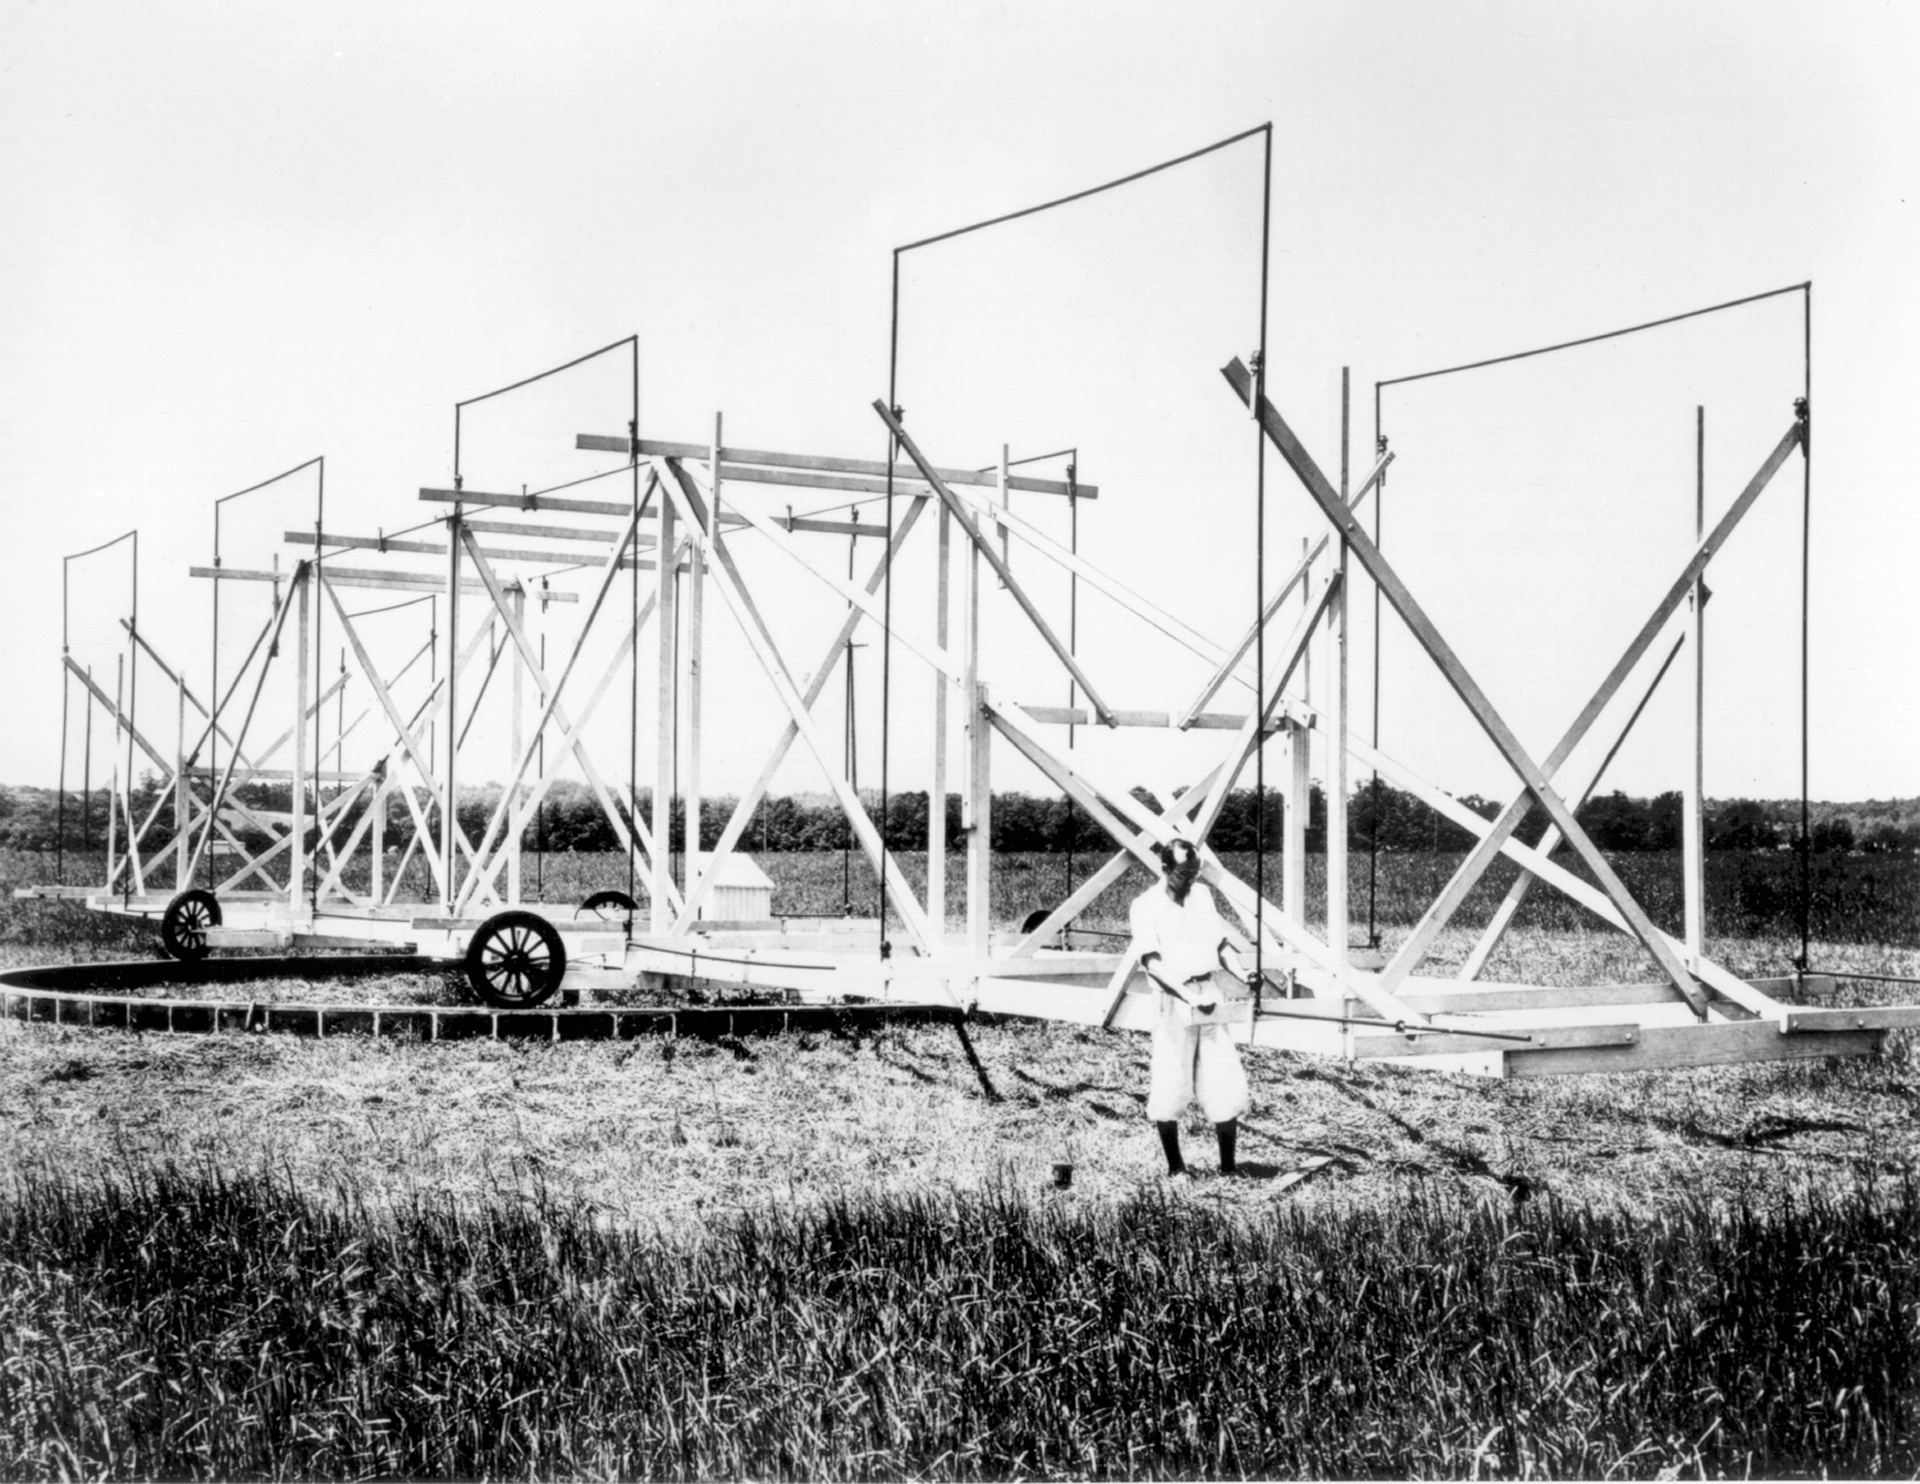
\includegraphics[width=0.8\textwidth]{KarlJansky-antenna}
  \bicaption[Karl G. Jansky 和他的天线]{%
    Karl G. Jansky 和他的天线.
    该天线可转动,主要接收水平方向的辐射.
  }{%
    Karl G. Jansky and the antenna that discovered the cosmic radio emission.
    The antenna can rotate in azimuth and mainly receive horizontal
    emissions.
    \\\textcopyright{}
    \acuse{nrao,aui,nsf}\acs{nrao}/\acs{aui}/\acs{nsf}.
  }
  \label{fig:jansky-antenna}
\end{figure}

然而,Jansky 的发现未能得到足够的关注和重视,他本人也被分配到其他项目而无法继续
详细研究银河系的射电辐射.
幸运的是,另一位无线电工程师 Grote Reber 对 Jansky 的发现产生了极大兴趣,
于是耗费数年在自家后院建造了世界第一台抛物面射电望远镜
(如\autoref{fig:reber-telescope} 所示).
在 1938 年,Reber 用这台望远镜成功地在 \SI{160}{\MHz} 探测到了银河系的辐射.
他进一步开展了银河系的第一次射电巡天观测,这些结果发表于专业的天文期刊
\apj \cite{reber1940},使得 Jansky 的成果得到了应有的重视.

\begin{figure}[htp]
  \centering
  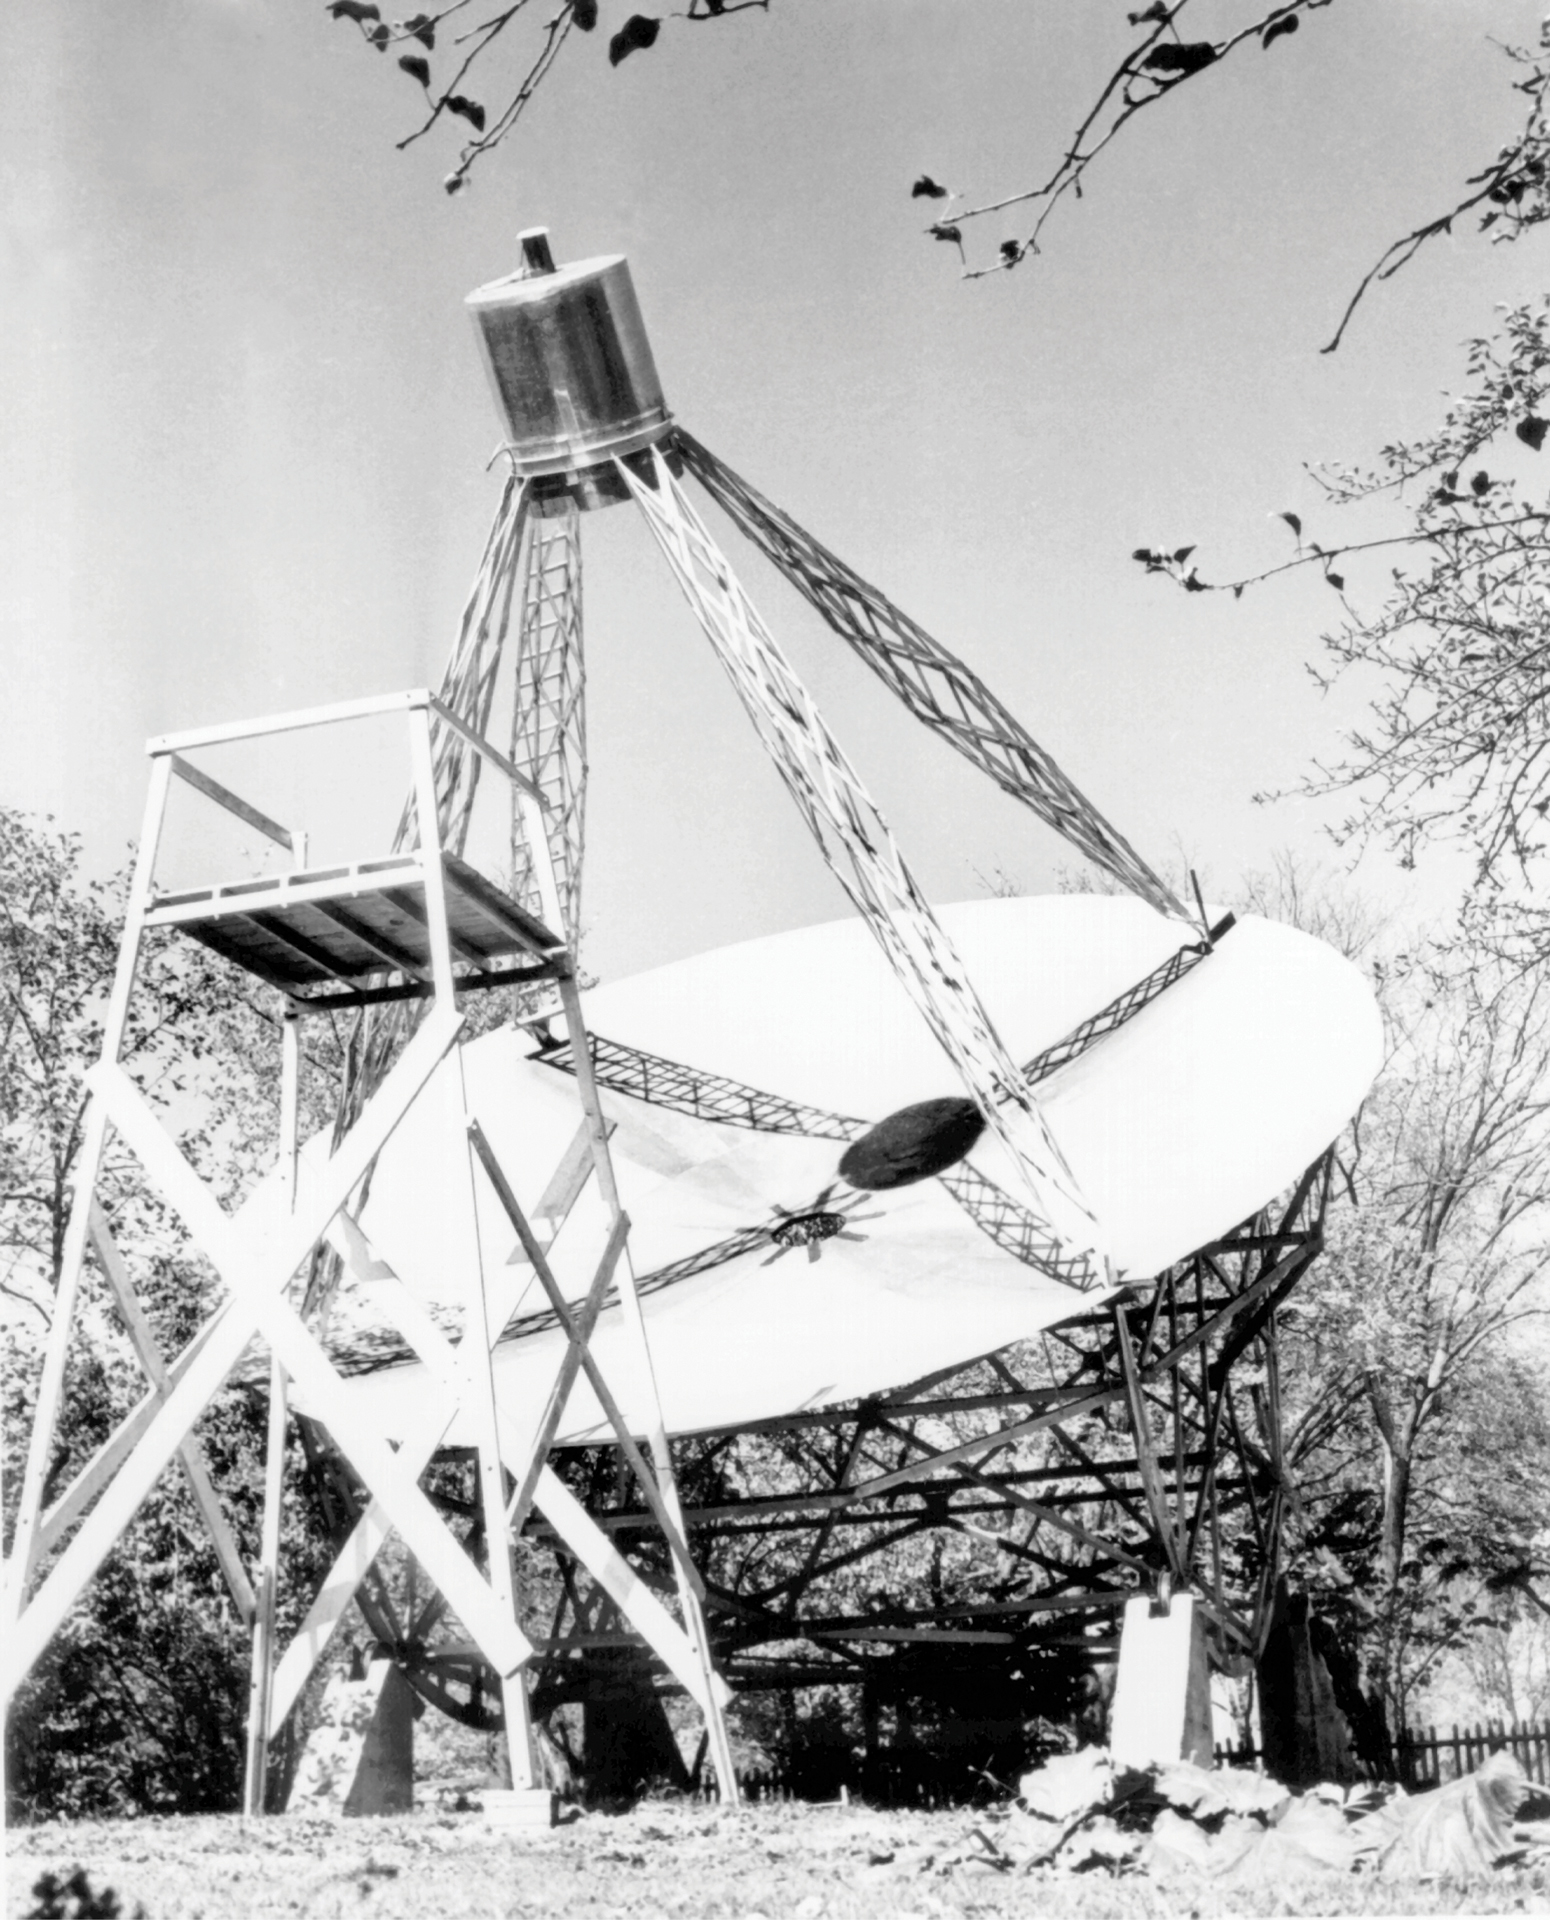
\includegraphics[width=0.6\textwidth]{GroteReber-telescope}
  \bicaption[Grote Reber 的射电望远镜]{%
    Grote Reber 在自家后院建造的射电望远镜,使用了直径约 \SI{10}{\meter} 的抛物面.
  }{%
    Grote Reber's backyard radio telescope using a parabolic reflector
    of diameter about \SI{10}{\meter}.
    \\\textcopyright{}
    \acs{nrao}/\acs{aui}/\acs{nsf}.
  }
  \label{fig:reber-telescope}
\end{figure}

后续的几年里,尽管第二次世界大战阻碍了射电天文的发展,但是极大地刺激了无线电技术
和雷达设备的研发.
这些方面的成果在战争结束后给射电天文学带来了长足进步,开创了一系列新技术和新方法.
其中最值得一提的是由 Martin Ryle 和 Antony Hewish 发明的\ac{as}技术,
使射电观测的角分辨率和灵敏度得到了空前的提高.

自射电窗口被打开以来,射电天文学已取得了一系列激动人心的新发现,主要包括:
银河系和其他多种天体的非热辐射 \cite{reber1940}、
由超大质量黑洞驱动的射电星系\cite{baade1954}和\ac{quasar}\cite{hazard1963,schmidt1963}及其演化、
冷星际介质(如原子、离子和分子)的热辐射谱线、
星际分子的\ac{maser} \cite{weaver1965}、
源自宇宙大爆炸的 \ac{cmb} \cite{penzias1965}、
\ac{pulsar}和中子星 \cite{hewish1968}、
星系的 \ac{hi} 旋转曲线显示其内部存在\ac{dm} \cite{roberts1975}、
强\ac{gl} \cite{walsh1979}.
总之,射电天文学揭开了宇宙在光学波段所见完全不同的一面(如\autoref{fig:radio-sky} 所示),
极大地促进了我们对宇宙的认识,深刻地改变了我们对宇宙的理解.

\begin{figure}[htp]
  \centering
  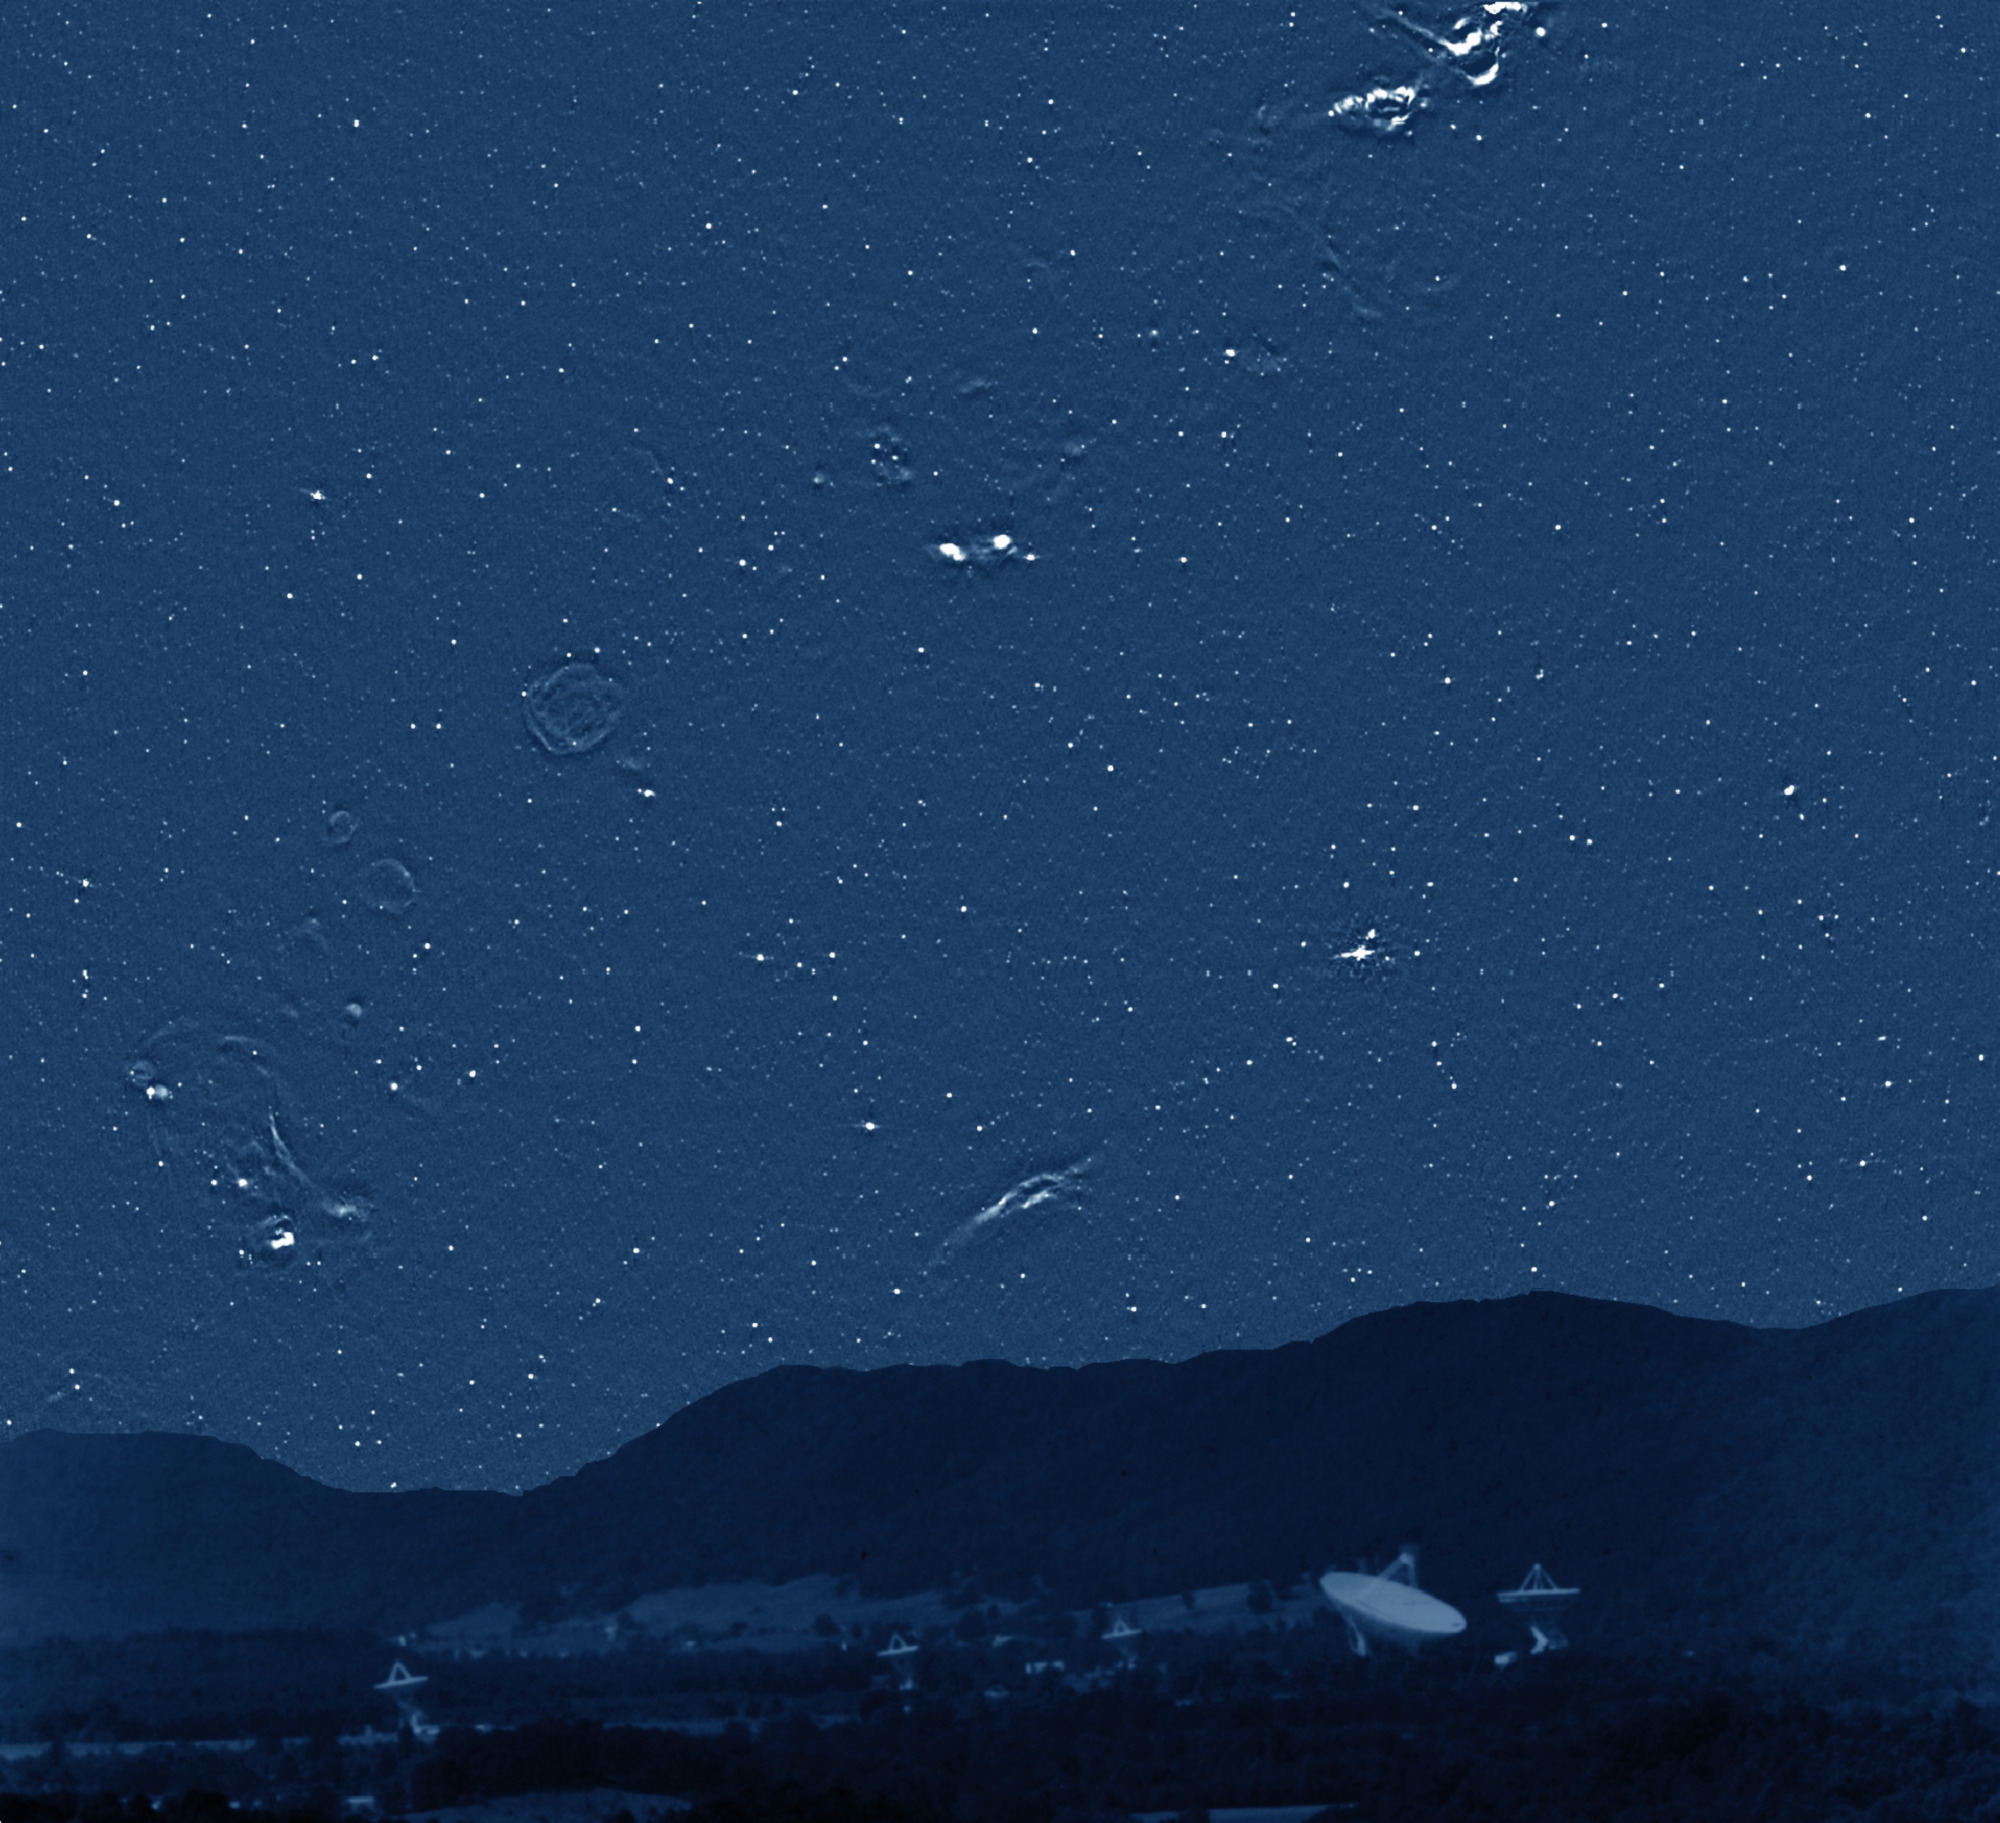
\includegraphics[width=0.8\textwidth]{nrao-radio-sky}
  \bicaption[与光学波段所见完全不同的射电天空]{%
    在 NRAO 台址的照片上方显示了由 NRAO 前 \SI{91}{\meter} 射电望远镜获得的
    \SI{4.85}{\GHz} 射电天空图像.
  }{%
    The \SI{4.85}{\GHz} radio sky made with the NRAO former \SI{91}{\meter}
    telescope is shown above an old photograph of the NRAO site.
    \\\textcopyright{}
    \acs{nrao}/\acs{aui}/\acs{nsf}.
  }
  \label{fig:radio-sky}
\end{figure}

%---------------------------------------------------------------------
\subsection{机遇和挑战}

尽管大气层的射电窗口允许低至约 \SI{10}{\MHz} 的观测,但由于各种技术和条件的限制,
以往的射电观测和研究主要位于 $\gtrsim \si{\GHz}$ 的中高频波段.
相比中高频波段,低频波段(约 \SIrange{50}{300}{\MHz})主要有以下几点优势:
\begin{itemize}
  \item 低频波段对应的辐射波长更长,受尘埃的影响更小,因此能够观测到星系更核心的区域.
  \item \ac{synrad}在低频波段更强且寿命更长,因此更利于探测\ac{gc}、
    \ac{sc}甚至\ac{lsf}的弥散射电辐射.
  \item 多种等离子体效应(如散射、色散、Faraday 旋转)的强度按 $\nu^{-2}$ 变化,
    因此在低频波段更适合研究星际电子密度、磁场强度、等等.
  \item 源自宇宙再电离时期 (红移 $z \sim \numrange{6}{16}$)
    的\ac{hi} 21\,cm 信号历经红移后将出现在低频波段,因此不可避免地需要在
    此波段开展观测,探测该信号以研究宇宙早期的再电离过程
    (详见 \autoref{sec:eor-signal}).
  \item 低频射电望远镜通常具有大视场,能够显著提高巡天速度,非常有利于搜寻
    脉冲星、暂现源、等等.
\end{itemize}

随着相关技术取得了充分发展,低频射电波段已在近十多年来得到了重点关注并取得了长足进步,
目前已建成一批工作在此波段的干涉阵列,
主要包括 \ac{21cma}、\ac{gmrt}、\ac{mwa}、\ac{lofar}.
此外还有若干正在积极建设的新型低频干涉阵列,比如 \ac{lwa}、\ac{hera}、\ac{ska}.
可见,低频射电波段正在成为射电天文及至整个天文领域的热点和前沿,

当然,在低频波段开展观测也面临更大的挑战,
比如强烈的人工源\ac{rfi}、\ac{ionosphere}的扰动、
通常需要建设更大更复杂的干涉阵列、解决更复杂的仪器效应、
研发更有效的数据处理方法(参见 \autoref{sec:det-difficulties}).
尽管如此,可以肯定低频射电天文将成为射电天文领域的重要力量,
并为整个天文学的发展作出不可磨灭的贡献.


%=====================================================================
\section{辐射基础}
\label{sec:radiation}

%---------------------------------------------------------------------
\subsection{亮度和流量密度}

\begin{figure}[htp]
  \centering
  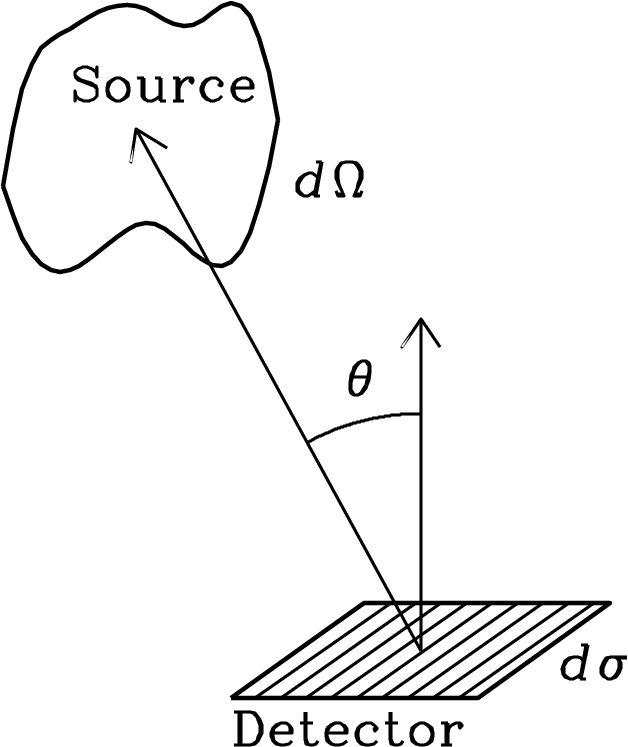
\includegraphics[width=0.3\textwidth]{specific-intensity}
  \bicaption[\acl*{I-nu} \acs*{I-nu} 的测量]{%
    \acl*{I-nu} \acs*{I-nu} 的测量示意图.
  }{%
    The specific intensity \acs*{I-nu} measured by a detector of area
    $\D{\sigma}$ to a source extending a solid angle of $\D{\Omega}$.
    \\\textcopyright{}
    \citeay{condon2016}, \S\,2.1.
  }
  \label{fig:intensity}
\end{figure}

考虑一个面积为 $\D{\sigma}$ 的探测器,测量一个与其法线方向呈 $\theta$ 角度、
所张立体角为 $\D{\Omega}$ 的源的辐射(如\autoref{fig:intensity} 所示),
若探测器在频率范围 $[\nu, \,\nu+\D{\nu}]$ 内接收到的功率为 $\D{P_{\nu}}$,
则源的\emph{\acf{I-nu}} 为:
\begin{equation}
  \label{eq:intensity}
  \acs{I-nu} \equiv
    \frac{\D{P_{\nu}}}{(\cos\theta\,\D{\sigma}) \,\D{\nu} \,\D{\Omega}} \,,
\end{equation}
其单位是 [\si{\watt\per\square\meter\per\hertz\per\steradian}].
\acl{I-nu} \acs{I-nu} 亦被称为\emph{谱亮度 (spectral brightness)},
有时也被简称为\emph{强度}或\emph{亮度}.

\begin{figure}[htp]
  \centering
  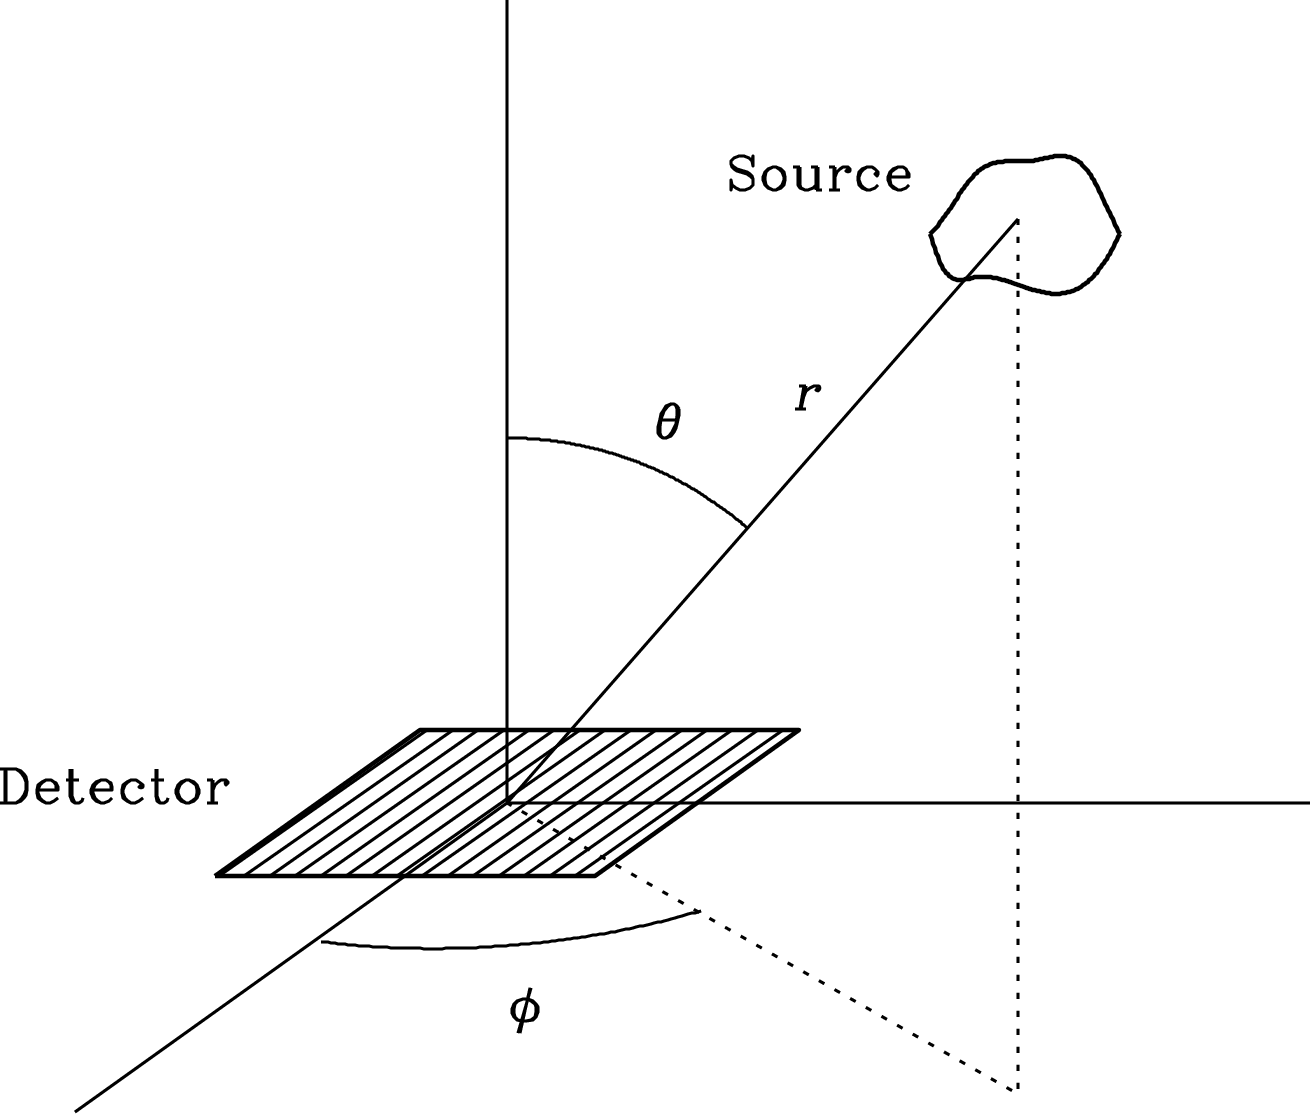
\includegraphics[width=0.5\textwidth]{flux-density}
  \bicaption[\acl*{S-nu} \acs*{S-nu} 的定义示意图]{%
    \acl*{S-nu} \acs*{S-nu} 的定义示意图.
  }{%
    An illustration of the definition of flux density \acs*{S-nu}.
    \\\textcopyright{}
    \citeay{condon2016}, \S\,2.1.
  }
  \label{fig:flux-density}
\end{figure}

对于一个离散源,其所张的立体角是确定的,如图\autoref{fig:flux-density} 所示,
因此探测器单位投影面积上接收到的谱功率 (spectral power)
即为这个源的\emph{\acf{S-nu}}:
\begin{equation}
  \label{eq:flux-density}
  \acs{S-nu} \equiv
    \int_{\R{source}} \acs{I-nu}(\theta,\phi) \cos\theta \,\D{\Omega} ,
\end{equation}
其单位是 [\si{\watt\per\square\meter\per\hertz}].
实际中常用的单位是 \si{\jansky},换算关系为
$\SI{1}{\jansky} = \SI{e-26}{\watt\per\square\meter\per\hertz}$.

\begin{figure}[htp]
  \centering
  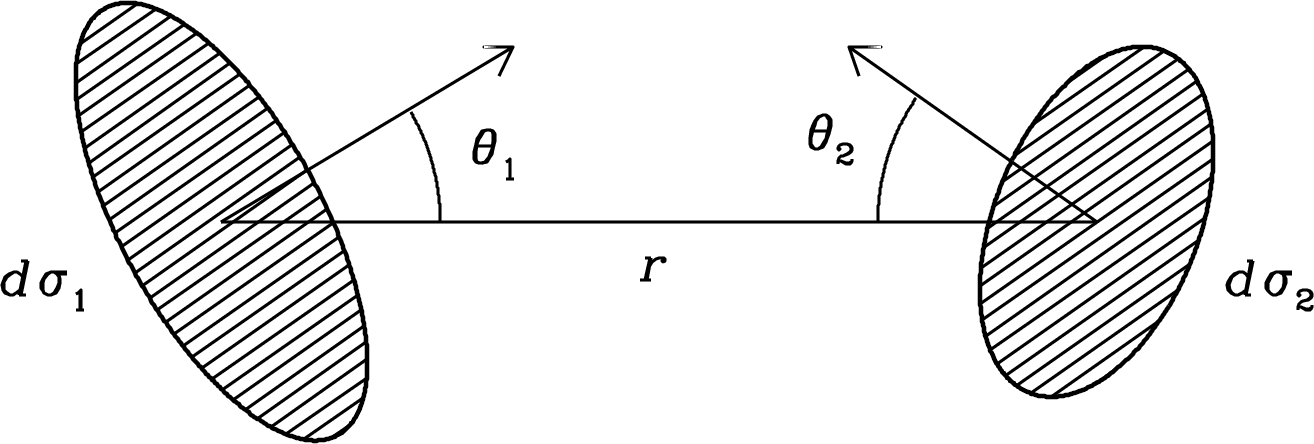
\includegraphics[width=0.6\textwidth]{specific-intensity-conservation}
  \bicaption[\acl*{I-nu} \acs*{I-nu} 沿光线保持不变]{%
    在自由空间里\acl*{I-nu} \acs*{I-nu} 沿光线保持不变.
  }{%
    The specific intensity \acs*{I-nu} conserved along a ray in empty space.
    \\\textcopyright{}
    \citeay{condon2016}, \S\,2.1.
  }
  \label{fig:intensity-conservation}
\end{figure}

考虑由源发射的一束光线,
设 $\D{\sigma_1}$ 和 $\D{\sigma_2}$ 是光线上相距为 $r$ 的两个无限小截面,
如\autoref{fig:intensity-conservation} 所示,
则两个面元相互所张的立体角为:
\begin{align}
  \D{\Omega_1} & = \frac{\cos\theta_2 \,\D{\sigma_2}}{r^2} , \\
  \D{\Omega_2} & = \frac{\cos\theta_1 \,\D{\sigma_1}}{r^2} .
\end{align}
于是,在频率范围 $[\nu, \,\nu+\D{\nu}]$ 以及立体角 $\D{\Omega_1}$ 之内
流过面元 $\D{\sigma_1}$ 的功率为:
\begin{align}
  \D{P_1} & = (\acs{I-nu})_1 \cos\theta_1
      \,\D{\Omega_1} \,\D{\sigma_1} \,\D{\nu}  \\
    & = (\acs{I-nu})_1 \left( \frac{\cos\theta_1 \cos\theta_2}{r^2} \right)
      \,\D{\sigma_1} \,\D{\sigma_2} \,\D{\nu} ,
\end{align}
类似地,流过面元 $\D{\sigma_2}$ 的功率为:
\begin{align}
  \D{P_2} & = (\acs{I-nu})_2 \cos\theta_2
      \,\D{\Omega_2} \,\D{\sigma_2} \,\D{\nu}  \\
    & = (\acs{I-nu})_2 \left( \frac{\cos\theta_1 \cos\theta_2}{r^2} \right)
      \,\D{\sigma_1} \,\D{\sigma_2} \,\D{\nu} .
\end{align}
由于在自由空间里(即没有吸收和发射)能量守恒,即 $\D{P_1} \D{t} = \D{P_2} \D{t}$,
可得:
\begin{equation}
  \label{eq:intensity-conservation}
  (\acs{I-nu})_1 = (\acs{I-nu})_2 .
\end{equation}
所以,在自由空间里\acl*{I-nu} \acs*{I-nu} 沿光线保持不变,与距离无关.

%---------------------------------------------------------------------
\subsection{辐射转移}

\begin{figure}[htp]
  \centering
  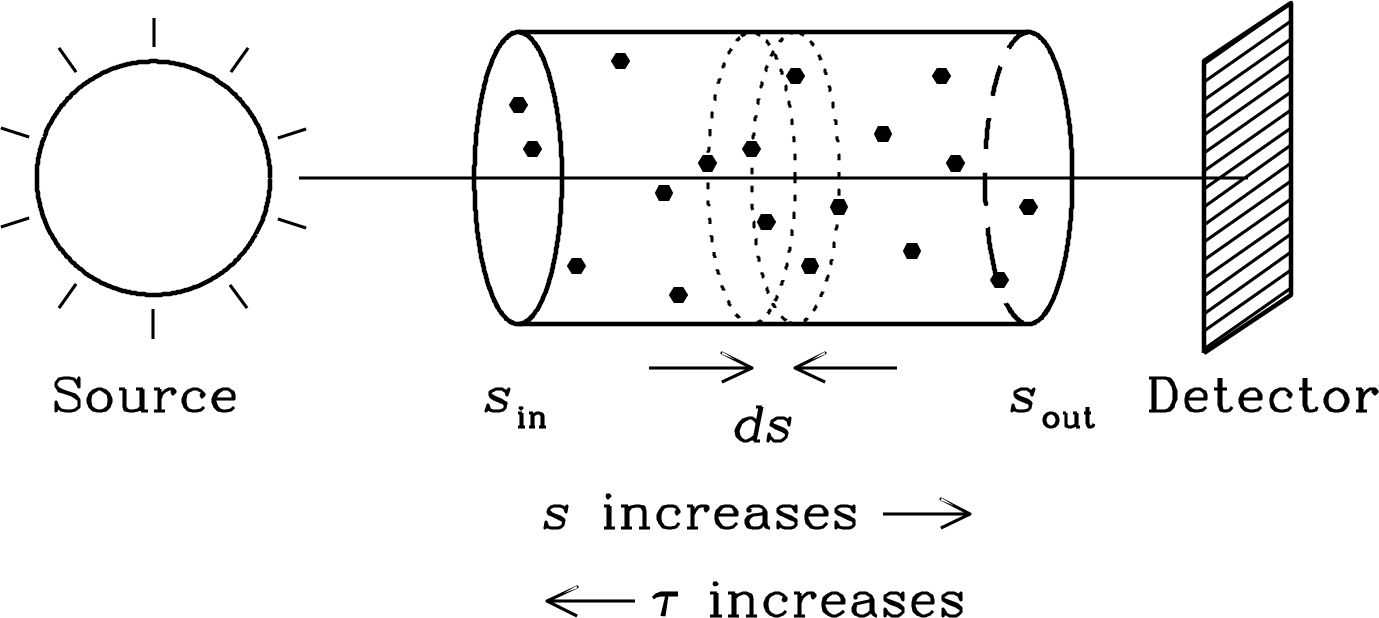
\includegraphics[width=0.6\textwidth]{radiative-transfer}
  \bicaption[辐射转移示意图]{%
    辐射转移示意图.
    距离 $s$ 沿源向探测器的方向增长,介质的入端和出端的距离分别为
    $s_{\R{in}}$ 和 $s_{\R{out}}$.
    光深 $\tau$ 的增长方向与 $s$ 相反.
  }{%
    An illustration of the radiative transfer.
    The distance $s$ increases along the ray from the source to the detector.
    The distances at the input end and the output end of the intervening
    medium are $s_{\R{in}}$ and $s_{\R{out}}$, respectively.
    The optical depth $\tau$ is measured in the opposite direction as $s$.
    \\\textcopyright{}
    \citeay{condon2016}, \S\,2.2.
  }
  \label{fig:radiative-transfer}
\end{figure}

当辐射的传播空间中存在吸收和发射时(如\autoref{fig:radiative-transfer} 所示),
其\acl{I-nu} \acs{I-nu} 会发生改变,具体变化可由\emph{\acf{rt}}方程描述.
首先考虑吸收情形,一个辐射光子通过介质中一个厚度为 $\D{s}$ 的薄层时被吸收的概率 $\D{p}$ 为:
\begin{equation}
  \D{p} = \acs{coef-absorption} \,\D{s} ,
\end{equation}
其中 \acs{coef-absorption} 为\emph{\acl{coef-absorption}},
量纲为 $\big[\text{长度}^{-1}\big]$.
于是,\acl{I-nu} \acs{I-nu} 在通过厚度 $\D{s}$ 的介质后的损失比例为:
\begin{equation}
  \label{eq:rt-absorption}
  \frac{\D{\acs{I-nu}}}{\acs{I-nu}} = - \acs{coef-absorption} \,\D{s} .
\end{equation}
对上式的两边沿介质的吸收路径积分,可得:
\begin{equation}
  \int_{s_{\R{in}}}^{s_{\R{out}}} \frac{\D{\acs{I-nu}}}{\acs{I-nu}}
    = \ln\acs{I-nu} \,\Big|_{s_{\R{in}}}^{s_{\R{out}}}
    = - \int_{s_{\R{in}}}^{s_{\R{out}}} \acs{coef-absorption}(s') \,\D{s'} ,
\end{equation}
即
\begin{equation}
  \label{eq:intensity-loss1}
  \frac{\acs{I-nu}(s_{\R{out}})}{\acs{I-nu}(s_{\R{in}})} =
    \exp \left[ - \int_{s_{\R{in}}}^{s_{\R{out}}}
      \acs{coef-absorption}(s') \,\D{s'} \right] .
\end{equation}
据此,可定义\emph{\acf{optical-depth}}为:
\begin{equation}
  \label{eq:optical-depth}
  \acs{optical-depth} \equiv
    - \int_{s_{\R{out}}}^{s_{\R{in}}} \acs{coef-absorption}(s') \,\D{s'} .
\end{equation}
注意,上式的积分方向与 $s$ 相反(另见\autoref{fig:radiative-transfer}),
如此可使 $\tau > 0$ 并且随着观测者对介质的观测深度而增大.
利用\acl{optical-depth} \acs{optical-depth},
\autoref{eq:intensity-loss1} 可以写成:
\begin{equation}
  \label{eq:intensity-loss}
  \frac{\acs{I-nu}(s_{\R{out}})}{\acs{I-nu}(s_{\R{in}})} =
    \exp (-\acs{optical-depth}) .
\end{equation}
当 $\tau \ll 1$ 时,称介质是\emph{光学薄}的;
当 $\tau \gg 1$ 时,则称介质是\emph{光学厚}的.

另一方面,介质可能产生辐射使\acl{I-nu} \acs{I-nu} 增强.
考虑介质中的一个体积元 $\D{s}\D{\sigma}$,在频率范围 $[\nu, \,\nu+\D{\nu}]$ 内
沿某一方向的立体角元 $\D{\Omega}$ 所发射的谱功率为:
\begin{equation}
  \D{P_{\nu}} =
    \acs{coef-emission} \,\D{s}\,\D{\sigma}\,\D{\nu}\,\D{\Omega} ,
\end{equation}
其中 \acs{coef-emission} 为\emph{\acl{coef-emission} (emission coefficient)}.
当不存在吸收时,\acs{coef-emission} 可表示为:
\begin{equation}
  \label{eq:coef-emission}
  \acs{coef-emission} = \diff{\acs{I-nu}}{s} .
\end{equation}
易知 \acs{coef-emission} 的单位为
[\si{\watt\per\cubic\meter\per\hertz\per\steradian}].
综合上式和\autoref{eq:rt-absorption},可得\emph{\ac{rt}方程}为:
\begin{equation}
  \label{eq:radiative-transfer}
  \diff{\acs{I-nu}}{s} =
    - \acs{coef-absorption} \,\acs{I-nu} + \acs{coef-emission} .
\end{equation}

%---------------------------------------------------------------------
\subsection{黑体辐射和亮温度}

\emph{黑体}是能够吸收全部入射辐射的理想物体.
处于热力学平衡态的黑体产生的辐射称为\emph{黑体辐射},其能谱分布只取决于黑体的温度,
由 \emph{Planck 辐射定律}给出:
\begin{equation}
  \label{eq:planck}
  B_{\nu}(\nu, T) = \frac{2 h \nu^3}{c^2}
    \frac{1}{\exp(h \nu / \acs{kb} T) - 1} ,
\end{equation}
其中 $B_{\nu}$ 是在频率 $\nu$ 处的谱亮度,$h$ 是 Planck 常数,$c$ 是光速.

在射电波段,$h\nu \ll \acs{kb}T$ 通常成立,因此上式可近似为:
\begin{equation}
  \label{eq:rj-approx}
  B_{\nu}(\nu, T) \approx \frac{2\,\acs{kb}T \nu^2}{c^2} .
\end{equation}
该式就是 \emph{Rayleigh--Jeans 近似}.
在该近似下,辐射黑体的谱亮度 $B_{\nu}$ 与其温度 $T$ 严格成正比.
因此,一个源的谱亮度(即比强度) $I_{\nu}$
可以很方便地使用\emph{\acf{T-b}} 来描述:
\begin{equation}
  \label{eq:Tb}
  \acs{T-b}(\nu) \equiv \frac{\acs{I-nu} c^2}{2 \,\acs{kb} \nu^2} .
\end{equation}
注意 \acs{T-b} 会随频率而变.

%---------------------------------------------------------------------
\subsection{电阻的热噪声}

一个温度为 $T$ 的电阻 (resistor),因其内部的载流子(通常是电子)的随机热运动而产生噪声,
该噪声亦称 \emph{Johnson--Nyquist 噪声} \cite{johnson1928,nyquist1928},
其谱功率 (spectral power, 即每单位频率的功率) 由以下 \emph{Nyquist 近似}给出
[详见 \citeay{condon2016}, \S\,2.5]:
\begin{equation}
  \label{eq:nyquist-approx}
  P_{\nu} = \acs{kb} T .
\end{equation}
该式是 Rayleigh--Jeans 近似 [\autoref{eq:rj-approx}] 在电学里的对应.
类似地,该近似公式只适用于 $h\nu \ll \acs{kb}T$ 的经典范畴.
在考虑量子化修正后,严格的 \emph{Nyquist 公式}为:
\begin{equation}
  \label{eq:nyquist}
  P_{\nu} = \frac{h\nu}{\exp(h \nu / \acs{kb} T) - 1} .
\end{equation}


%=====================================================================
\section{天线基础}
\label{sec:antenna}

\emph{天线}可分为接收型(如射电望远镜)和发射型(如雷达)两类.
前者接收外界的电磁波将其转换成电信号,后者则将输入的电信号转换成电磁波发射出去.
在种类繁多的天线中,\emph{短偶极天线}是其中最基本的一种,
下文对其进行简要介绍,并以此天线为例介绍若干重要的天线概念.

%---------------------------------------------------------------------
\subsection{短偶极天线}

\emph{短偶极天线}由两个总长度 $l$ 远小于一个波长 $\lambda$ 的导体组成,
如\autoref{fig:short-dipole} 所示.
当接上一个交流驱动电流后,导体内的电子会发生往复的加速运动,从而激发电磁波.

首先考虑一个加速度为 $\dot{v}$ 的电荷 $q$,在距离 $r$ 处产生的切向
(即与 $r$ 的方向垂直)电场强度为 [详见 \citeay{condon2016}, \S\,2.7]:
\begin{equation}
  \label{eq:q-efield}
  E_{\bot} = \frac{q \dot{v} \sin\theta}{r c^2} ,
\end{equation}
其中 $\theta$ 为 $r$ 与 $v$ 之间的夹角.
天线的每一小段 $\D{z}$ 均会贡献一定的电场强度 $\D{E_{\bot}}$,
由于 $l \ll \lambda$,因此产生的电场总强度为:
\begin{equation}
  \label{eq:dipole-efield1}
  E_{\bot} = \int_{-l/2}^{l/2}
    \frac{\dot{v} \sin\theta}{r c^2} \,\diff{q}{z}\D{z} .
\end{equation}
对于远场情形 ($r \gg l$),$1/r$ 可视为常数而提出积分号.
考虑一个正弦的驱动电流:
\begin{equation}
  \label{eq:dipole-current}
  I = I_0 \Ce^{-\Ci \omega t} ,
\end{equation}
其中 $I_0$ 为电流峰值,
可知 $\dot{v} = -\Ci \omega v$.
利用导线中的电流可表示为:
\begin{equation}
  \label{eq:wire-current}
  I \equiv \diff{q}{t} = \diff{q}{z} \diff{z}{t} = \diff{q}{z} v ,
\end{equation}
可得
\begin{equation}
  \label{eq:dipole-efield2}
  E_{\bot}
    = -\frac{\Ci\omega \sin\theta}{r c^2}
      \int_{-l/2}^{l/2} \diff{q}{z} v \,\D{z}
    = -\frac{\Ci\omega \sin\theta}{r c^2} \int_{-l/2}^{l/2} I\,\D{z} .
\end{equation}
从天线的中点到两端,电流近似线性地减小至 0,即
\begin{equation}
  \label{eq:dipole-current-dist}
  I(z) \approx I_0 \Ce^{-\Ci\omega t}
    \left[ 1 - \frac{|z|}{l/2} \right] .
\end{equation}
最终可得天线在 $r$ 处产生的切向电场强度为:
\begin{equation}
  \label{eq:dipole-efield}
  E_{\bot} \approx
    -\frac{\Ci\omega \sin\theta}{r c^2} \frac{I_0 l}{2} \Ce^{-\Ci\omega t}
    = -\frac{\Ci\Cpi \sin\theta}{c} \frac{I_0 l}{\lambda}
      \frac{\Ce^{-\Ci\omega t}}{r} .
\end{equation}
\autoref{fig:dipole-radiation} 显示了一个无限短的偶极天线(即 Hertz 偶极子)
的电场强度分布图.

\begin{figure}[htp]
  \centering
  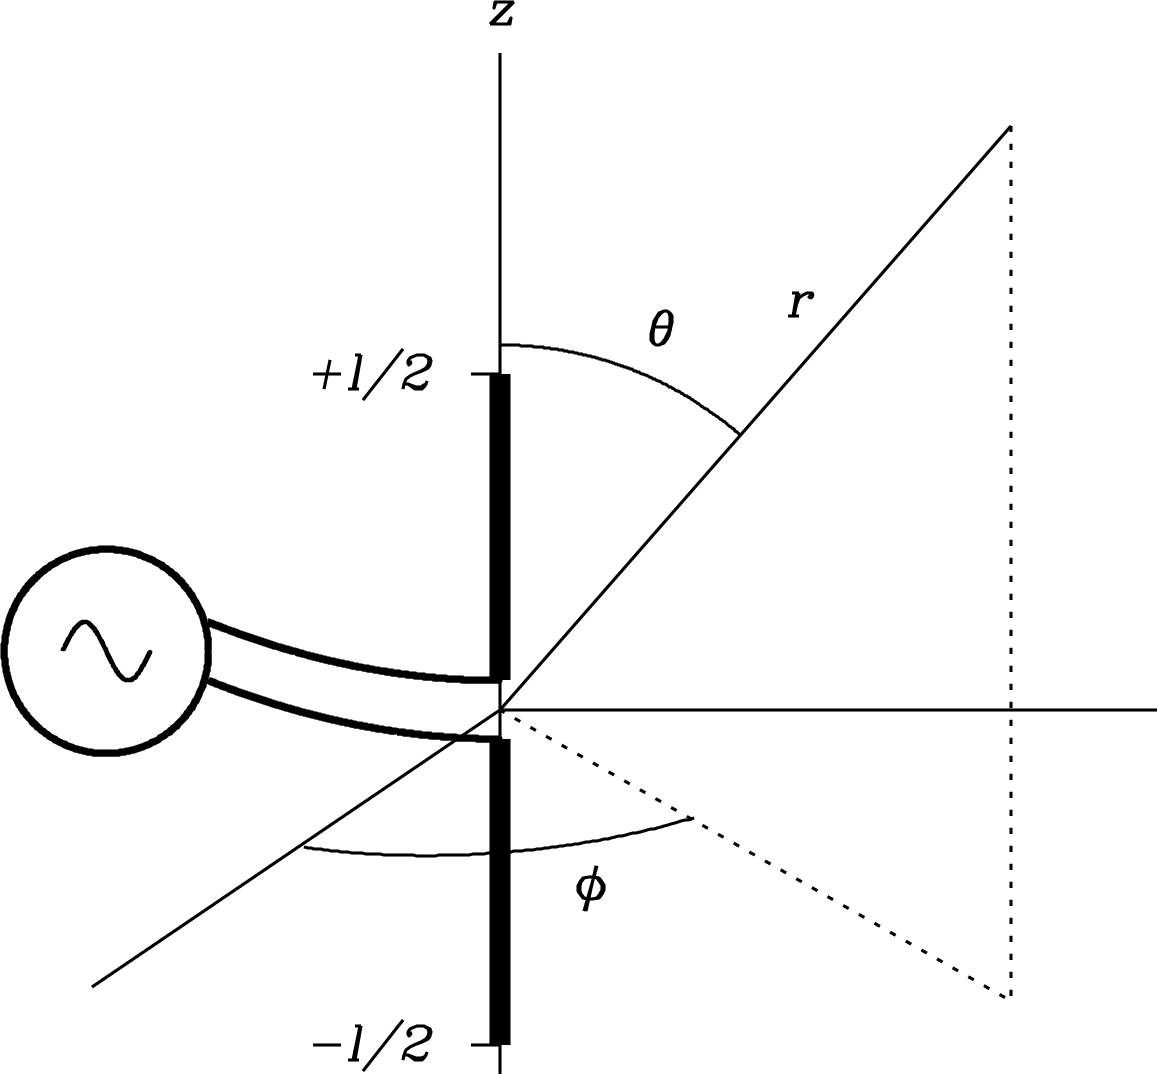
\includegraphics[width=0.5\textwidth]{short-dipole}
  \bicaption[短偶极天线示意图]{%
    分析短偶极天线的辐射所采用的坐标系统.
  }{%
    The coordinate system used to describe the radiation from a
    short dipole.
    \\\textcopyright{}
    \citeay{condon2016}, \S\,3.1.1.
  }
  \label{fig:short-dipole}
\end{figure}

\begin{figure}[htp]
  \centering
  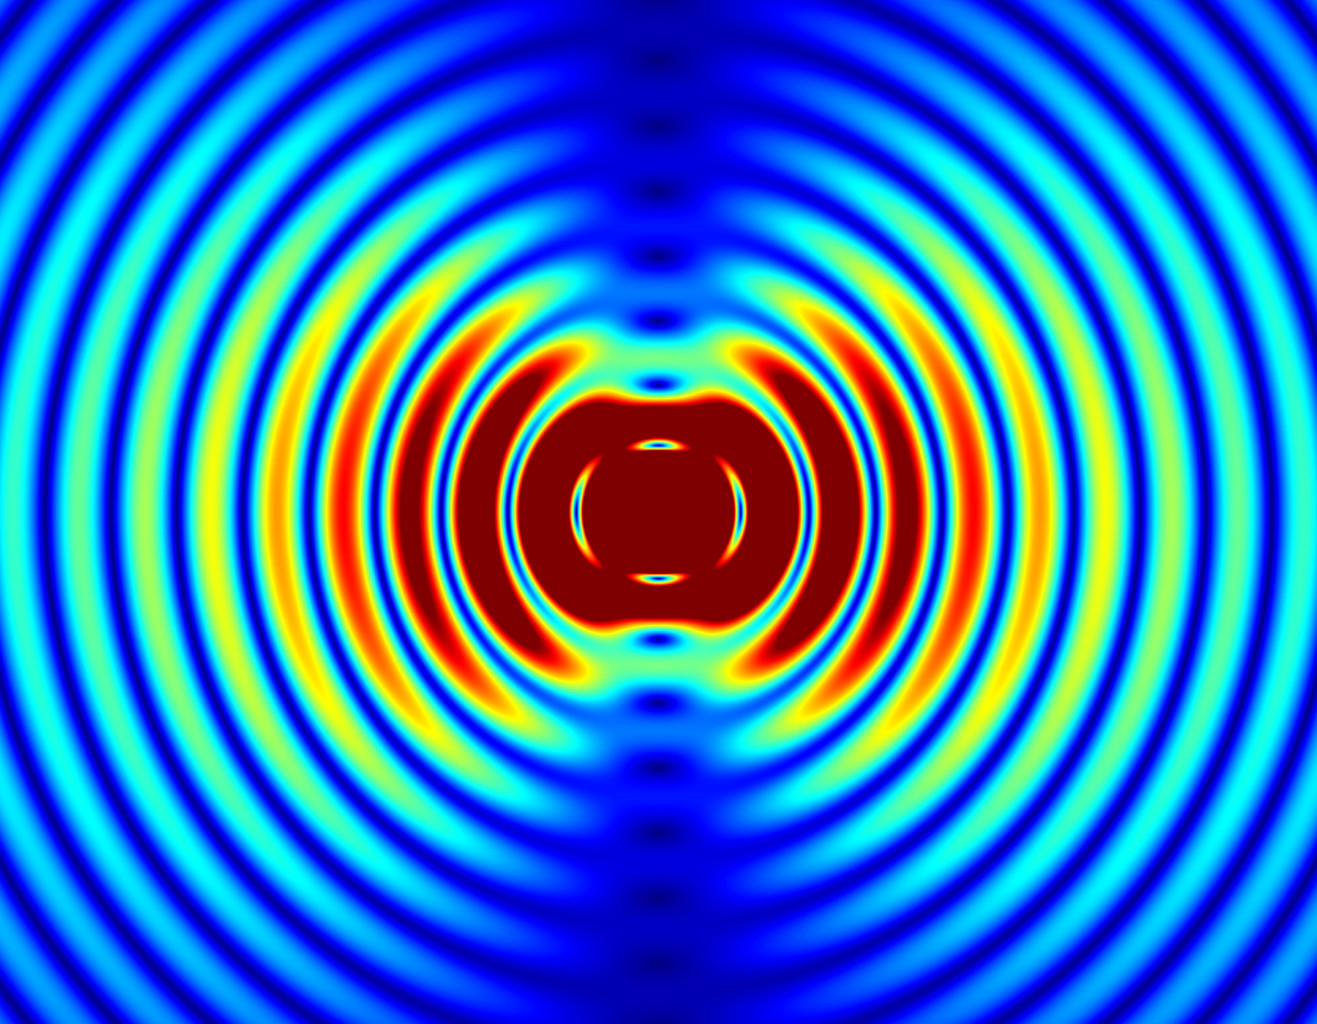
\includegraphics[width=0.6\textwidth]{hertzian-dipole-radiation}
  \bicaption[Hertz 偶极子的电场强度分布图]{%
    Hertz 偶极子的电场强度分布图.
  }{%
    The electric field intensity radiated from a Hertzian dipole.
    \\\textcopyright{}
    nageljr, \url{https://www.deviantart.com/nageljr/art/The-Hertzian-Dipole-Antenna-542377463}, (2019-03-18), CC BY.
  }
  \label{fig:dipole-radiation}
\end{figure}

%---------------------------------------------------------------------
\subsection{功率方向图和增益}

\emph{\acf{pp}} $P(\theta,\phi)$ 是指一个天线的辐射功率的角向分布.
对于短偶极天线,由\autoref{eq:dipole-efield} 可得时间平均的 Poynting 流量
(即单位面积流过的功率)为:
\begin{equation}
  \label{eq:poynting-flux}
  \langle S \rangle = \frac{c}{4\Cpi} \langle E_{\bot}^2 \rangle
    = \frac{\Cpi}{8\,c} \left( \frac{I_0 l}{\lambda} \right)^2
      \frac{\sin^2\theta}{r^2} .
\end{equation}
于是,归一化的\ac{pp}为:
\begin{equation}
  \label{eq:power-pattern}
  P(\theta,\phi) = \sin^2\theta .
\end{equation}
对于更普遍的情况,$P(\theta,\phi)$ 将与两个空间方位角 $(\theta, \phi)$
均相关.

\emph{\acf{gain}} $G(\theta,\phi)$ 定义为天线在方向 $(\theta, \phi)$
的辐射功率 $P(\theta,\phi)$ 与一个总辐射功率相等但各向辐射同性的天线的辐射功率
$\overline{P}$ 之比,即:
\begin{equation}
  \label{eq:gain}
  G(\theta,\phi) = \frac{P(\theta,\phi)}{\overline{P}}
    = \frac{4\Cpi P(\theta,\phi)}{\int P(\theta,\phi) \,\D{\Omega}} .
\end{equation}
可见,一个天线的\ac{gain}与其\ac{pp}只相差一个常数.

%---------------------------------------------------------------------
\subsection{主瓣}

天线的\ac{pp} $P(\theta,\phi)$ 通常会在一定方向范围明显大于在其他方向的值,
这个方向范围便称为天线的\emph{\acf{mainlobe}},
其余的称为\emph{\acf{sidelobe}},如\autoref{fig:lobes} 所示.
主瓣的立体角 $\Omega_{\R{MB}}$ 定义为:
\begin{equation}
  \label{eq:omega-mb}
  \Omega_{\R{MB}} = \int_{\R{MB}} P_n(\theta,\phi) \,\D{\Omega} ,
\end{equation}
其中 $P_n(\theta,\phi) \equiv P(\theta,\phi) / P_{\R{max}}$
为归一化的\ac{pp}.
主瓣的角度范围一般由\emph{\acf{hpbw}}描述,其定义为 $P(\theta,\phi)$
下降至最大值的一半时主瓣的两点之间的角距离,亦如\autoref{fig:lobes} 所示.

\begin{figure}[htp]
  \centering
  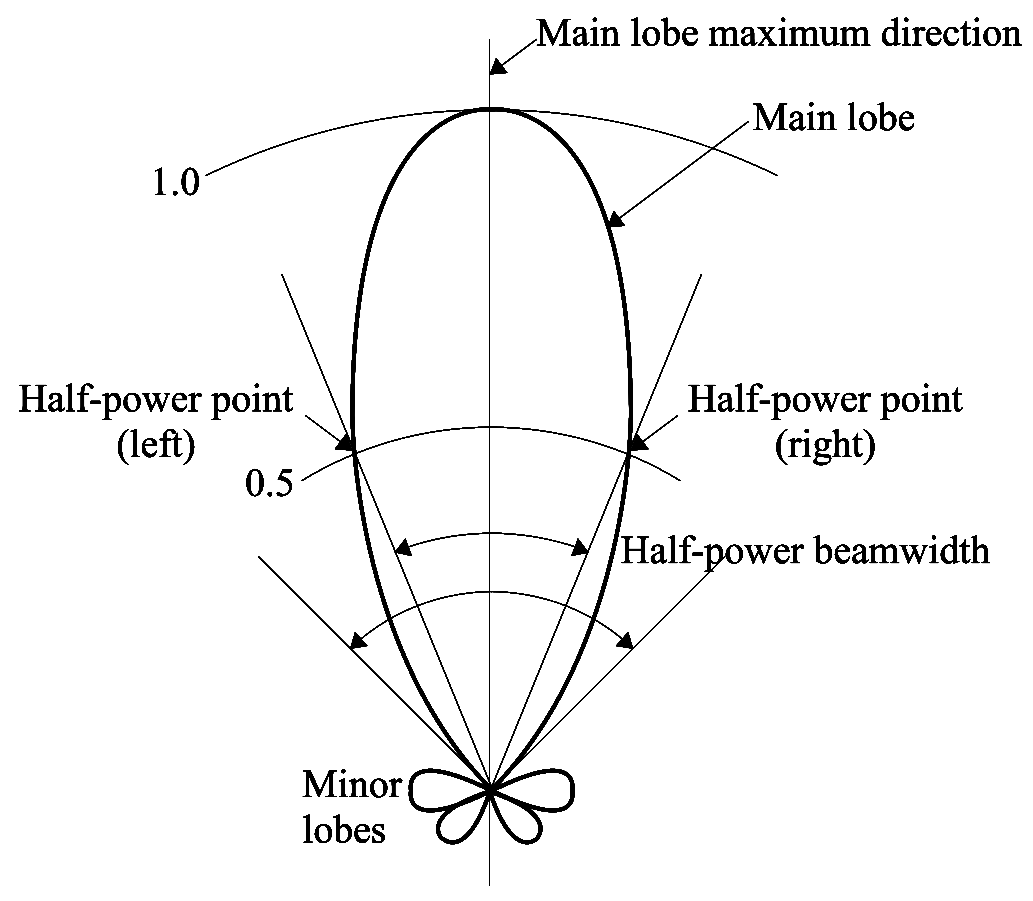
\includegraphics[width=0.6\textwidth]{antenna-lobes}
  \bicaption[天线的主瓣及其宽度示意图]{%
    天线的主瓣及其\acl*{hpbw}示意图.
  }{%
    Diagram of an antenna's main lobe and its HPBW.
    \\\textcopyright{}
    \citeay{zuniga2009}.
  }
  \label{fig:lobes}
\end{figure}

%---------------------------------------------------------------------
\subsection{有效接收面积}

若一个天线测量一个流量密度为 $S_{\nu}$ 的非偏振源输出的谱功率为 $P_{\nu}$,
则该天线的\emph{有效接收面积 (effective collecting area)} $A_e$ 定义为:
\begin{equation}
  \label{eq:area-eff}
  A_e \equiv \frac{2 P_{\nu}}{S_{\nu}} ,
\end{equation}
其中的因子 2 是因为单个天线只能响应一个偏振方向.

\begin{figure}[htp]
  \centering
  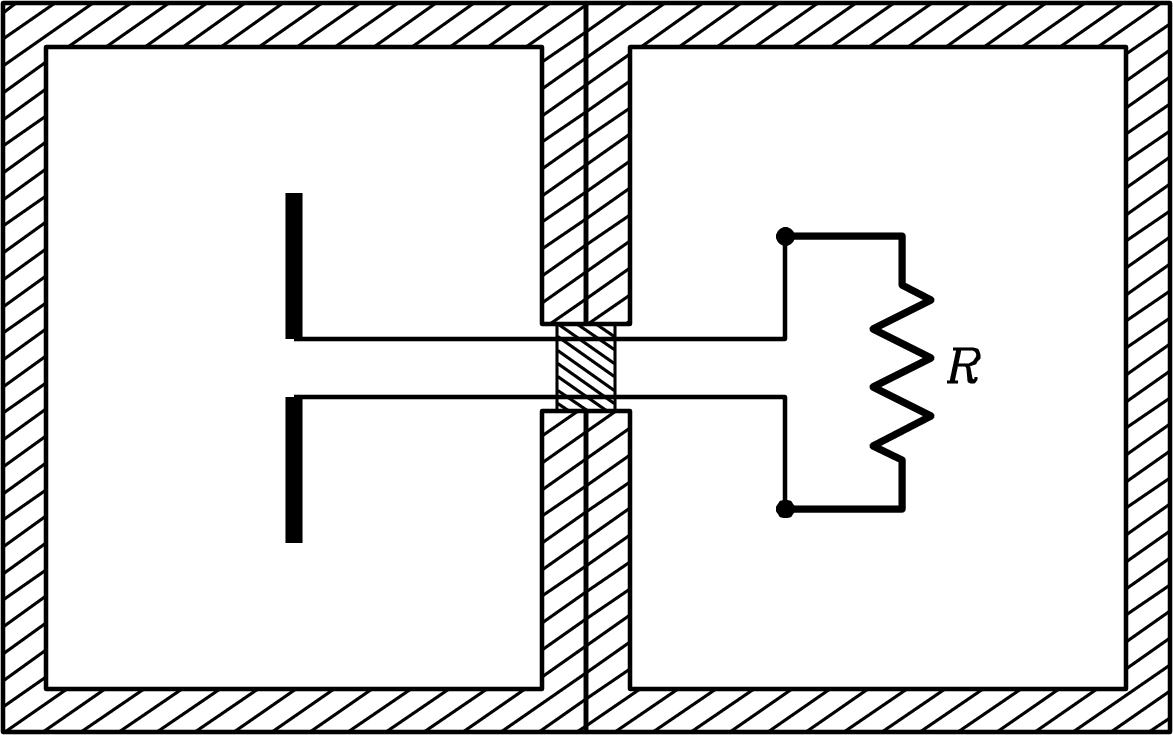
\includegraphics[width=0.5\textwidth]{average-area-thought-exp}
  \bicaption[计算天线平均接收面积的思想实验]{%
    计算天线平均接收面积 $\langle A_e \rangle$ 的思想实验.
  }{%
    A though experiment to calculate the average collection area
    $\langle A_e \rangle$.
    \\\textcopyright{}
    \citeay{condon2016}, \S\,3.1.4.
  }
  \label{fig:Aavg-thought-exp}
\end{figure}

一个天线的\emph{平均接收面积}为:
\begin{equation}
  \label{eq:area-avg1}
  \langle A_e \rangle
    \equiv \frac{1}{4\Cpi} \int A_e(\theta,\phi) \,\D{\Omega} .
\end{equation}
为计算该面积,可借助这样一个思想实验:
一个理想的无损天线和一个匹配的理想电阻,分别置于两个温度均为 $T$ 的空腔中而达到热平衡,
天线和电阻之间使用导线相连,两个空腔之间有一个特殊的阀门,能够阻挡电磁波,
但允许频率范围为 $[\nu, \,\nu+\D{\nu}]$ 的电流通过导线,
如\autoref{fig:Aavg-thought-exp} 所示.
因为整个系统处于热平衡状态,所以导线中没有净能量流动,
否则其中一个空腔将升温、另一个则冷却,违背热力学第二定律.
因此,天线接收各方向的无偏振黑体辐射所产生的总谱功率为:
\begin{equation}
  P_{\nu,a} = \frac{1}{2} \int A_e(\theta,\phi) B_{\nu} \,\D{\Omega} ,
\end{equation}
该谱功率必须等于电阻产生的热噪声的谱功率 $P_{\nu,r}$.
代入\autoref{eq:nyquist} 和\autoref{eq:planck},可得
\begin{equation}
  \acs{kb}T = \frac{2\,\acs{kb}T}{2\lambda^2}
    \int A_e(\theta,\phi) \,\D{\Omega} .
\end{equation}
于是获得天线的平均接收面积 $\langle A_e \rangle$ 为:
\begin{equation}
  \label{eq:area-avg}
  \langle A_e \rangle = \frac{\lambda^2}{4\Cpi}.
\end{equation}

%---------------------------------------------------------------------
\subsection{天线温度}
\label{sec:t-ant}

一个被置于温度为 $T$ 的黑体辐射环境中的天线,
输出的噪声将与温度为 $T$ 的电阻所产生的热噪声 [\autoref{eq:nyquist-approx}]
是不可分辨的,该电阻被称为天线的\emph{匹配电阻}.
据此,可定义\emph{\ac{T-ant}} 为其匹配电阻的温度,即
\begin{equation}
  \label{eq:t-ant}
  \acs{T-ant} \equiv \frac{P_{\nu}}{\acs{kb}} .
\end{equation}
结合\autoref{eq:area-eff} 给出的有效接收面积,
一个流量密度为 $S_{\nu}$ 无偏振辐射源将使天线温度 \acs{T-ant} 上升:
\begin{equation}
  \label{eq:dt-source}
  \Delta T = \frac{A_e S_{\nu}}{2\,\acs{kb}} .
\end{equation}


%=====================================================================
\section{干涉测量原理}
\label{sec:interferometry}

根据衍射原理,望远镜的角分辨率为 $\theta \sim \lambda / D$,
其中 $\lambda$ 为辐射信号的波长(对应于观测频率),$D$ 为望远镜的直径.
相比光学波段,射电信号的波长要长得多,为了实现足够好的角分辨率,
必须建造巨型的望远镜,如 \SI{100}{\meter} 口径的 \ac{gbt}、
\SI{305}{\meter} 口径的 Arecibo、
\SI{500}{\meter} 口径的 \ac{fast}.
然而,在数百 \si{\MHz} 的低频射电波段,望远镜的口径需达到惊人的 \SI{10}{\km}
才能在 \SI{100}{\MHz} 实现约 \SI{1}{\arcminute} 的角分辨率,
这对于单口径望远镜而言显然是不现实的.
因此,低频射电观测通常使用\emph{干涉测量}技术,通过联合一系列小望远镜开展相干测量并综合,
获得高分辨率图像.

%---------------------------------------------------------------------
\subsection{二元准单色干涉仪}

\begin{figure}[htp]
  \centering
  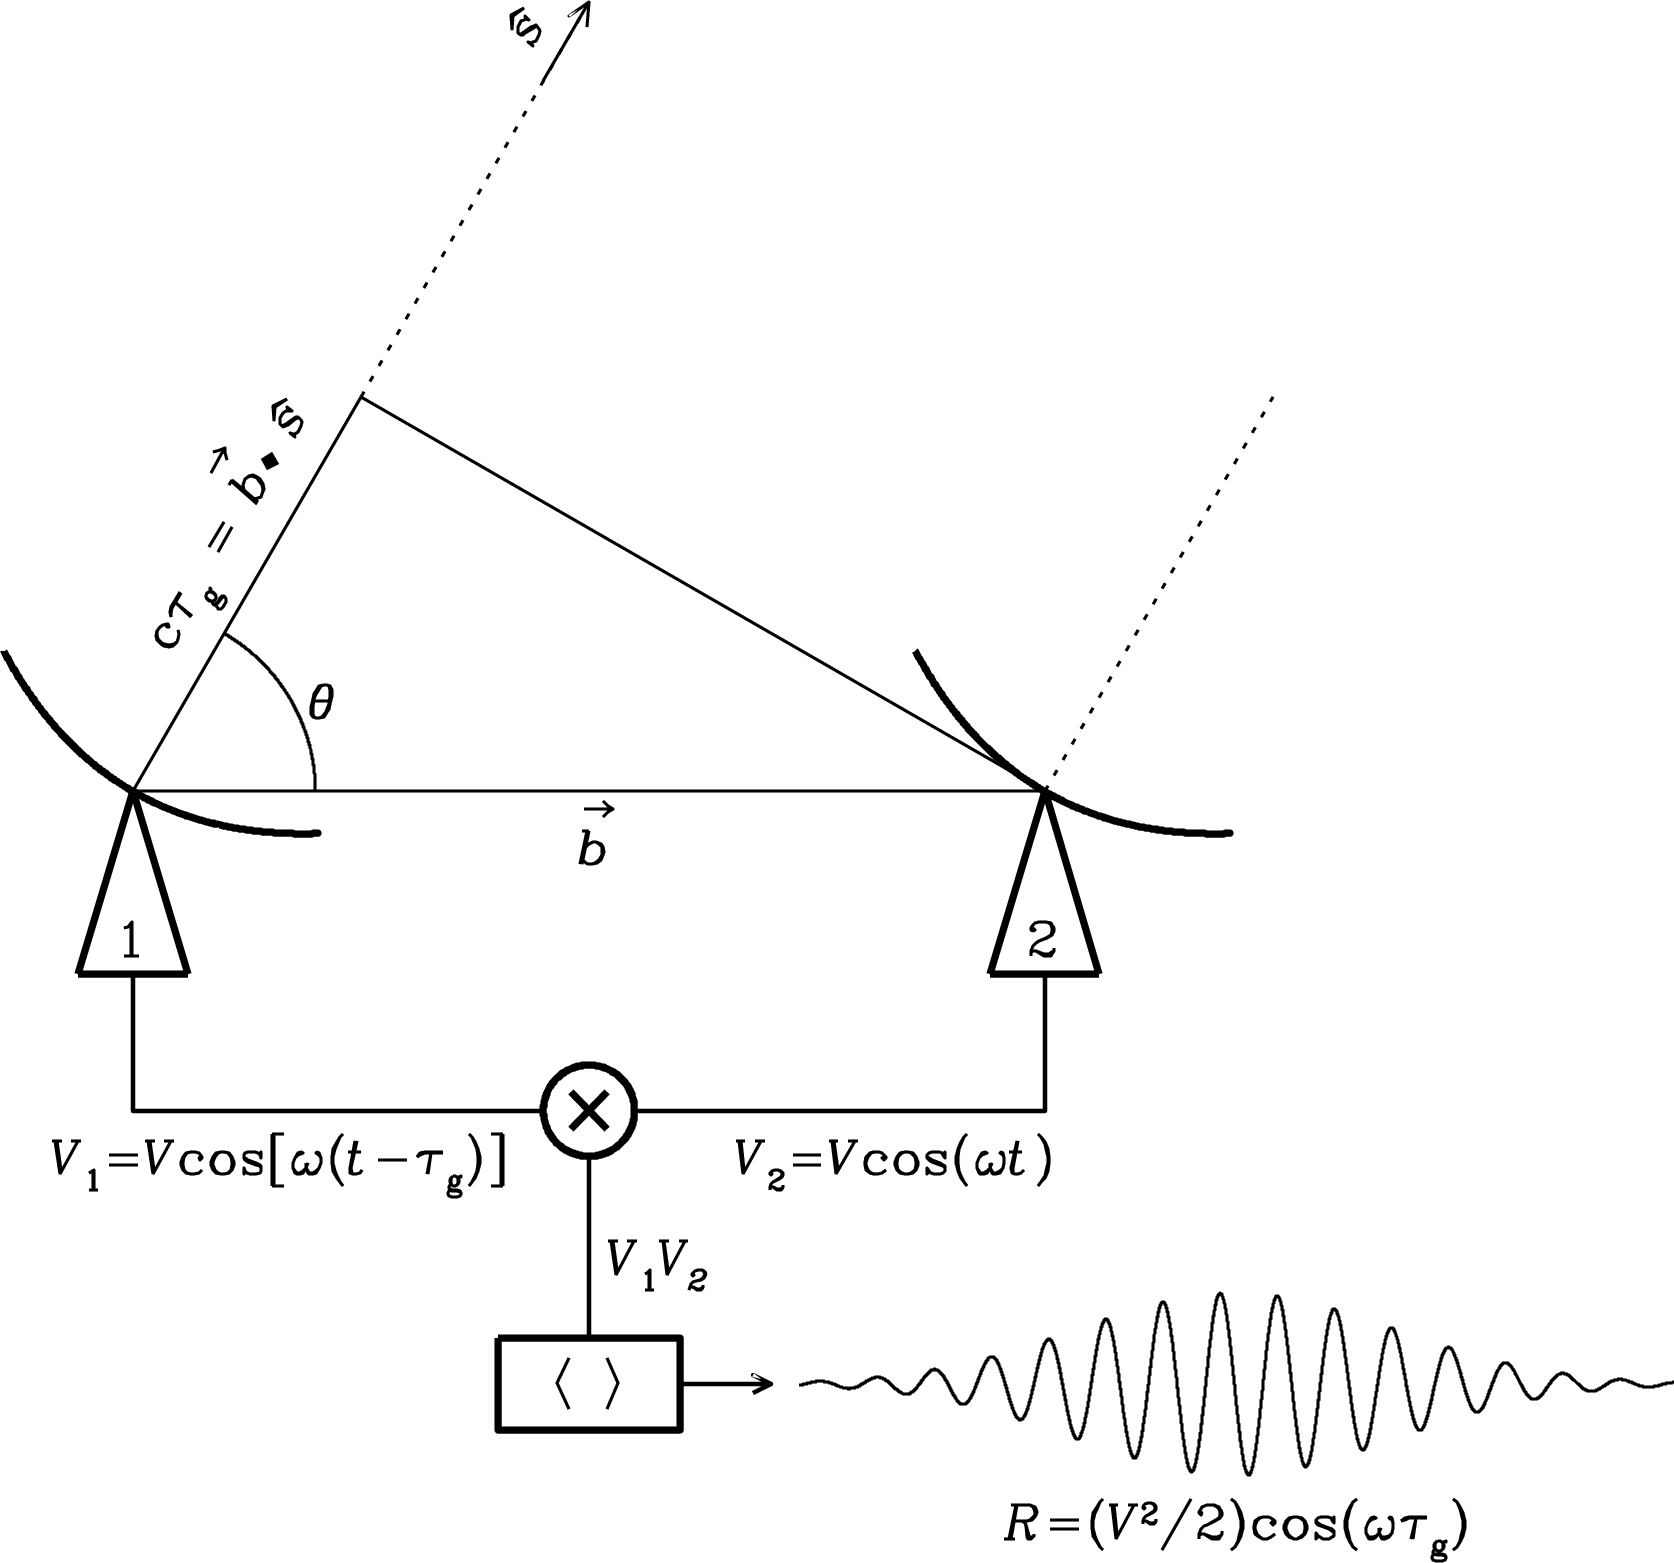
\includegraphics[width=0.7\textwidth]{interferometer}
  \bicaption[二元准单色干涉仪]{%
    二元准单色干涉仪的构成示意图.
    两个相同的天线相距 $\B{b}$ 放置并指向位于 $\hat{\B{s}}$ 方向的辐射源,
    接收的信号被放大后,再经过\acs*{ctor}的相乘($\times$)
    和时间平均($\langle\;\rangle$),得到输出响应 $R$.
  }{%
    The components of a two-element quasi-monochromatic interferometer
    observing in a very narrow radio frequency band centered at
    $\nu = \omega / (2\Cpi)$.
    The two identical antennas are separated by the baseline vector
    $\B{b}$ and point to the source in direction $\hat{\B{s}}$.
    The signals received by the antennas are amplified,
    multiplied ($\times$), and time averaged ($\langle\;\rangle$)
    by the correlator to yield the output response $R$.
    \\\textcopyright{}
    \citeay{condon2016}, \S\,3.7.1.
  }
  \label{fig:interferometer}
\end{figure}

考虑一个最简单的二元准单色干涉仪(如\autoref{fig:interferometer} 所示),
由两个相同的天线和相关器构成,只测量频率为 $\nu$ 的准单色信号.
由于辐射源非常遥远,其信号到达干涉仪时为平面波(忽略电离层扰动等影响).
同一个波面被两个天线接收之间存在一个时间差,即\emph{\acf{tau-g}}:
\begin{equation}
  \label{eq:tau-g}
  \acs{tau-g} = \frac{\B{b} \cdot \hat{\B{s}}}{\acs{c}},
\end{equation}
其中 \acs{c} 是\acl{c},
$\B{b}$ 为两天线之间的基线矢量(由天线 1 指向天线 2),
$\hat{\B{s}}$ 为指向辐射源的单位矢量.
两个天线接收信号后分别输出电压响应:
\begin{align}
  V_1(t) &= V \cos [\omega (t - \acs{tau-g})], \\
  V_2(t) &= V \cos (\omega t),
\end{align}
其中 $\omega = 2\Cpi\nu$ 为角频率.
然后,\emph{\acf{ctor}}将两个天线的响应相乘:
\begin{align}
  V_1(t) V_2(t) &= V^2 \cos [\omega (t - \acs{tau-g})] \cos (\omega t) \\
    &= \frac{1}{2} V^2 \left[ \cos (2\omega t - \omega \acs{tau-g})
      + \cos (\omega \acs{tau-g}) \right].
\end{align}
接着,\ac{ctor}再对相乘后的响应进行时间平均 [参见\autoref{eq:ctor-avgtime}]:
\begin{equation}
  \label{eq:resp-corr}
  R = \langle V_1(t) V_2(t) \rangle
    = \frac{1}{2} V^2 \cos (\omega \acs{tau-g}).
\end{equation}
由于天线响应 $V_1$ 和 $V_2$ 正比于辐射源的电场强度以及天线的\ac{gain}
[参见\autoref{eq:gain}],
因此\ac{ctor}的响应 $R$ 正比于辐射源的流量密度 $S$
以及 $\sqrt{A_1 A_2}$,其中 $A_1$ 和 $A_2$ 为两个天线的有效接收面积
[参见\autoref{eq:area-avg}].

由于地球的自转,辐射源的方向 $\hat{\B{s}}$ 发生变化,\acl{tau-g} \acs{tau-g}
也随之变化,于是\ac{ctor}的输出 $R$ 出现正弦形式的振荡,即\emph{\acf{fringe}},
其相位为:
\begin{equation}
  \phi = \omega\tau_g = 2\Cpi b \cos\theta / \lambda,
\end{equation}
其中 $\theta$ 为方向 $\hat{\B{s}}$ 和基线矢量 $\B{b}$ 之间的夹角.
于是有
\begin{equation}
  \diff{\phi}{\theta} = 2\Cpi \left( \frac{b \sin\theta}{\lambda} \right),
\end{equation}
可得单个\ac{fringe}的宽度,即干涉仪的\emph{\acf{sb-width}}:
\begin{equation}
  \label{eq:sb-width}
  \acs{sb-width} = \frac{\lambda}{b \sin\theta},
\end{equation}
此参数描述了干涉仪的角分辨能力.

天线的\ac{pp}描述了其响应随方向的变化情况,也被称为干涉仪的\emph{\acf{pb}},
将对输出 $R$ 产生调制,如\autoref{fig:interferometer} 所示,
其中\ac{ctor}的输出\ac{fringe}的包络示意了\ac{pb}的衰减情况.

对于一个表面亮度分布为 $\acs{I-nu}(\hat{\B{s}})$ 的\ac{extsrc},
由于不同位置产生的辐射互不相干,因此可以被当作一系列独立的点源处理,
于是上述二元准单色干涉仪的输出响应为:
\begin{equation}
  \label{eq:resp-cos}
  R_c = \int \acs{I-nu}(\hat{\B{s}}) \cos \left(
      \omega \B{b}\cdot\hat{\B{s}} / c \right) \D{\Omega}
    = \int \acs{I-nu}(\hat{\B{s}}) \cos \left(
      2\Cpi\, \B{b}\cdot\hat{\B{s}} / \lambda \right) \D{\Omega},
\end{equation}
其中下标 \enquote{$c$} 表示 \enquote{cosine} \ac{ctor}的输出,
以区分下文将要介绍的 \enquote{sine} \ac{ctor}.

一个任意的亮度分布 $I$ 可分解为奇对称成分 $I_O$ 与偶对称成分 $I_E$ 之和,
然而\autoref{eq:resp-cos} 描述的 cosine \ac{ctor}只能测量其中的
偶对称成分 $I_E$,即:
\begin{equation}
  R_c = \int \left[ I_O(\hat{\B{s}}) + I_E(\hat{\B{s}}) \right]
      \cos \left( 2\Cpi\, \B{b}\cdot\hat{\B{s}} / \lambda \right)
      \D{\Omega}
    = \int I_E(\hat{\B{s}}) \cos \left(
      2\Cpi\, \B{b}\cdot\hat{\B{s}} / \lambda \right) \D{\Omega}.
\end{equation}
为了能够测量另一个奇对称成分 $I_O$,则需要一个 \enquote{sine} \ac{ctor},
可通过对其中一个天线的输出增加 $\Cpi/2$ 的相位延迟来实现,于是有:
\begin{equation}
  R_s = \int \left[ I_O(\hat{\B{s}}) + I_E(\hat{\B{s}}) \right]
      \sin \left( 2\Cpi\, \B{b}\cdot\hat{\B{s}} / \lambda \right)
      \D{\Omega}
    = \int I_O(\hat{\B{s}}) \sin \left(
      2\Cpi\, \B{b}\cdot\hat{\B{s}} / \lambda \right) \D{\Omega}.
\end{equation}
\ac{cctor} 即为一对 cosine 和 sine \ac{ctor}的组合.
相应地,\emph{\acf{Vis}},简称\emph{\ac{vis}},可定义为:
\begin{equation}
  \label{eq:vis}
  \acs{Vis} \equiv R_c - \Ci R_s
    = \int I_{\nu}(\hat{\B{s}}) \exp
      (-2\Cpi\Ci\, \B{b}\cdot\hat{\B{s}} / \lambda) \D{\Omega}.
\end{equation}

%---------------------------------------------------------------------
\subsection{有限带宽}

现在,将上述二元干涉仪推广至测量有限带宽的信号.
考虑一段中心频率为 $\nu_c$ 且宽度为 $\Delta\nu$ 的窄频带,
若辐射源的亮度以及天线的响应在此频带内基本不变,
则可知测量的\ac{vis} [\autoref{eq:vis}] 为:
\begin{align}
  \acs{Vis} &= \int \left[ \frac{1}{\Delta\nu}
        \int_{\nu_c-\Delta\nu/2}^{\nu_c+\Delta\nu/2}
        I(\hat{\B{s}}, \nu) \exp (-2\Cpi\Ci\, \nu\tau_g)
      \right] \D{\Omega} \\
    &\approx \int I_{\nu}(\hat{\B{s}}) \sinc (\Delta\nu\,\tau_g)
      \exp (-2\Cpi\Ci\, \nu_c\tau_g) \D{\Omega},
  \label{eq:vis-bw}
\end{align}
其中 $\sinc(\cdot)$ 为归一化 sinc 函数,定义如下:
\begin{equation}
  \label{eq:sinc}
  \sinc(x) =
    \begin{cases}
      \sin(\Cpi x) / (\Cpi x), & \quad \text{if } x \neq 0, \\
      1, & \quad \text{if } x = 0.
    \end{cases}
\end{equation}
因此,干涉仪测得的\ac{fringe}幅度减弱至原来的 $\sinc(\Delta\nu\,\tau_g)$ 倍.
为了最小化该损失,可以给前导天线的输出信号增加\emph{\acf{tau-c}},
如\autoref{fig:interferometer-tau0} 所示,并随地球自转而调节 \acs{tau-c}
使其满足 $|\acs{tau-c} - \acs{tau-g}| \ll (\Delta\nu)^{-1}$.
在此情况下,到达\ac{ctor}时两个天线的信号的相位是同步的.
同时,满足 $\acs{tau-c} = \acs{tau-g}$ 的方向 $\hat{\B{s}}_0$
称为\emph{\acf{delay-center}}或\emph{\acf{phase-refpos}}.

\begin{figure}[htp]
  \centering
  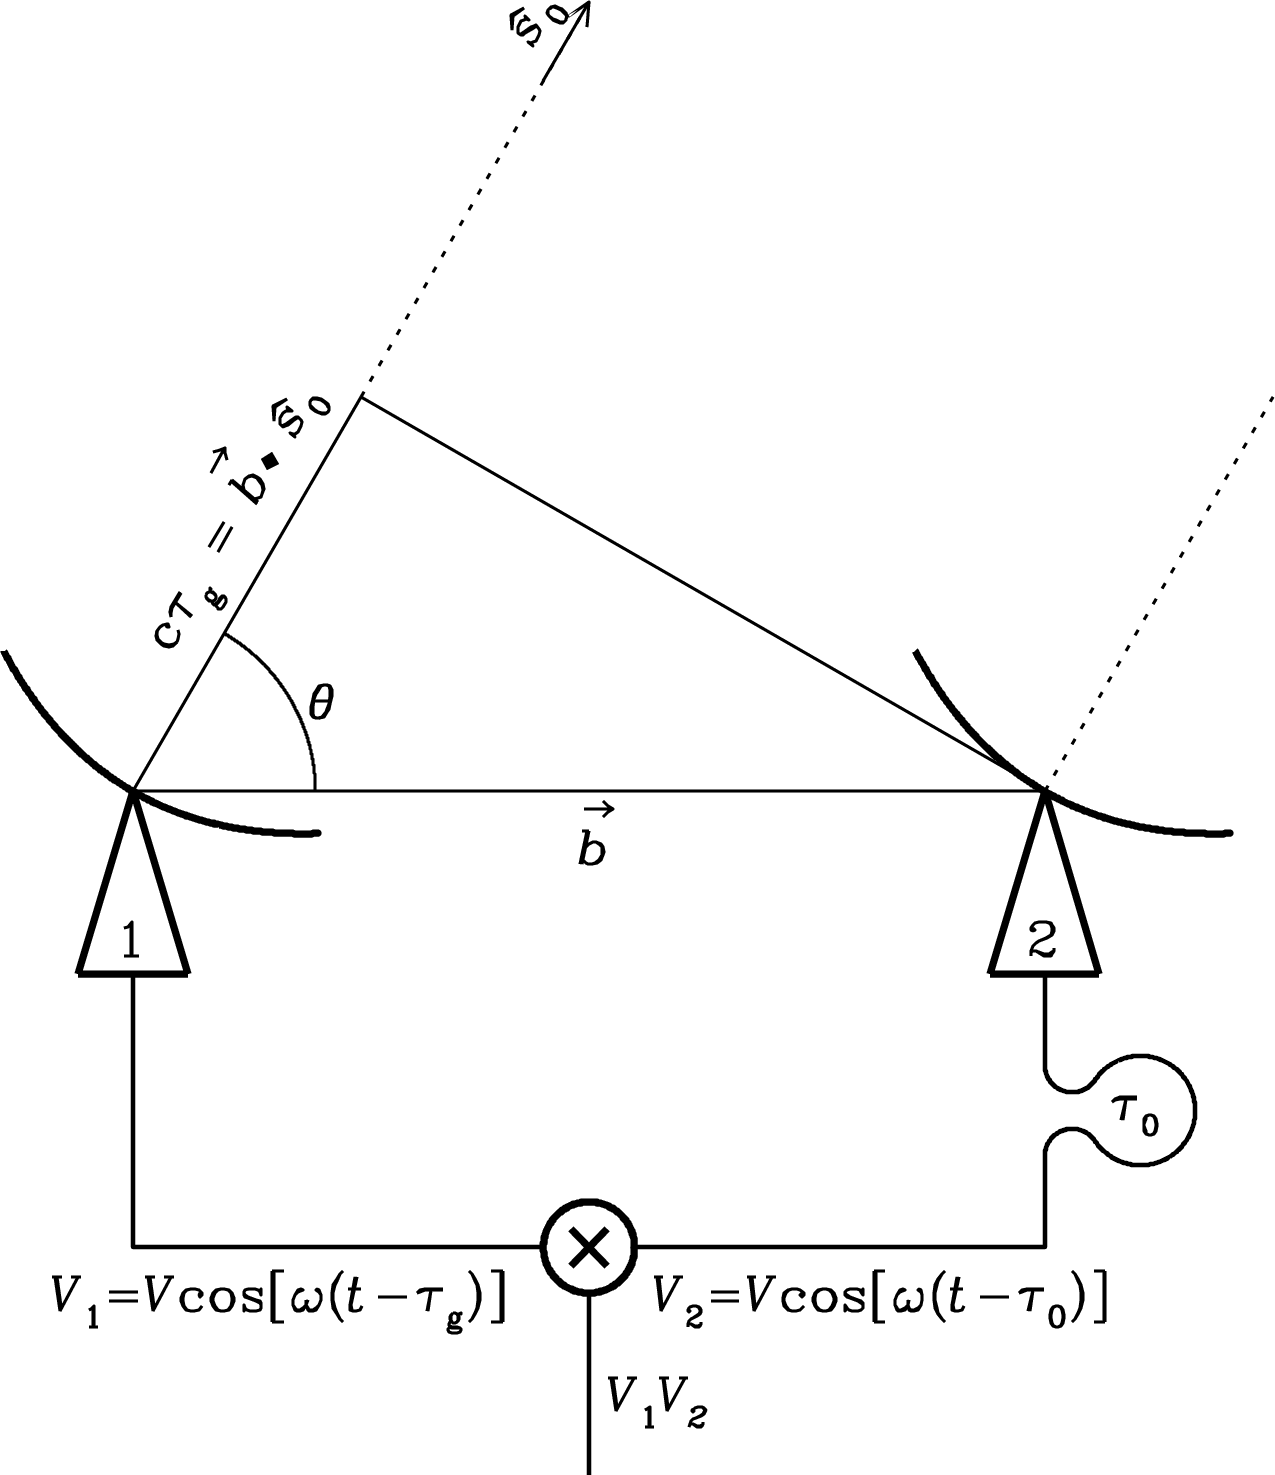
\includegraphics[width=0.6\textwidth]{interferometer-tau0}
  \bicaption[\acl*{tau-c} \acs*{tau-c}]{%
    通过给前导天线(即天线 2)增加\acl*{tau-c}
    $\acs*{tau-c} \approx \acs*{tau-g}$,
    使得两天线的信号在相关运算时相位尽量同步,从而最小化带宽效应对测量条纹的衰减影响.
  }{%
    By introducing the compensating delay
    $\acs*{tau-c} \approx \acs*{tau-g}$ in the signal path of the leading
    antenna (i.e., antenna 2), the phases of the two signals are almost
    in sync when they reach the correlator, hence minimizing the
    attenuation to the measured fringes caused by the finite bandwidth
    effect.
    \\\textcopyright{}
    \citeay{condon2016}, \S\,3.7.3.
  }
  \label{fig:interferometer-tau0}
\end{figure}

\acl{tau-g} \acs{tau-g} 会随方向而变化,因此\acl{tau-c} \acs{tau-c}
只对特定方向 $\hat{\B{s}}_0$ (即\ac{delay-center})是正好准确的.
偏离\ac{delay-center}的角度 $\Delta\theta$ 越大,\acl{tau-c} \acs{tau-c}
的修正效果越差,带宽带来的损失越大,即\emph{\acf{bw-smear}}.
该涂污效应限制了有效的视场大小,为满足:
\begin{equation}
  \Delta\nu \Delta\tau_g
    \approx \Delta\nu \diff{\tau_g}{\theta} \Delta\theta
    = \frac{b \sin\theta}{c} \Delta\nu \Delta\theta
    \ll 1,
\end{equation}
则要求:
\begin{equation}
  \Delta\theta \ll \frac{\nu \acs{sb-width}}{\Delta\nu}.
\end{equation}
另一个解决\ac{bw-smear}的方法是将宽频带划分为一系列足够窄的频率通道
(如每个通道仅宽几十 \si{\kHz}),每个通道的信号都被独立地相关运算得到\ac{vis}.

类似地,如果\ac{ctor}的积分时间 $\Delta t$ 过长,则辐射源的位置 $\hat{\B{s}}$
会因地球自转而发生显著改变(可与 \acs{sb-width} 相比拟),
导致\acl{tau-c} \acs{tau-c} 的修正效果变差,即\emph{\acf{t-smear}}.
一个距离\acl{delay-center} $\Delta\theta$ 的目标的移动速度为
$v = \omega_e \Delta\theta$,其中 $\omega_e$ 为地球自转的角速度.
为了最小化\ac{t-smear}的影响,\ac{ctor}的积分时间 $\Delta t$ 需满足:
\begin{equation}
  v \Delta t = \omega_e \Delta\theta \Delta t \ll \theta_s,
\end{equation}
即:
\begin{equation}
  \label{eq:ctor-avgtime}
  \Delta t \ll \frac{\theta_s}{\omega_e \Delta\theta}.
\end{equation}

%---------------------------------------------------------------------
\subsection{成像原理}

\begin{figure}[htp]
  \centering
  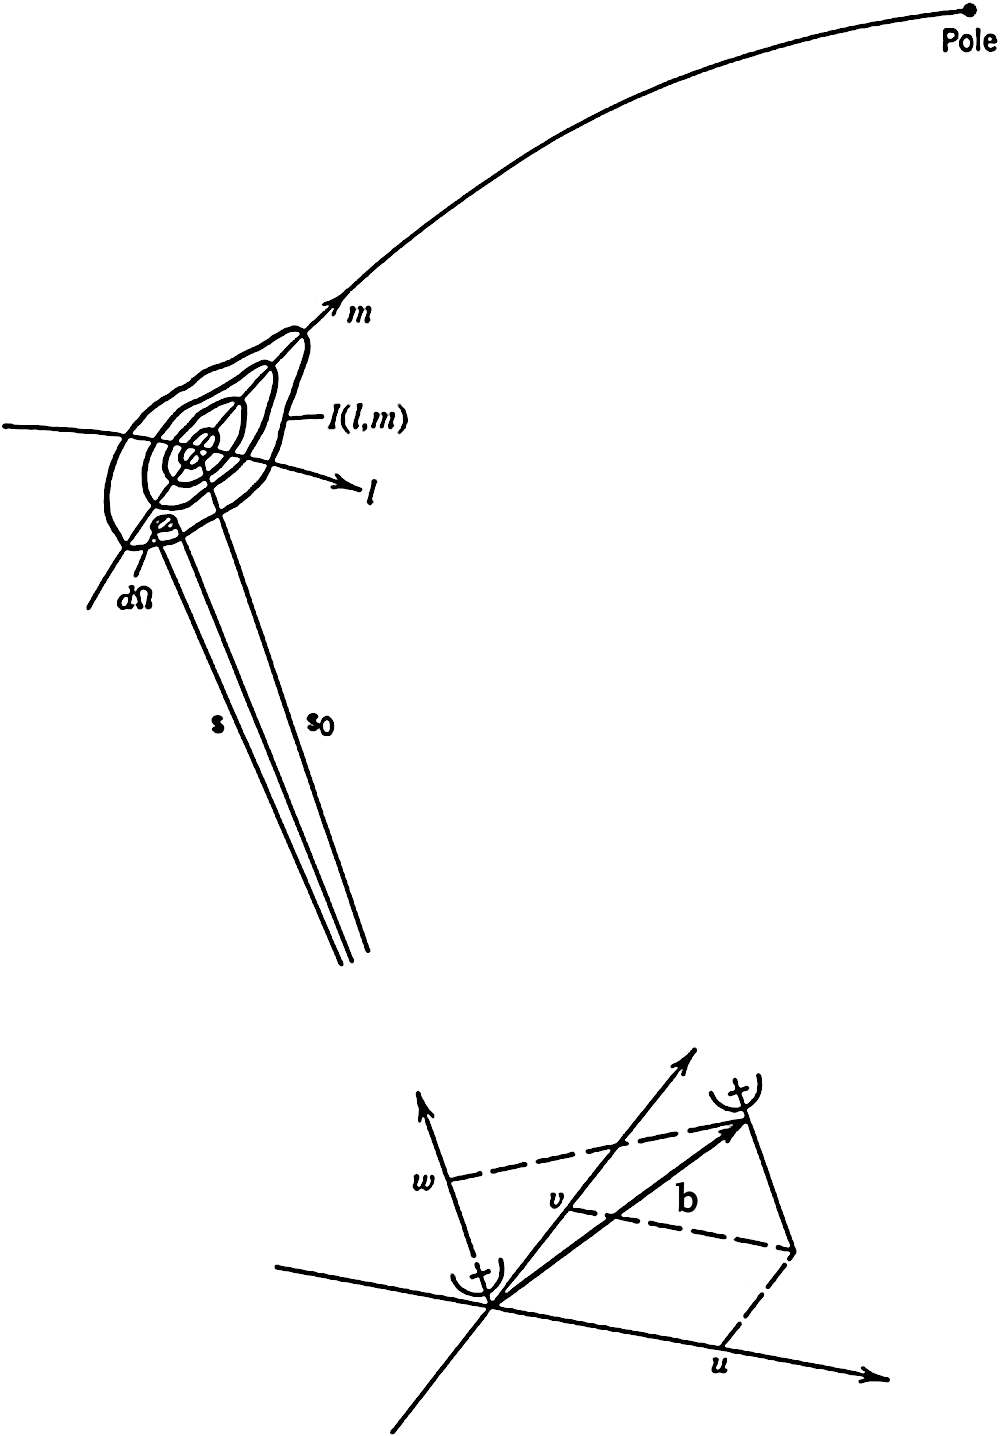
\includegraphics[width=0.7\textwidth]{interferometer-coordsys}
  \bicaption[$(u,v,w)$ 坐标系]{%
    干涉仪的 $(u,v,w)$ 直角坐标系,其中 $w$ 轴指向参考方向 $\hat{\B{s}}_0$,
    通常为目标的中心,$u$ 轴向东,$v$ 轴向北.
    基线矢量可表示为 $\B{b} = (u,v,w) \lambda$,
    目标的亮度分布则用\acs*{dc}描述,即 $I(\hat{\B{s}}) = I(l,m)$,
    其中 $l, m$ 为方向矢量 $\hat{\B{s}}$ 分别对 $u, v$ 轴的投影长度.
  }{%
    The $(u,v,w)$ Cartesian coordinate system for interferometers,
    in which the $w$-axis points in the reference direction
    $\hat{\B{s}}_0$ (usually toward the source center), and
    the $u$- and $v$-axes point east and north, respectively.
    A baseline vector is represented as $\B{b} = (u,v,w) \lambda$,
    and the source brightness distribution is described as
    $I(\hat{\B{s}}) = I(l,m)$, where $l, m$ are direction cosines,
    i.e., the projected lengths of the direction vector $\hat{\B{s}}$
    against the $u$- and $v$-axes, respectively.
    \\\textcopyright{}
    \citeay{thompson2017}, \S\,3.1.
  }
  \label{fig:interferometer-coordsys}
\end{figure}

为了能够实际运用\autoref{eq:vis} 或\autoref{eq:vis-bw} 获得图像,
需要定义一个坐标系,如\autoref{fig:interferometer-coordsys}
所示的 $(u,v,w)$ 直角坐标系是最常用的,其中 $w$ 轴指向参考方向 $\hat{\B{s}}_0$,
通常为目标的中心,$u$ 轴向东,$v$ 轴向北.
于是,基线矢量 $\B{b} = (u,v,w) \lambda$,
方向矢量 $\hat{\B{s}} = \left( l, m, \sqrt{1-l^2-m^2} \right)$,
其中 $l, m$ 为 $\hat{\B{s}}$ 分别对 $u, v$ 轴的投影长度,即\ac{dc}.
再利用 $\D{\Omega} = \D{l}\D{m} \,\big/ \sqrt{1-l^2-m^2}$,
\autoref{eq:vis} 可表示为:
\begin{equation}
  \label{eq:vis-uvw}
  \acs{Vis}(u,v,w) = \iint \frac{I_{\nu}(l,m)}{\sqrt{1-l^2-m^2}}
    \exp \left[ -2\Cpi\Ci \left( ul+vm+w\sqrt{1-l^2-m^2} \right) \right]
    \D{l}\D{m}.
\end{equation}
需注意,这\emph{不是}二维 Fourier 变换.

然而,在下述两种常见的特殊情况下,上式可变成二维 Fourier 变换,
从而通过逆运算获得目标的亮度分布.
\begin{itemize}
\item
\emph{所有基线矢量共面:}
这可进一步分为两种情形:
(1) 干涉阵列的天线只沿东西方向分布,如 \ac{wsrt},尽管地球自转,
所有基线矢量均落在同一垂直于地球自转轴的平面内;
(2) 虽然干涉阵列的天线分布在一个二维平面,如 \autoref{ssec:miteor}
将介绍的 \ac*{miteor},但只考虑瞬时观测.
此时,可以选取合适的坐标系使得 $w = 0$,于是\autoref{eq:vis-uvw}
变成二维 Fourier 变换,利用其逆变换可得目标的亮度分布为:
\begin{equation}
  \label{eq:vis-inv1}
  \frac{I_{\nu}(l,m)}{\sqrt{1-l^2-m^2}} = \iint \acs{Vis}(u,v, w \equiv 0)
    \exp [2\Cpi\Ci\, (ul+vm)] \D{l}\D{m}.
\end{equation}

%.......................................
\item
\emph{小视场成像:}
对于任何干涉阵列,如果只考虑以参考方向 $\hat{\B{s}}_0$ 为中心的足够小的区域,
于是有:
\begin{equation}
  w\sqrt{1-l^2-m^2} \approx w \left[ 1 - \frac{1}{2} (l^2+m^2) \right].
\end{equation}
则\autoref{eq:vis-uvw} 成为:
\begin{equation}
  \acs{Vis}(u,v,w) \approx \exp (-2\Cpi\Ci\,w) \iint
    \frac{I_{\nu}(l,m)}{\sqrt{1-l^2-m^2}}
    \exp [-2\Cpi\Ci\, (ul+vm) -\Ci\Cpi w(l^2+m^2)] \D{l}\D{m}.
\end{equation}
如果 $|\Cpi w(l^2+m^2)| \ll 1$,即 $\exp [-\Ci\Cpi w(l^2+m^2)] \sim 1$,
则上式成为二维 Fourier 变换,即:
\begin{equation}
  \acs{Vis}(u,v) \equiv \acs{Vis}(u,v,w) \exp (2\Cpi\Ci\,w)
    = \iint \frac{I_{\nu}(l,m)}{\sqrt{1-l^2-m^2}}
    \exp [-2\Cpi\Ci\, (ul+vm)] \D{l}\D{m},
\end{equation}
对其进行逆变换即可得到目标的亮度分布 $I_{\nu}(l,m)$:
\begin{equation}
  \label{eq:vis-inv2}
  \frac{I_{\nu}(l,m)}{\sqrt{1-l^2-m^2}} = \iint \acs{Vis}(u,v)
    \exp [2\Cpi\Ci\, (ul+vm)] \D{l}\D{m}.
\end{equation}

\end{itemize}

根据\autoref{eq:vis} 中基线矢量 $\B{b}$ 和方向矢量 $\hat{\B{s}}$ 之间的对称性,
上述第一种情况要求 $\B{b}$ 全部在同一平面内,
第二种情况要求 $\hat{\B{s}}$ 在天球上的对应点全部在同一平面内,即视场足够小,
因此,这两种情况可理解为相同近似条件的不同表现形式 \cite{clark1999}.
如果无法满足以上两种情况,比如大视场成像,则需要采用专门的成像方法
\cite{cornwell1992,sault2007},
比如 \ac{w-proj}法 \cite{cornwell2008}、\ac{w-stack}法 \cite{humphreys2011}
(\autoref{ssec:imaging} 将使用的 WSClean 成像软件实现了该方法
\cite{offringa2014,offringa2017}).

%---------------------------------------------------------------------
\subsection{\texorpdfstring{$uv$}{uv} 覆盖}

由于天空的亮度分布 $I_{\nu}(l,m)$ 为实数,因此测量的\ac{vis}满足
$\acs{Vis}(-u,-v) = \acs{Vis}^*(u,v)$,
于是基线矢量为 $\B{b} = (u,v,w)\lambda$ 的二元干涉仪在每个时刻测量
$uv$ 平面上两个相互对称的点的\ac{vis}.
随着地球自转,$\B{b}$ 的各分量逐渐变化,经过 \SI{24}{\hour},
该基线所测量的\ac{vis}数据对应 $uv$ 平面上两个相互对称的椭圆.
一个干涉阵列通常由大量天线组成,因此 $N_A$ 个天线之间可形成 $N_A(N_A-1)/2$ 条基线,
每条基线都将测量 $uv$ 平面上相应位置的\ac{vis},
可以显著增加 $uv$ 覆盖度,即 $uv$ 平面上被测量的点.
\autoref{fig:uv-coverages} 展示了不同天线数目、不同观测时长的 $uv$ 覆盖样例.

\begin{figure}[htp]
  \centering
  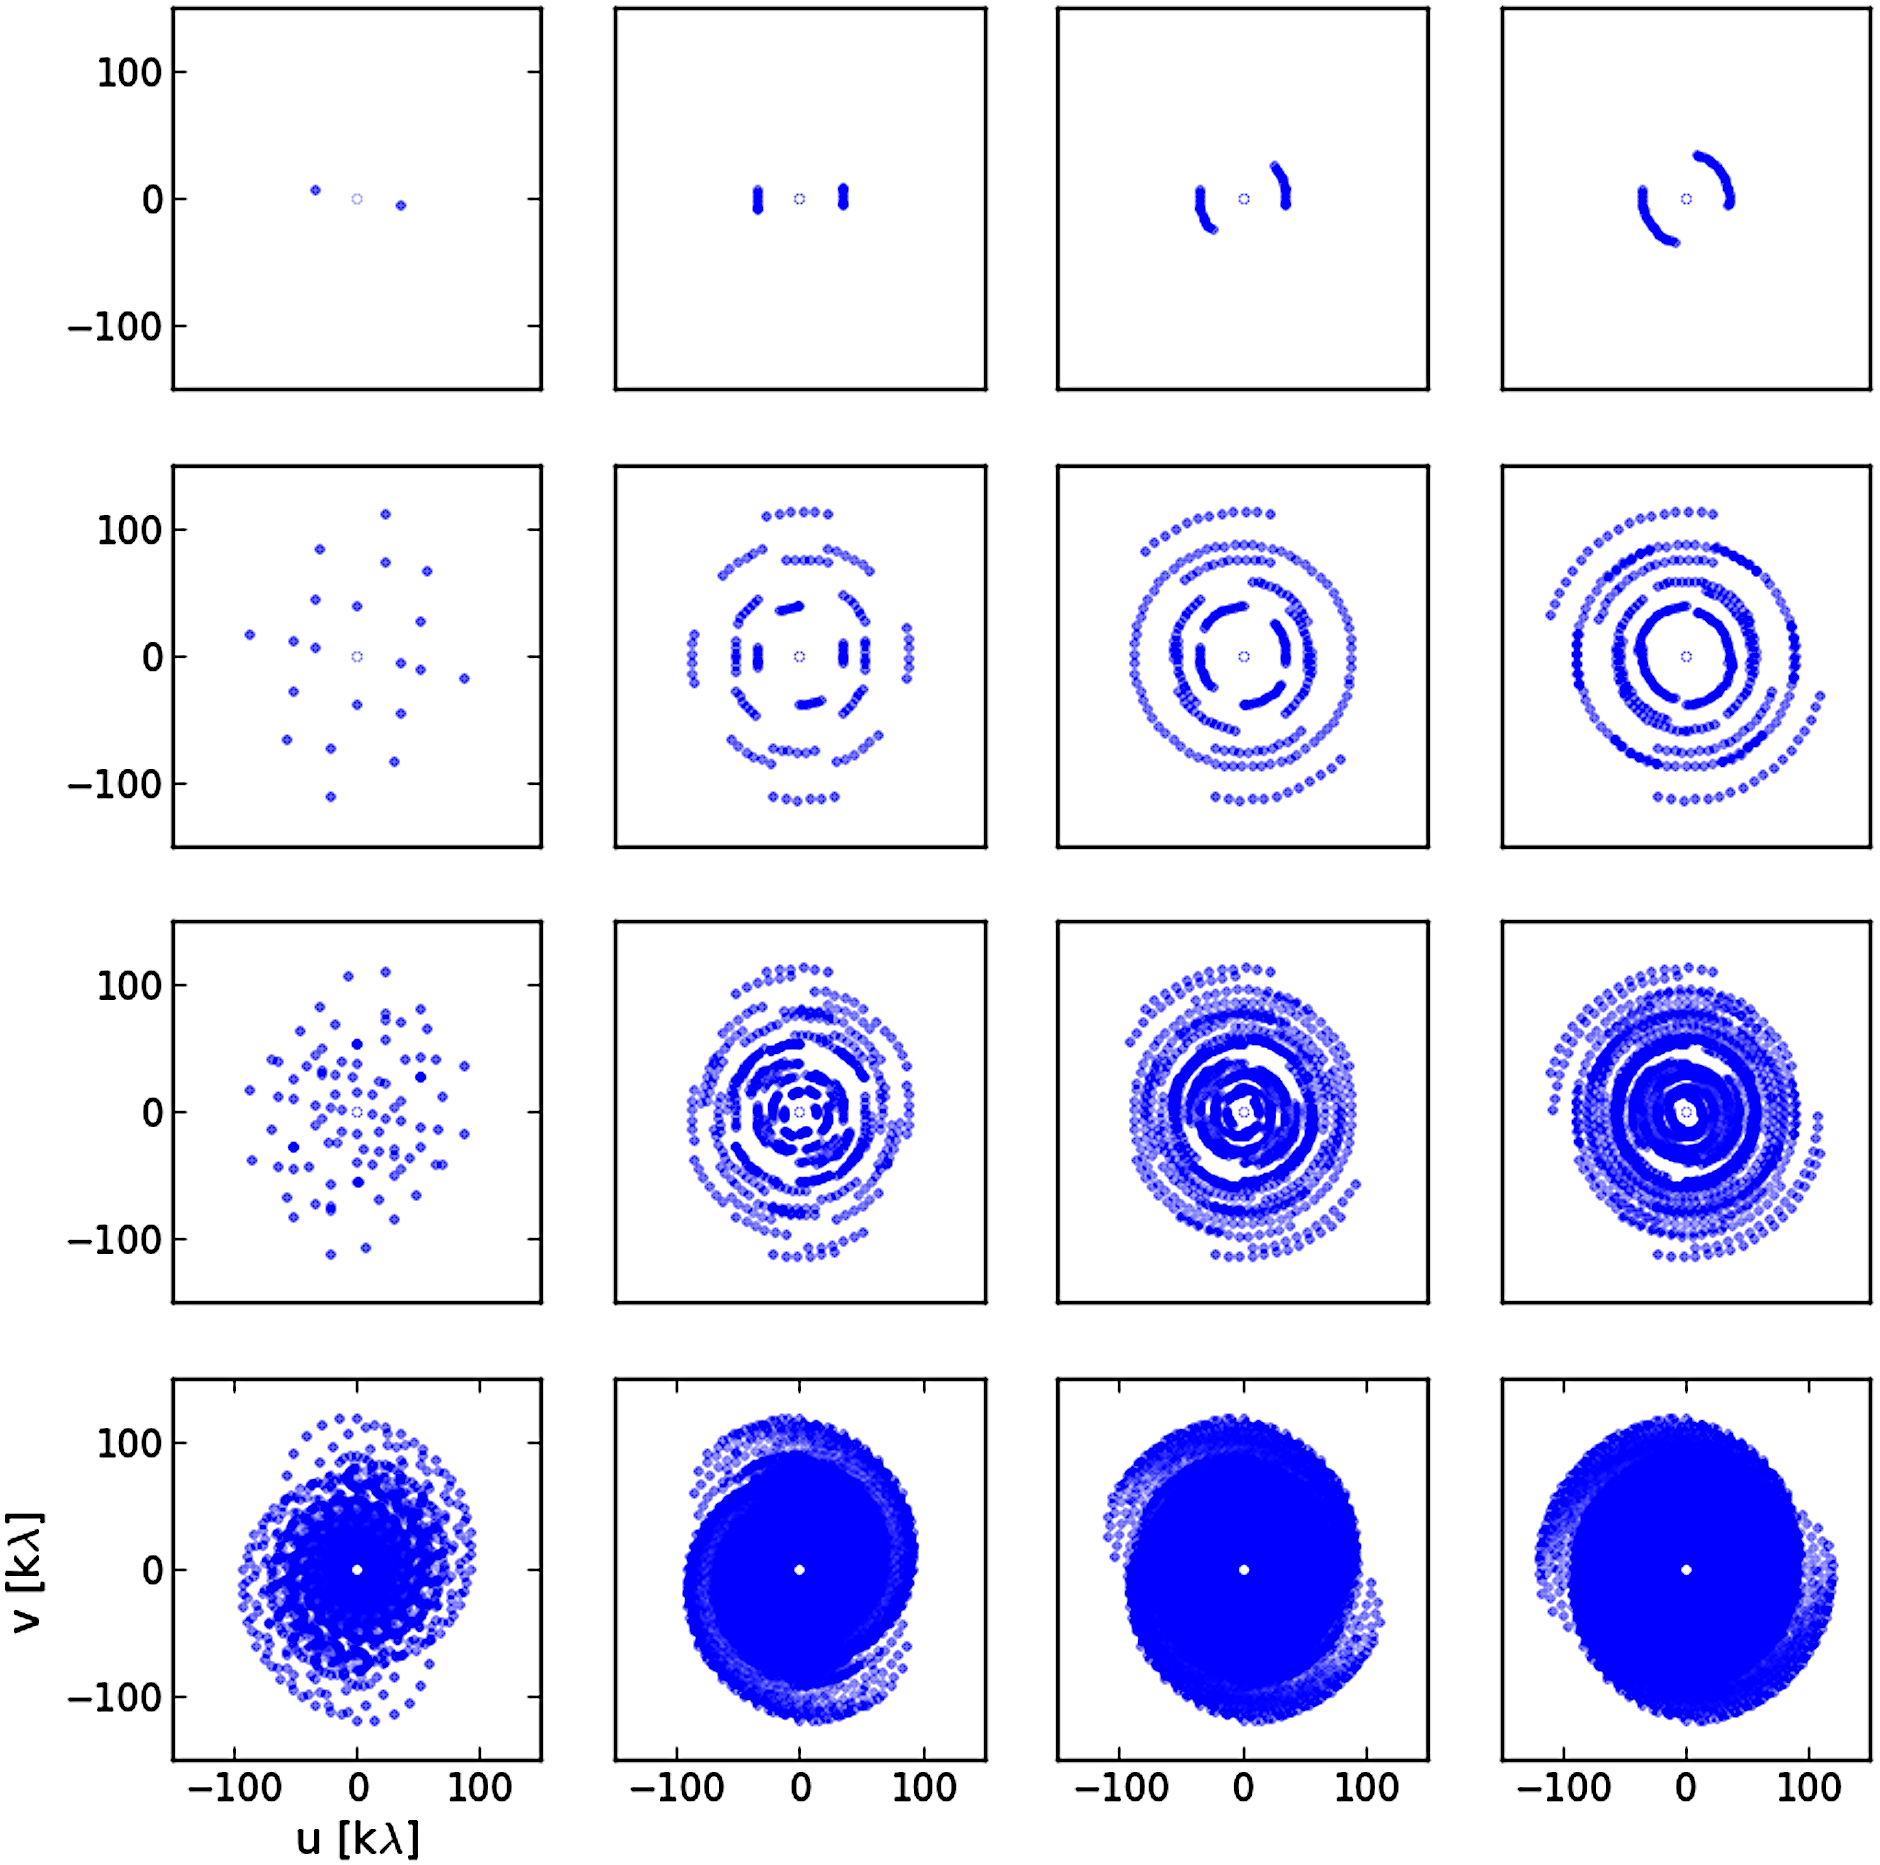
\includegraphics[width=\textwidth]{uv-coverages}
  \bicaption[$uv$ 覆盖样例]{%
    $uv$ 覆盖样例.
    \emph{从上往下:} 干涉阵列分别包括 2、5、10 和 50 个呈对数螺旋状分布的天线;
    \emph{从左到右:} 观测时间分别为 \SI{10}{\second}、\SI{2}{\hour}、
    \SI{4}{\hour} 和 \SI{6}{\hour}.
  }{%
    Examples of $uv$ coverages.
    \emph{Top to bottom:} the interferometer includes 2, 5, 10, and 50
    antennas in a logarithmic spiral pattern, respectively;
    \emph{Left to right:} the observing time is \SI{10}{\second},
    \SI{2}{\hour}, \SI{4}{\hour}, and \SI{6}{\hour}, respectively.
    \\\textcopyright{}
    \citeay{avison2013}.
  }
  \label{fig:uv-coverages}
\end{figure}

干涉阵列的天线数目总是有限的,在实际观测中 $uv$ 平面不可能被完全覆盖,
具体覆盖情况可由\emph{\acf{sf}}描述:
\begin{equation}
  \label{eq:sf}
  \acs{S-uv} = \sum_{k,t} \delta(u - u_{k,t}, v - v_{k,t}),
\end{equation}
其中 $u_{k,t}, v_{k,t}$ 为基线 $\B{b}_k$ 在 $t$ 时刻在 $uv$ 平面内的分量.
于是,干涉阵列实际测量的\ac{vis}数据为 $\acs{Vis}(u,v) \acs{S-uv}$,
由于无法获得目标亮度分布的全部信息,
根据\autoref{eq:vis-inv2} 对此进行逆 Fourier 变换
仅能得到目标的\emph{\acf{dirty-map}}:
\begin{equation}
  \label{eq:dirty-map}
  \frac{I_{\nu}^D(l,m)}{\sqrt{1-l^2-m^2}} = \iint
    \acs{Vis}(u,v) \acs{S-uv} \exp [2\Cpi\Ci\, (ul+vm)] \D{l}\D{m}.
\end{equation}
利用\ac{conv-theorem},上式可表示为:
\begin{equation}
  I_{\nu}^D(l,m) = I_{\nu}(l,m) * B(l,m),
\end{equation}
其中
\begin{equation}
  \label{eq:syn-beam}
  B(l,m) = \iint \acs{S-uv} \exp [2\Cpi\Ci\, (ul+vm)] \D{l}\D{m}
\end{equation}
是\ac{sf} \acs{S-uv} 的 Fourier 变换,
称为\emph{\acf{sb}}或\emph{\acf{psf}}.
\autoref{fig:imaging-relations} 展示了成像过程中各种变换关系.
为了从\ac{dirty-map} $I_{\nu}^D$ 尽可能地恢复目标的真实图像,
则需要使用复杂的非线性\ac{deconv}方法,
比如 CLEAN 算法 \cite{hogbom1974,cornwell1999}、
\ac{mem} \cite{narayan1986}.

\begin{figure}[htp]
  \centering
  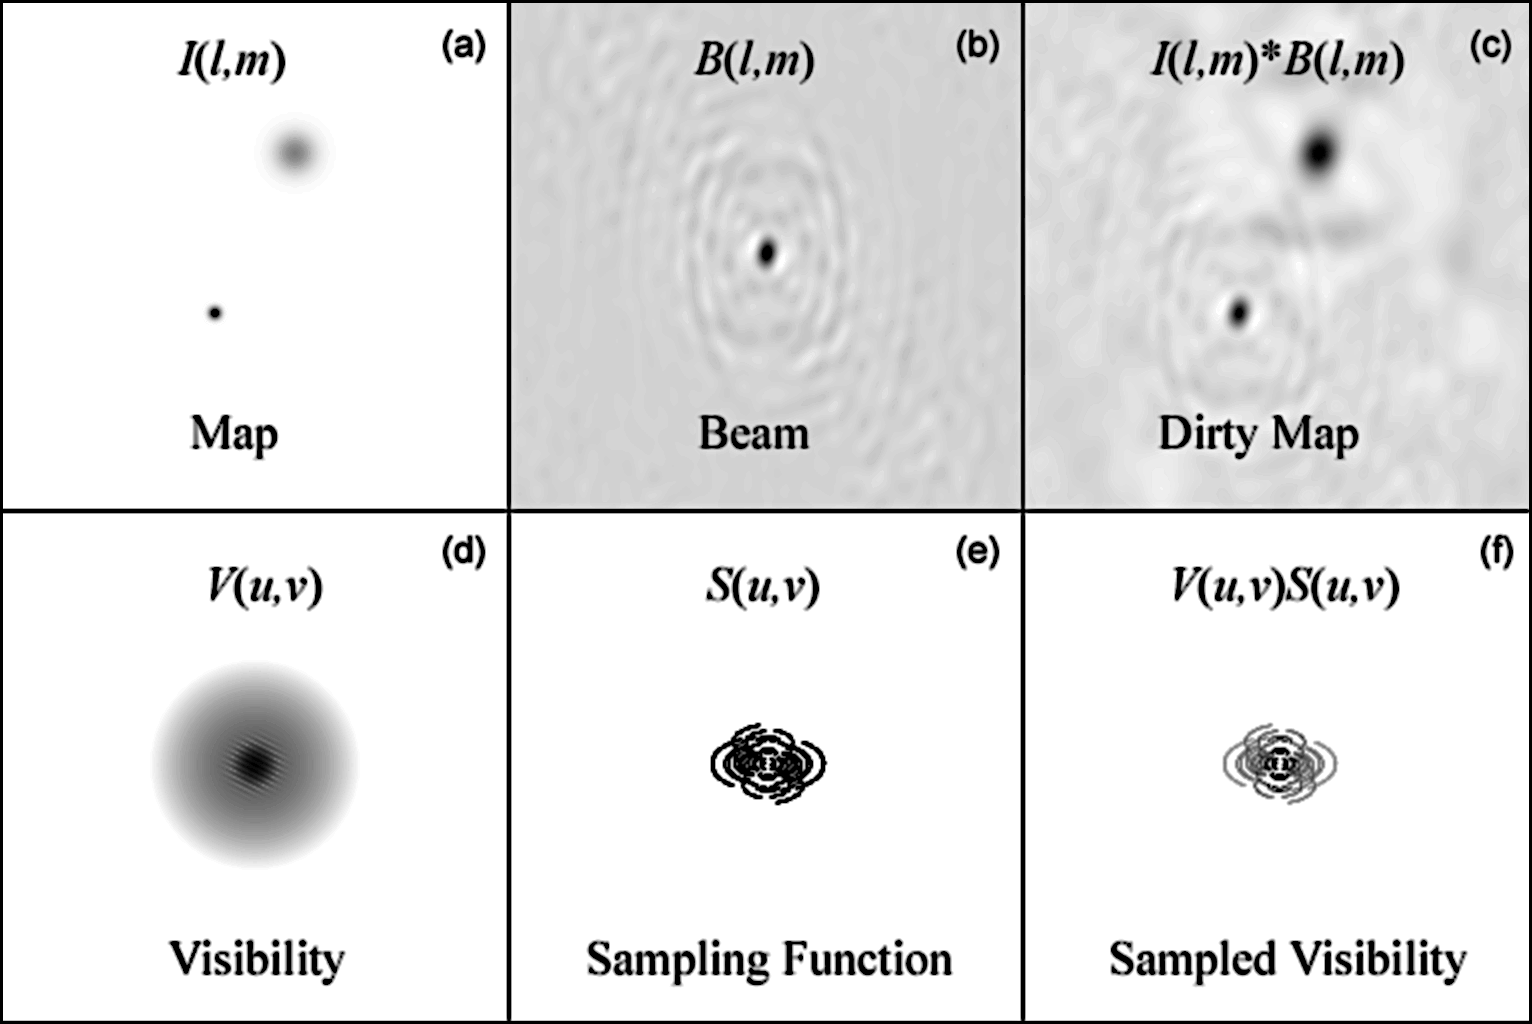
\includegraphics[width=\textwidth]{imaging-relations}
  \bicaption[成像过程中的变换关系]{%
    成像过程中的各种变换关系.
    \emph{(a)} 天空的真实图像;
    \emph{(b)} 干涉阵列的\acs*{sb},对应 (e) 的 Fourier 变换;
    \emph{(c)} 脏图,对应 (f) 的 Fourier 变换;
    \emph{(d)} \acs*{vis}的真实数据,对应 (a) 的 Fourier 变换;
    \emph{(e)} 干涉阵列的\acs*{sf};
    \emph{(f)} 实际测量到的\acs*{vis}数据,为 (d) 和 (e) 乘积.
  }{%
    The transform relations among the imaging process.
    \emph{(a)} The true sky map;
    \emph{(b)} The synthesized beam of the interferometer, which is the
    Fourier Transform of (e);
    \emph{(c)} The dirty map, which is the Fourier Transform of (f);
    \emph{(d)} The true visibility data, which are the Fourier Transform
    of (a);
    \emph{(e)} The sampling function of the interferometer;
    \emph{(f)} The actually measured visibility data, which are the
    product of (d) and (e).
    \\\textcopyright{}
    Dale E. Gary, Radio Astronomy, Lecture 6,
    \url{https://web.njit.edu/~gary/728/Lecture6.html}, (2018-11-21).
    [反转了颜色]
  }
  \label{fig:imaging-relations}
\end{figure}

%---------------------------------------------------------------------
\subsection{灵敏度}

考虑一个噪声功率的等效温度为 $T_s$ 的天线,其每个测量值的\ac{rms}误差为
$\sigma \approx \sqrt{2} T_s$
[详见 \citeay{condon2016}, 附录 B.6].
设信号的带宽为 $\Delta\nu$,根据\emph{采样定理 (sampling theorem)},
在时间 $\tau$ 内应采样 $N \gtrsim 2 \Delta\nu \,\tau$ 个数据点.
于是,对时间平均后的测量值的涨落为:
\begin{equation}
  \label{eq:radiometer}
  \sigma_T = \frac{\sqrt{2} T_s}{\sqrt{N}}
    \approx \frac{T_s}{\sqrt{\Delta\nu \,\tau}} ,
\end{equation}
其中 $\tau$ 为\ac{t-int}.
$\tau$ 越大,$\sigma_T$ 越小,则达到的灵敏度越高.
然而在实际情况中,多种系统误差会限制灵敏度的提高,
比如天线和接收机的\ac{gain}变化、大气层辐射的不规则涨落、
未分辨背景源产生的\ac{confusion}、等等。

若一个点源的辐射使天线的温度 $T_s$ 升高了 $\Delta T$,
则根据\autoref{eq:dt-source} 可测得该点源的流量密度为:
\begin{equation}
  S_{\nu} = 2\,\acs{kb} \Delta T / A_e ,
\end{equation}
相应的测量误差为:
\begin{align}
  \sigma_S
    & = \frac{2\,\acs{kb}}{A_e} \sigma(T_s + \Delta T) \\
    & \approx \frac{2\,\acs{kb}}{A_e} \sigma(T_s) \\
    & = \frac{2\,\acs{kb} T_s}{A_e \sqrt{\Delta\nu \,\tau}} .
\end{align}
此即单天线的\emph{点源灵敏度}.

对于由两个相同天线构成的二元干涉仪,其点源灵敏度为:
\begin{equation}
  \label{eq:sigma-ps1}
  \sigma_S = \frac{\sqrt{2}\,\acs{kb} T_s}{A_e \sqrt{\Delta\nu \,\tau}} .
\end{equation}
由 \acs{N-ant} 个相同天线构成的干涉仪可形成 $\acs{N-ant}(\acs{N-ant}-1)$
个独立的二元干涉仪,因此其\emph{点源灵敏度}为:
\begin{equation}
  \label{eq:sigma-ps}
  \sigma_S = \frac{2\,\acs{kb} T_s}{
    A_e \sqrt{\acs{N-ant}(\acs{N-ant}-1) \Delta\nu \,\tau}} .
\end{equation}

如果观测一个\acf{extsrc},则需要考虑干涉仪的\emph{亮度灵敏度},
可利用 Rayleigh--Jeans 近似 [\autoref{eq:rj-approx}]
直接由 $\sigma_S$ 导出:
\begin{equation}
  \label{eq:sigma-tb}
  \sigma_b = \frac{\lambda^2}{2\,\acs{kb}} \frac{\sigma_S}{\Omega_A} ,
\end{equation}
其中 $\Omega_A$ 是波束的立体角.
相比单口径望远镜,干涉仪的基线长、角分辨率高,
因此\ac{sb}的立体角 $\Omega_A$ 非常小,
从而导致其亮度灵敏度 $\sigma_b$ 明显差于单口径望远镜.


%=====================================================================
\section{主要低频干涉阵列}
\label{sec:instruments}

大型低频干涉阵列是目前测量 EoR 信号的主要设备.
近十几年以来,国内外已建成一批各具特色的低频干涉阵列,
还有若干新型干涉阵列正在兴建或准备建设.
以下对其中主要的干涉阵列作简要介绍.

%---------------------------------------------------------------------
\subsection{21CMA}

\acf{21cma} 是我国开展“宇宙第一缕曙光”探测的低频射电干涉阵列,
位于中国西部天山深处的乌拉斯台,环绕在四周的高山能提供宁静的射电环境.
\acs{21cma} 的 81 个站点呈 T 形分布在东西约 \SI{6}{\km}、
南北约 \SI{4}{\km} 的两条直线上.
\autoref{fig:21cma} 展示了沿东西方向的部分站点.
每个站点包含 127 根对数周期天线,工作频率为 \SIrange{50}{200}{\MHz},
频率分辨率为 \SI{24.4}{\kHz},
角分辨率达 \SI{1}{\arcminute}(在 \SI{200}{\MHz} 处),
采用模拟波束合成固定观测以北天极为中心、半径约 \SI{5}{\degree} 的天区
\cite{wang2013,zheng2016}.
\acs{21cma} 已于 2006 年建设完成,并于 2009 年升级了新型低噪声放大器和
基于 \acs{gpu} 的数据采集系统,目前已积累多年的观测数据.
\acs{21cma} 作为中国主要的 \acs{ska} 探路者项目,
项目成员开发了完整的数据处理流程及软件、
提出了射频干涉探测及抑制新方法 \cite{huang2016}、
探测并编录了北天极视场内的 624 个射电源 \cite{zheng2016}.
目前,\acs{21cma} 正在改造升级数字多波束合成系统,
以实现多目标跟踪观测,掌握低频脉冲星的搜寻技术.

\begin{figure}[htp]
  \centering
  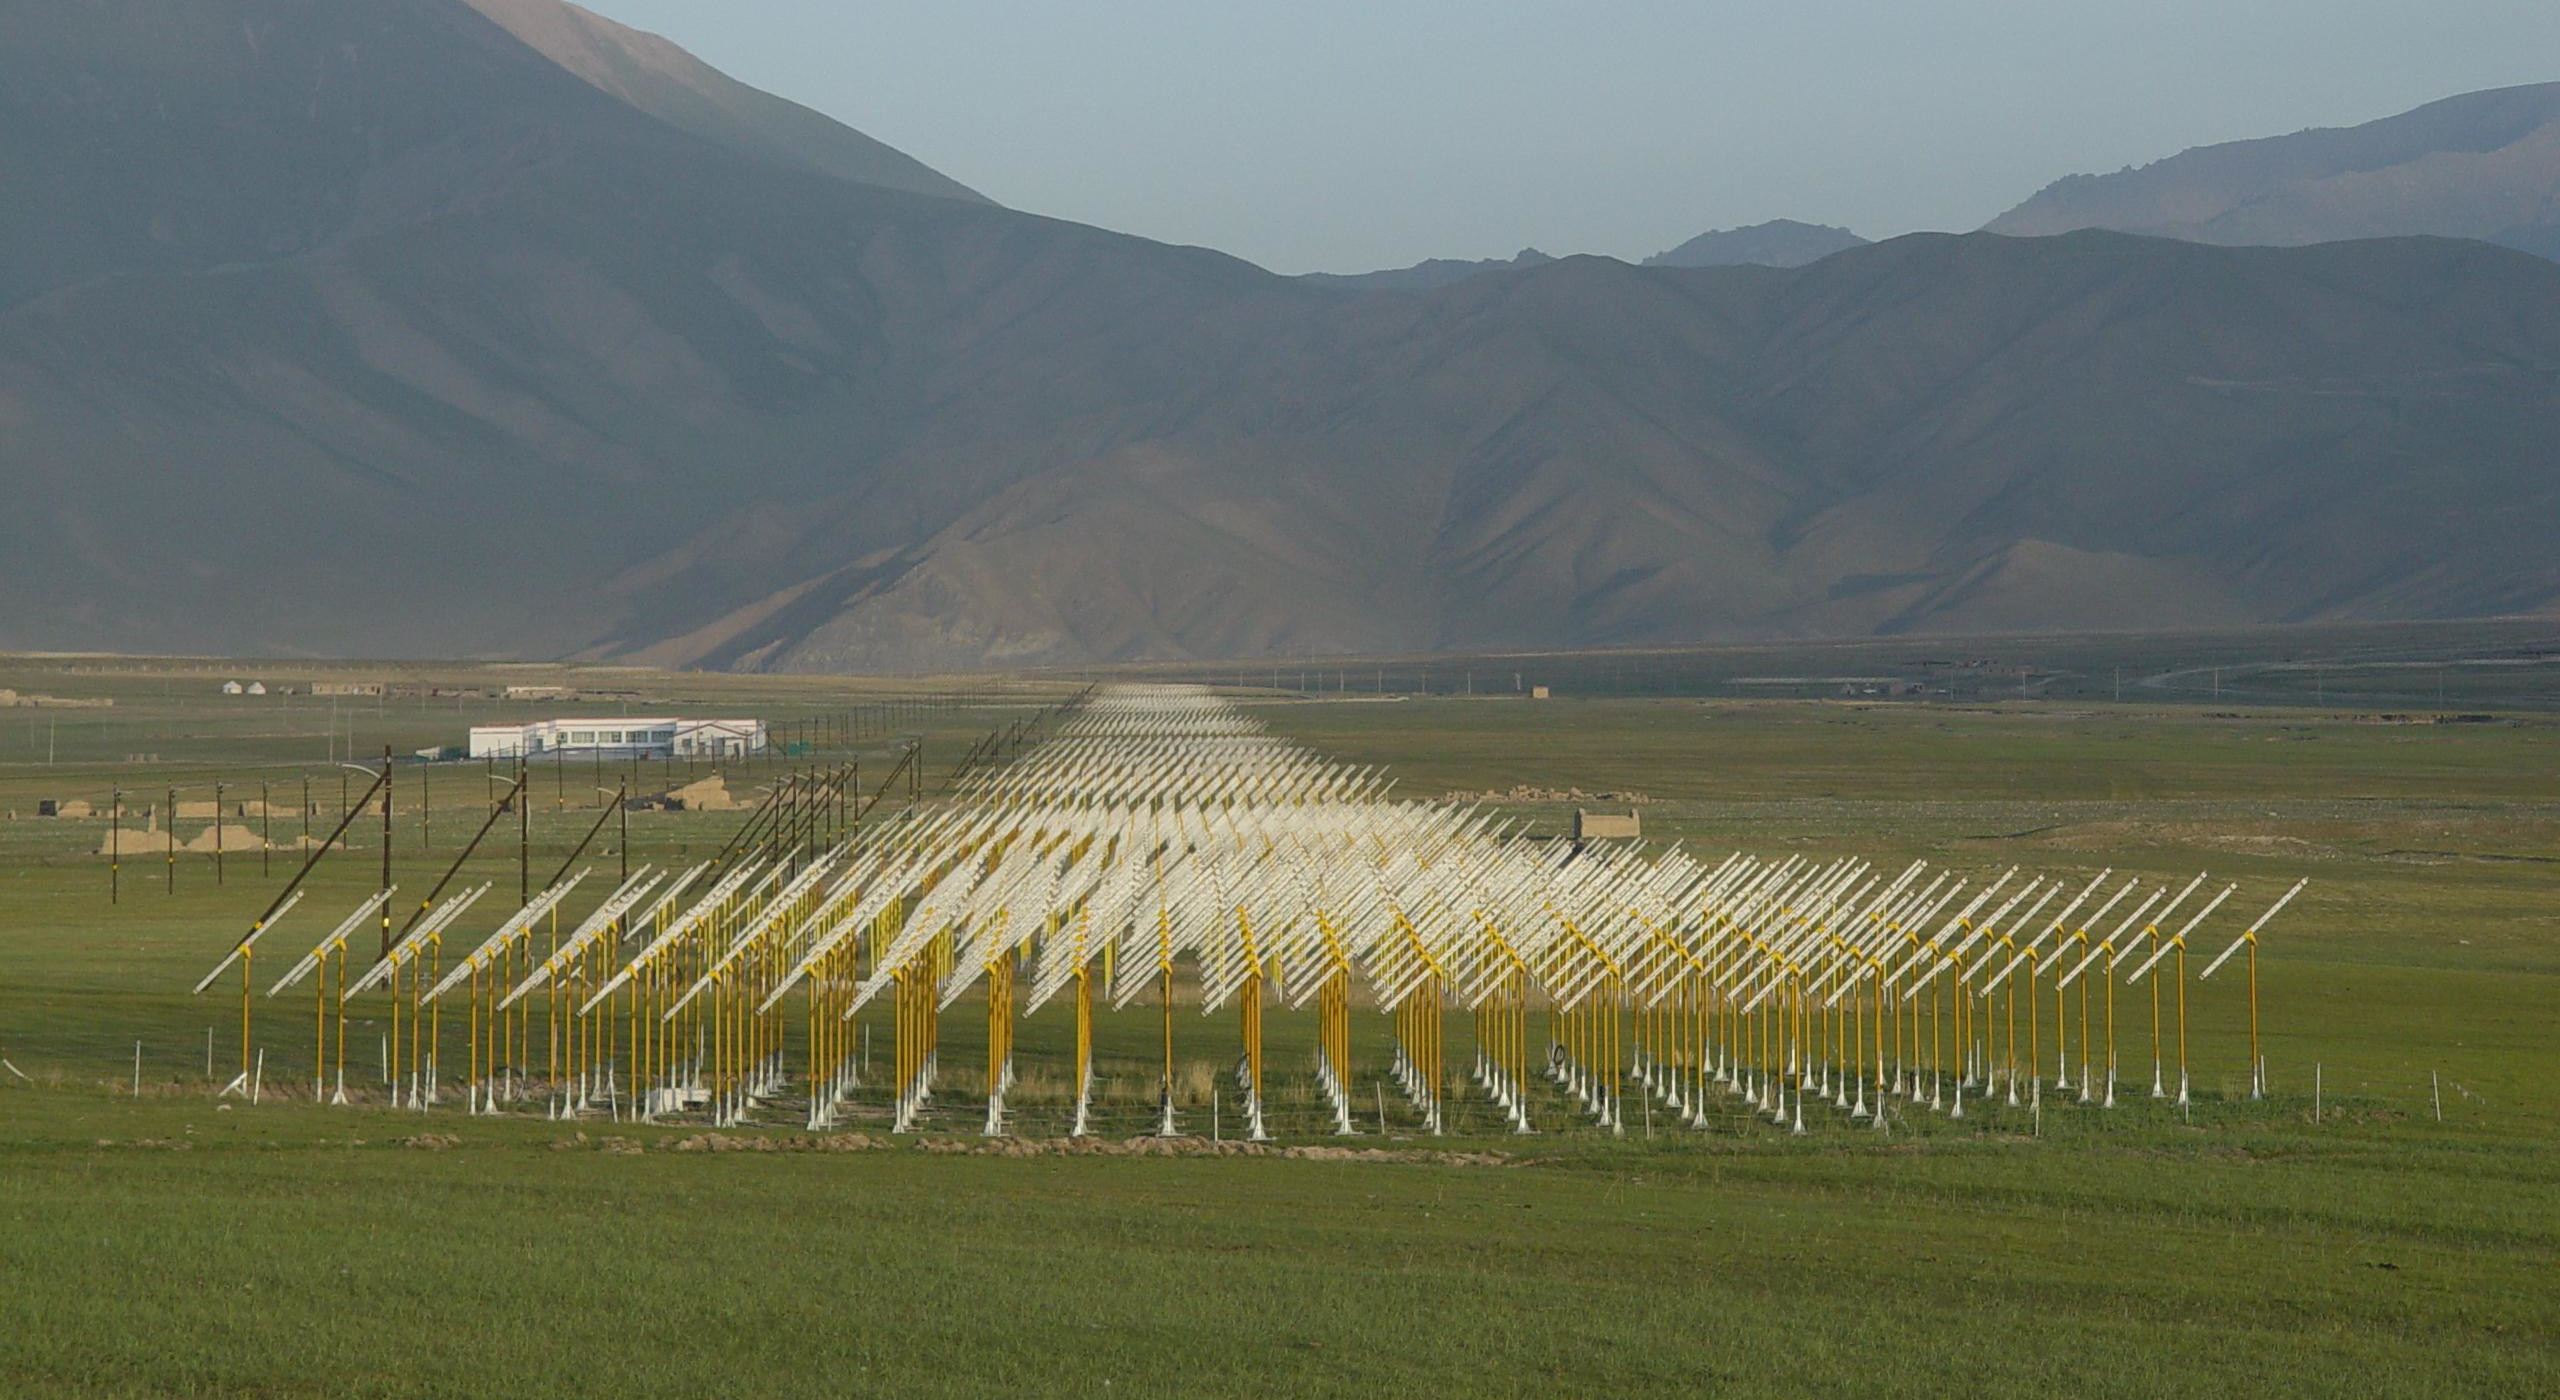
\includegraphics[width=0.8\textwidth]{21CMA}
  \bicaption[21CMA 东西方向的部分站点]{%
    21CMA 东西方向的部分站点,每个站点包含 127 根对数周期天线.
  }{%
    Part of the 21CMA stations along the east-west direction,
    with each station including 127 log-periodic antennas.
    \\\textcopyright{}
    21CMA, \acuse{nao}\acl{nao}.
  }
  \label{fig:21cma}
\end{figure}

%---------------------------------------------------------------------
\subsection{LOFAR}

\acf{lofar} 是由 \ac{astron} 建造的新型低频干涉阵列 \cite{vanHaarlem2013},
由工作在 \SIrange{10}{90}{\MHz} 波段的低频段天线(LBA)和
工作在 \SIrange{110}{250}{\MHz} 波段的高频段天线(HBA)两部分组成.
\acs{lofar} 共有 51 个站点,
其中 24 个站点分布在半径 \SI{2}{\km} 的核心区域
(\autoref{fig:lofar} 显示了最中心的部分),
14 个站点呈螺旋状分布在外围区域,
还有 13 个国际站点分布在德国、法国、瑞士、英国、波兰和爱尔兰,
基线长达 \SI{1500}{\km}.
荷兰境内的 38 个站点各包含 96 个 LBA 和 48 个 HBA,
13 个国际站点每个包含 96 个 LBA 和 96 个 HBA.
\acs{lofar} 采用了数字多波束合成技术,能实现多目标跟踪观测,
并且显著提高巡天效率,为 SKA1-Low 提供强有力的技术支持
\cite{deVos2009,vanHaarlem2013,pizzo2018}.
\acs{lofar} 于 2012 年建设完成并开始观测,
已经完成北天 \SIrange{120}{168}{\MHz} 的深度巡天
\ac{lotss} \cite{shimwell2017,shimwell2019}.
目前,\acs{lofar} 正在提议 2.0 升级计划.

\begin{figure}[htp]
  \centering
  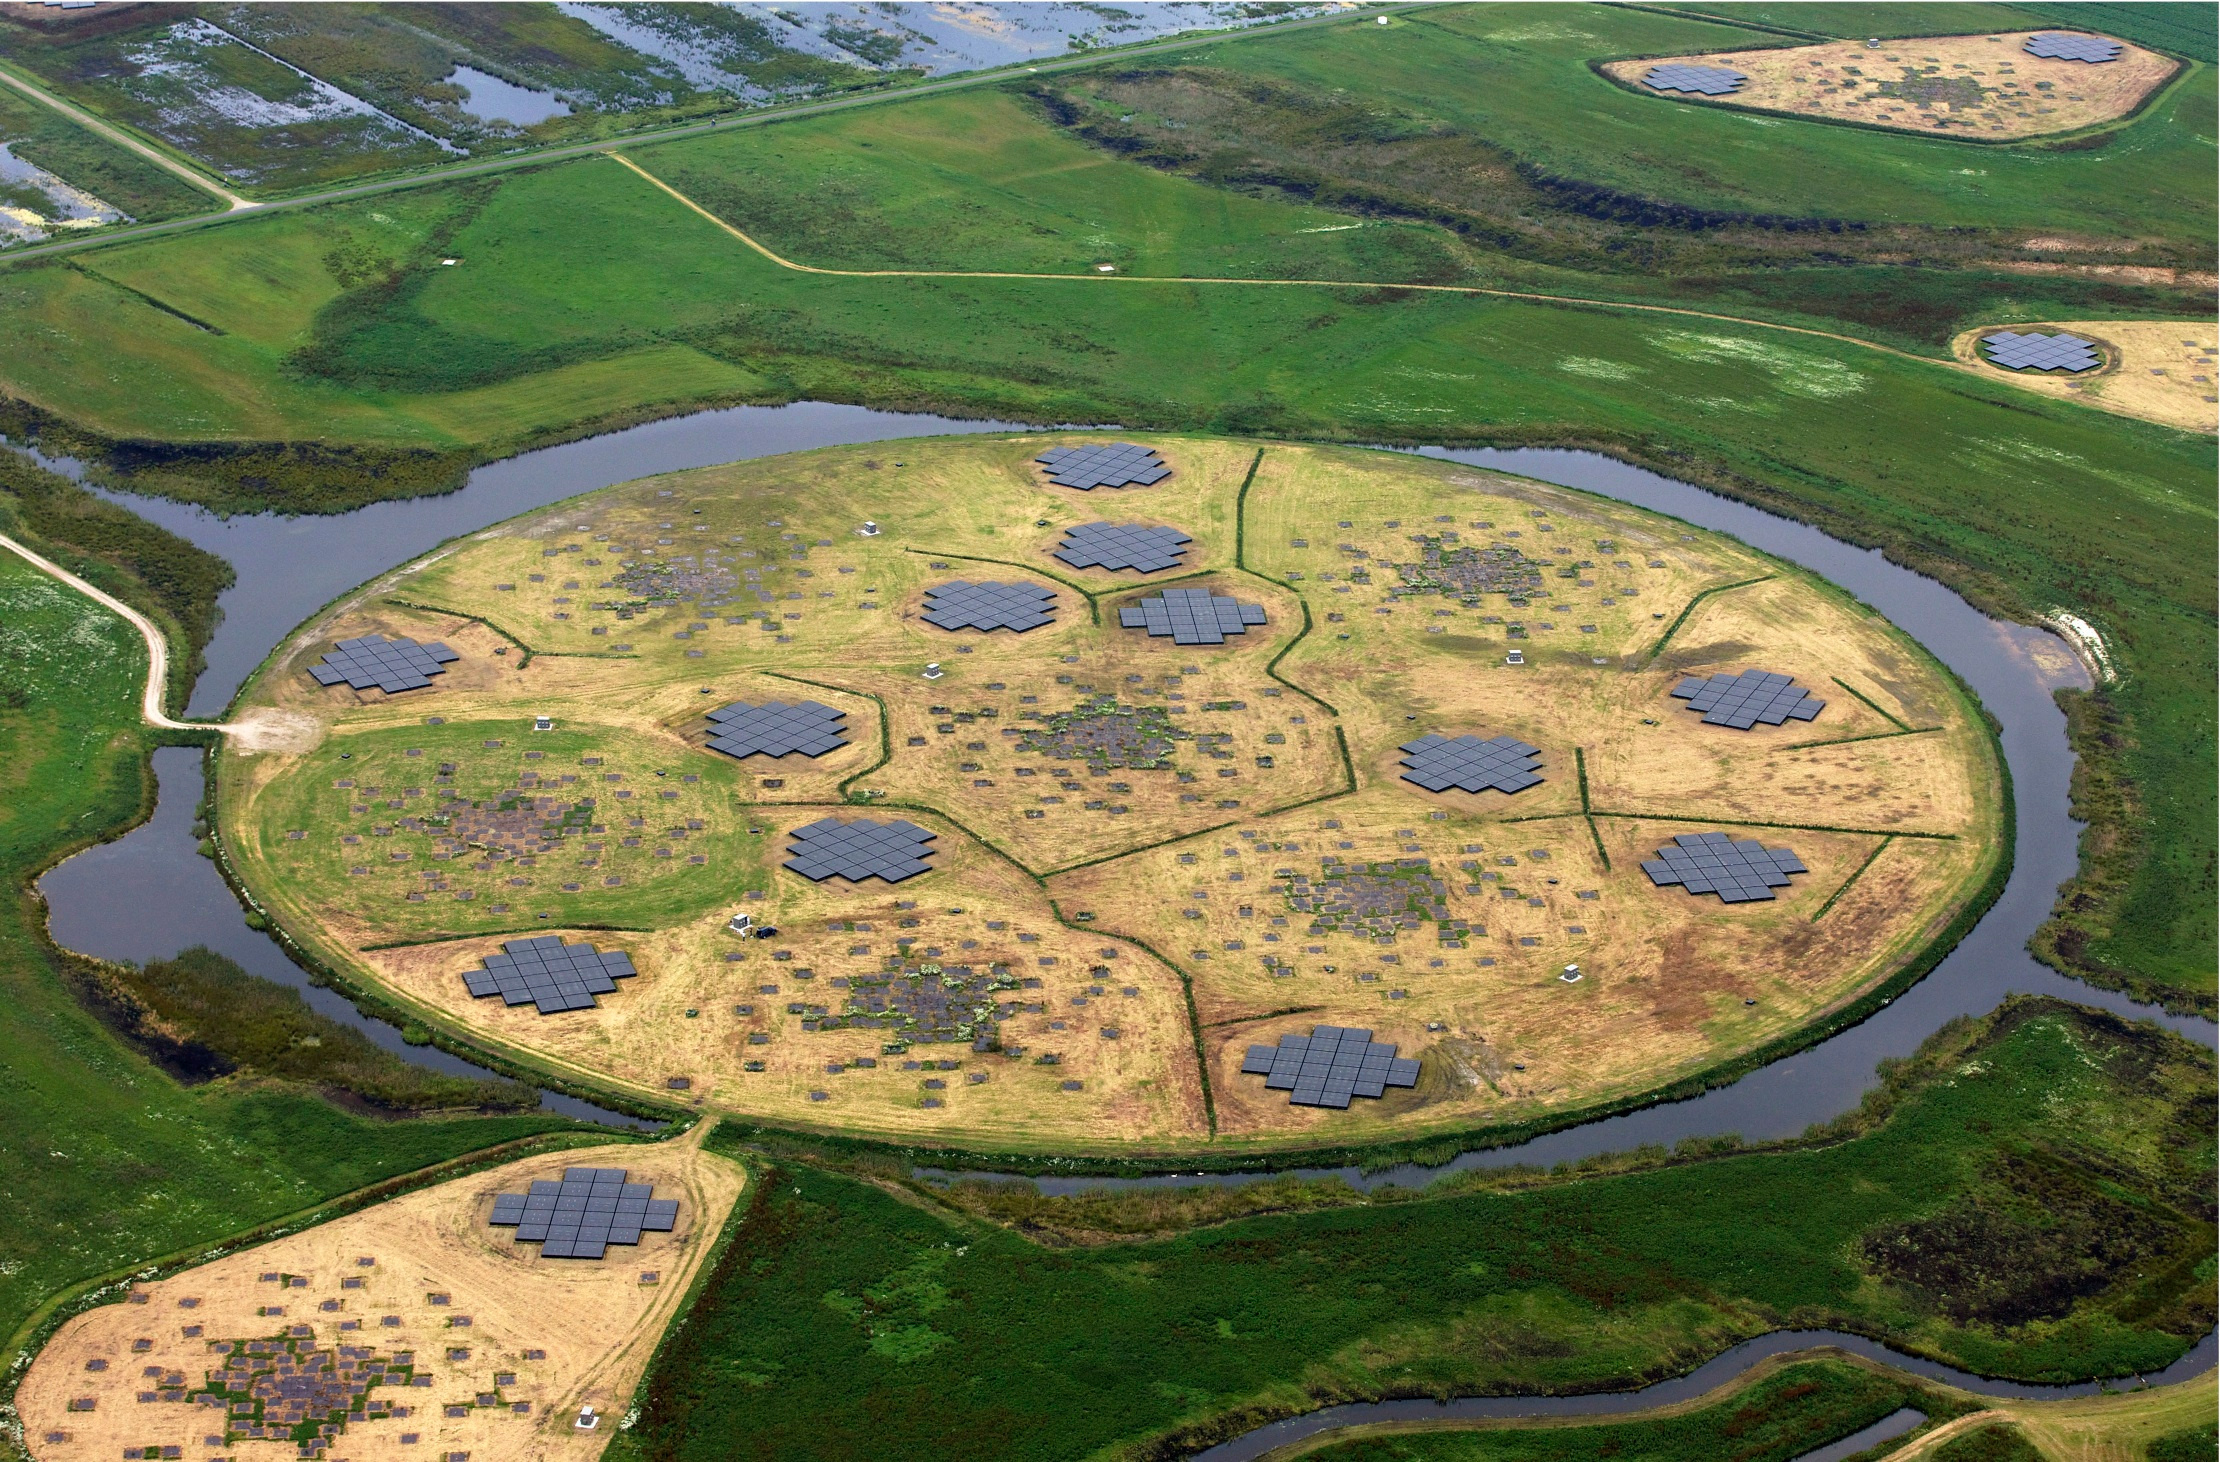
\includegraphics[width=0.8\textwidth]{LOFAR-superterp}
  \bicaption[LOFAR 核心区域的中心]{%
    \acs{lofar} 核心区域的中心.
    小块深色区域为 LBA,大块深色区域为 HBA.
  }{%
    The heart of the \acs{lofar} core.
    The small dark regions are installed with LBA,
    while the big dark regions are installed with HBA.
    \\\textcopyright{}
    \citeay{vanHaarlem2013}.
  }
  \label{fig:lofar}
\end{figure}

%---------------------------------------------------------------------
\subsection{MWA}

\acf{mwa} 位于澳大利亚西部的 Murchison 射电天文台,是 SKA1-Low 的先驱
\cite{lonsdale2009,bowman2013,tingay2013,wayth2018}.
该阵列的主要科学目标包括宇宙再电离信号探测、河内及河外射电源、暂现源和空间气候.
\acs{mwa} 工作在 \SIrange{80}{300}{\MHz} 频段,使用一种双极化偶极子天线,
每个站点包含 16 个天线(按 4 行 4 列规则排列).
所有天线均固定指向天顶,工作时通过调控各天线的时延来控制波束的合成与指向.
\acs{mwa} 自 2007 年开始建设,于 2012 年完成了一期 128 个站点的建设,
于 2017 年底完成了二期 128 个新站点的扩建工作\cite{wayth2018},目前已投入使用.
\autoref{fig:mwa} 显示了 \acs{mwa} 东侧六边形区域内的站点.
\acs{mwa} 的站点分为两部分:
一部分紧凑地排列在六边形区域内,主要用于探测再电离信号以及研究银河系大尺度结构;
另一部分散布于四周较大区域,实现较高的空间分辨率,便于开展河外射电源等研究.
\acs{mwa} 一期已完成了 \ac{gleam} 巡天项目 \cite{wayth2015},
并已发布一批成果,比如点源目录 \cite{hurleyWalker2017}、
银河系内 \Hii/ 区目录 \cite{su2018}、
高分辨率 EoR 前景模型 \cite{procopio2017}、等等.
使用 \acs{mwa} 二期开展的 \ac{gleam-x} 巡天也正在积极进行 \cite{hurleyWalker2017prop}.
作为少有的覆盖南天的低频射电巡天,\acs{gleam} 和 \acs{gleam-x}
将为 SKA1-Low 的巡天工作提供校准指导和星表的交叉认证.
同时 \acs{mwa} 也将会为 SKA1-Low 的宇宙再电离探测任务提供
更精准的天空模型和天区指导.

\begin{figure}[htp]
  \centering
  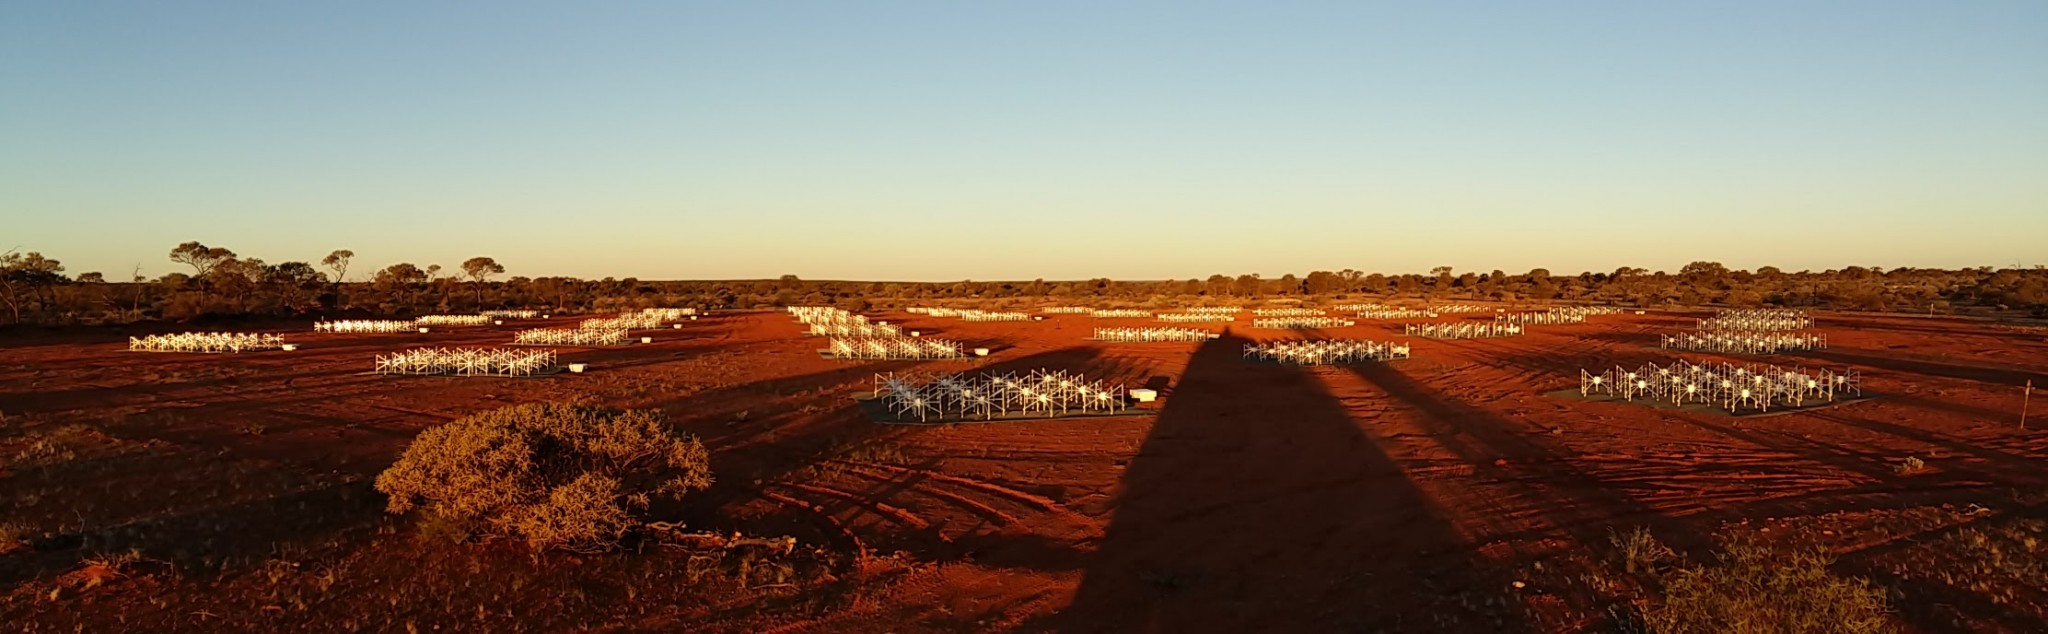
\includegraphics[width=\textwidth]{MWA}
  \bicaption[MWA 东部站点]{%
    \acs{mwa} 东侧六边形区域内的站点,每个站点包含 16 个天线.
  }{%
    The stations inside the \acs{mwa}'s east hexagonal region,
    with each station consisting of 16 antennas.
    \\\textcopyright{}
    \acuse{icrar}\ac{icrar}/\acs{mwa},
    \url{https://www.icrar.org/multimedia/images/}, (2018-10-04).
  }
  \label{fig:mwa}
\end{figure}

%---------------------------------------------------------------------
\subsection{LWA}

\acf{lwa} 是一个正在建设于美国新墨西哥州中部的大型低频干涉阵列,
计划由 53 个分布远达 \SI{400}{\km} 的站点组成,
每个站点的大小约 \SI{100x100}{\meter} 并且包含 256 个双极化天线,
总接收面积达 \SI{1}{\km\squared}(在 \SI{10}{\MHz} 处),
工作在非常低频的 \SIrange{10}{88}{\MHz} 波段,
这是我们目前了解最少的射电波段 \cite{ellingson2009}.
借助其高灵敏度和高角分辨率,\acs{lwa} 将打开这一个新射电窗口,
研究宇宙高能粒子加速机制、早期宇宙及其演化、暂现源、银河系星际介质、
太阳活动及电离层性质等.
\acs{lwa} 所采用的大站点设计使其更适合研究银河系的大尺度结构.
\acs{lwa} 的首个站点(LWA1;\autoref{fig:lwa})位于\ac{vla} 附近,
已于 2009 年建设完成,并于 2011 年开始正式观测 \cite{taylor2012,ellingson2013};
其他站点正在积极建设之中.
\acs{lwa} 亦采用数字波束合成技术,但其创新之处在于每个站点均可独立使用并成像.
目前已使用 \acs{lwa}1 开展巡天并获得了 \SIrange{35}{80}{\MHz}
北天图像 \cite{dowell2017}.

\begin{figure}[htp]
  \centering
  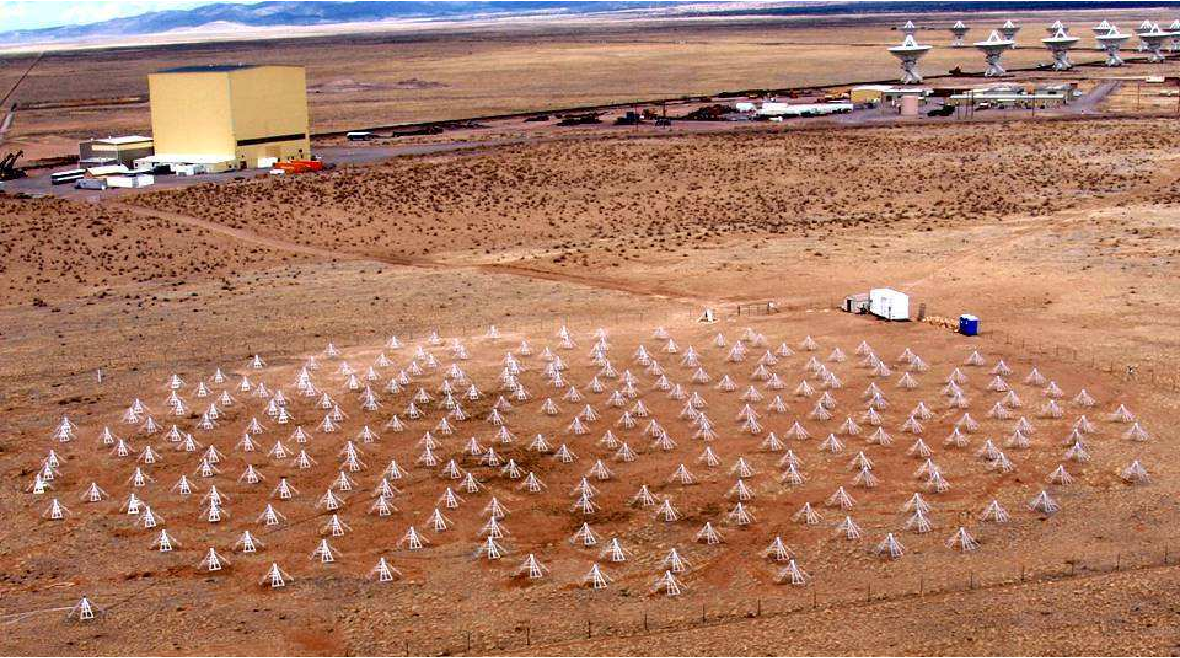
\includegraphics[width=0.8\textwidth]{LWA1}
  \bicaption[LWA 的首个站点(LWA1)]{%
    位于 \acs{vla} 附近的 \acs{lwa} 的首个站点(LWA1),包含 256 个天线.
  }{%
    The first station of \acs{lwa}, i.e., LWA1,
    which locates near the \acs{vla} and contains 256 antennas.
    \\\textcopyright{}
    \citeay{taylor2012}.
  }
  \label{fig:lwa}
\end{figure}

%---------------------------------------------------------------------
\subsection{MITEoR}
\label{ssec:miteor}

\acf{miteor} 是一个使用\ac{fftt} 新技术\cite{tegmark2009,tegmark2010}的先导阵列,
由 64 个按 8 行 8 列规则分布的全同双极化天线构成(\autoref{fig:miteor}),
在 \SIrange{100}{200}{\MHz} 范围内覆盖两个宽度为 \SI{25}{\MHz} 的频段
\cite{zheng2014}.
利用这种天线布局方式,可以直接对天线采集信号运用\ac{fft}进行成像,
避免了传统干涉阵列耗时的天线/站点间两两相关运算,
将计算复杂度由 $O(N_{\!A}^2)$ 显著降为 $O(\acs{N-ant} \log\acs{N-ant})$,
其中 \acs{N-ant} 为\acl{N-ant};
同时还将数据存储压力从 $O(N_{\!A}^2)$ 大幅减轻至 $O(\acs{N-ant})$.
如此可以极大地降低建设和运行成本,非常有利于建设超大规模的干涉阵列,
实现极高的灵敏度.
此外,阵列中的大量冗余基线能为系统自校准提供有效帮助 \cite{dillon2016}.
目前,\ac{miteor} 已开展观测并公布了 \SIrange{128}{175}{\MHz} 的北天图像
\cite{zheng2017},充分验证了 \ac{fftt} 技术的可行性.
该技术的创新性和巨大潜力能在未来 EoR 实验中发挥重要作用.

\begin{figure}[htp]
  \centering
  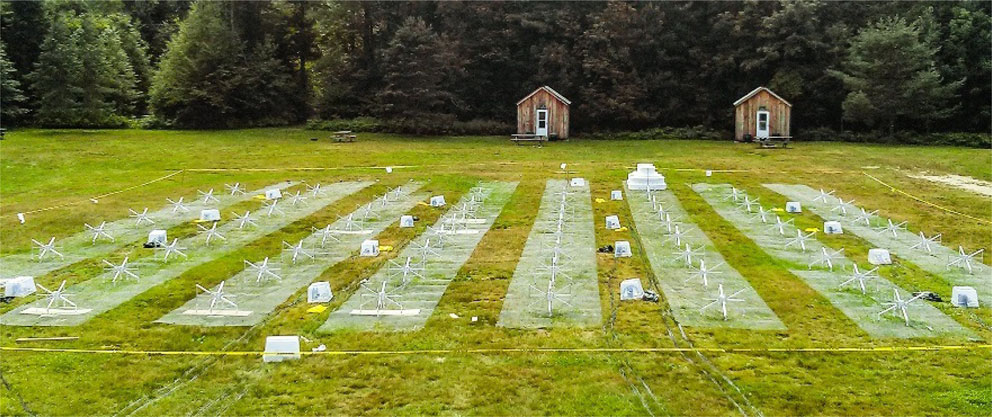
\includegraphics[width=\textwidth]{MITEoR}
  \bicaption[MITEoR 干涉阵列]{%
    在 2013 年夏天部署完成的 \acs{miteor} 干涉阵列,
    64 个双极化天线规则地分布在 \SI{21x21}{\meter} 的矩形区域,
    相互之间分隔 \SI{3}{\meter}.
  }{%
    The \acs{miteor} array deployed in the summer of 2013.
    The 64 dual-polarization antennas were laid on a \SI{21x21}{\meter}
    regular grid with a separation of \SI{3}{\meter}.
    \\\textcopyright{}
    \citeay{zheng2014}.
  }
  \label{fig:miteor}
\end{figure}

%---------------------------------------------------------------------
\subsection{HERA}

\acf{hera} 是正在南非 Karoo 射电天文保护区建造的、
继 \ac{paper} 等探路者阵列之后的第二代宇宙再电离时期探测阵列 \cite{deboer2017}.
其首要科学目标是精确测量源自宇宙再电离时期甚至\ac{cd}时期的 21\,cm 信号
及其功率谱的演化,从而描绘宇宙再电离时期以及之前的宇宙大尺度结构.
该阵列将由 350 面直径为 \SI{14}{\meter} 的固定式抛物面碟形天线构成,
观测频率为 \SIrange{50}{250}{\MHz}.
\acs{hera} 的阵型和天线设计保证了它能够为 EoR 信号的观测提供高灵敏度、
波束形状和其他仪器效应相对简单可控、
易于借助大量冗余基线对系统进行高精度校准 \cite{dillon2016}.
该设计还保证 \acs{hera} 能够有效利用\ac{delay-spec} 技术\cite{parsons2012}
和\ac{fgavd}方法(详见 \autoref{sec:fgavd})来处理观测数据.
目前 \acs{hera} 的第一期 37 面天线已经安装完毕并开始试观测
(\autoref{fig:hera} 显示了 \acs{hera} 已于 2016 年建成的 19 面天线),
第二期的 128 面天线也已开始建设,是 SKA1-Low 的有力竞争者.

\begin{figure}[htp]
  \centering
  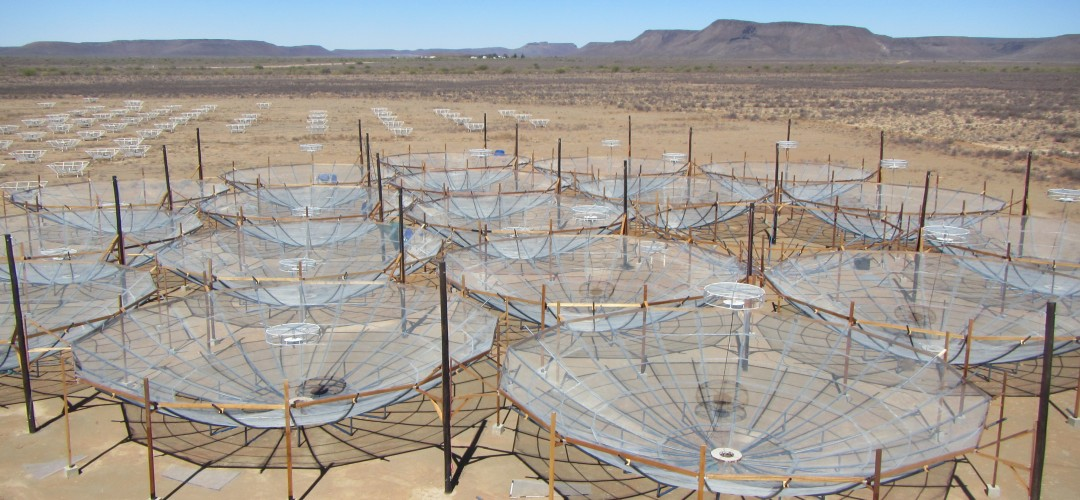
\includegraphics[width=\textwidth]{HERA19}
  \bicaption[HERA 已建成的 19 面天线]{%
    \acs{hera} 在 2016 年建成的 19 面碟形天线.
    后方的小型天线属于 \acs{paper} 项目.
  }{%
    The \acs{hera}'s 19 dish antennas deployed in South Africa in 2016.
    The small antennas in the background belong to the \acs{paper}
    experiment.
    \\\textcopyright{}
    \acs{hera}/SKA Africa, \url{http://reionization.org/}, (2018-10-04).
  }
  \label{fig:hera}
\end{figure}

%---------------------------------------------------------------------
\subsection{SKA}

\acf{ska} 是由澳大利亚、加拿大、中国、印度、意大利、新西兰、南非、瑞典、荷兰
以及英国共同参与建设的下一代巨型射电望远镜阵列,
由位于澳大利亚西部 Muchison 的低频阵列 (SKA-Low)
和位于南非 Karoo 的中频阵列 (SKA-Mid) 组成(\autoref{fig:ska}),
计划最终包含上百万个低频天线和上千面中频碟形天线,
达到约 \SI{1}{\km\squared} 的接收面积,
实现极高的灵敏度、分辨率和巡天速度.
SKA 的建设分别两期,第一期 (SKA1) 将建设约 \SI{10}{\percent} 的天线.
SKA1-Low 将由分布在 512 个站点的约 13 万根天线组成,最长基线约 \SI{65}{\km},
观测频率为 \SIrange{50}{350}{\MHz};
SKA1-Mid 将由 197 面(包含 MeerKAT 的 64 面)碟形天线组成,
最长基线约 \SI{150}{\km},观测频率为 \SI{350}{\MHz} 至 \SI{15.3}{\GHz}.
SKA 的关键科学目标有\cite{braun2015}:
宇宙再电离时期和黎明时期(功率谱测量甚至直接成像观测)\cite{mellema2013,mellema2015,koopmans2015}、
宇宙学和暗能量\cite{maartens2015,santos2015}、
脉冲星和黑洞\cite{kramer2015}、
星系形成与演化(连续谱巡天和中性氢巡天)\cite{prandoni2015,staveley2015}、
暂现源\cite{fender2015}、
宇宙磁场的起源与演化\cite{johnston2015}、
以及地外生命\cite{hoare2015}.
目前 SKA1 已在积极建设之中,预计 2025 年左右能够使用部分天线开展科学观测.

\begin{figure}[htp]
  \centering
  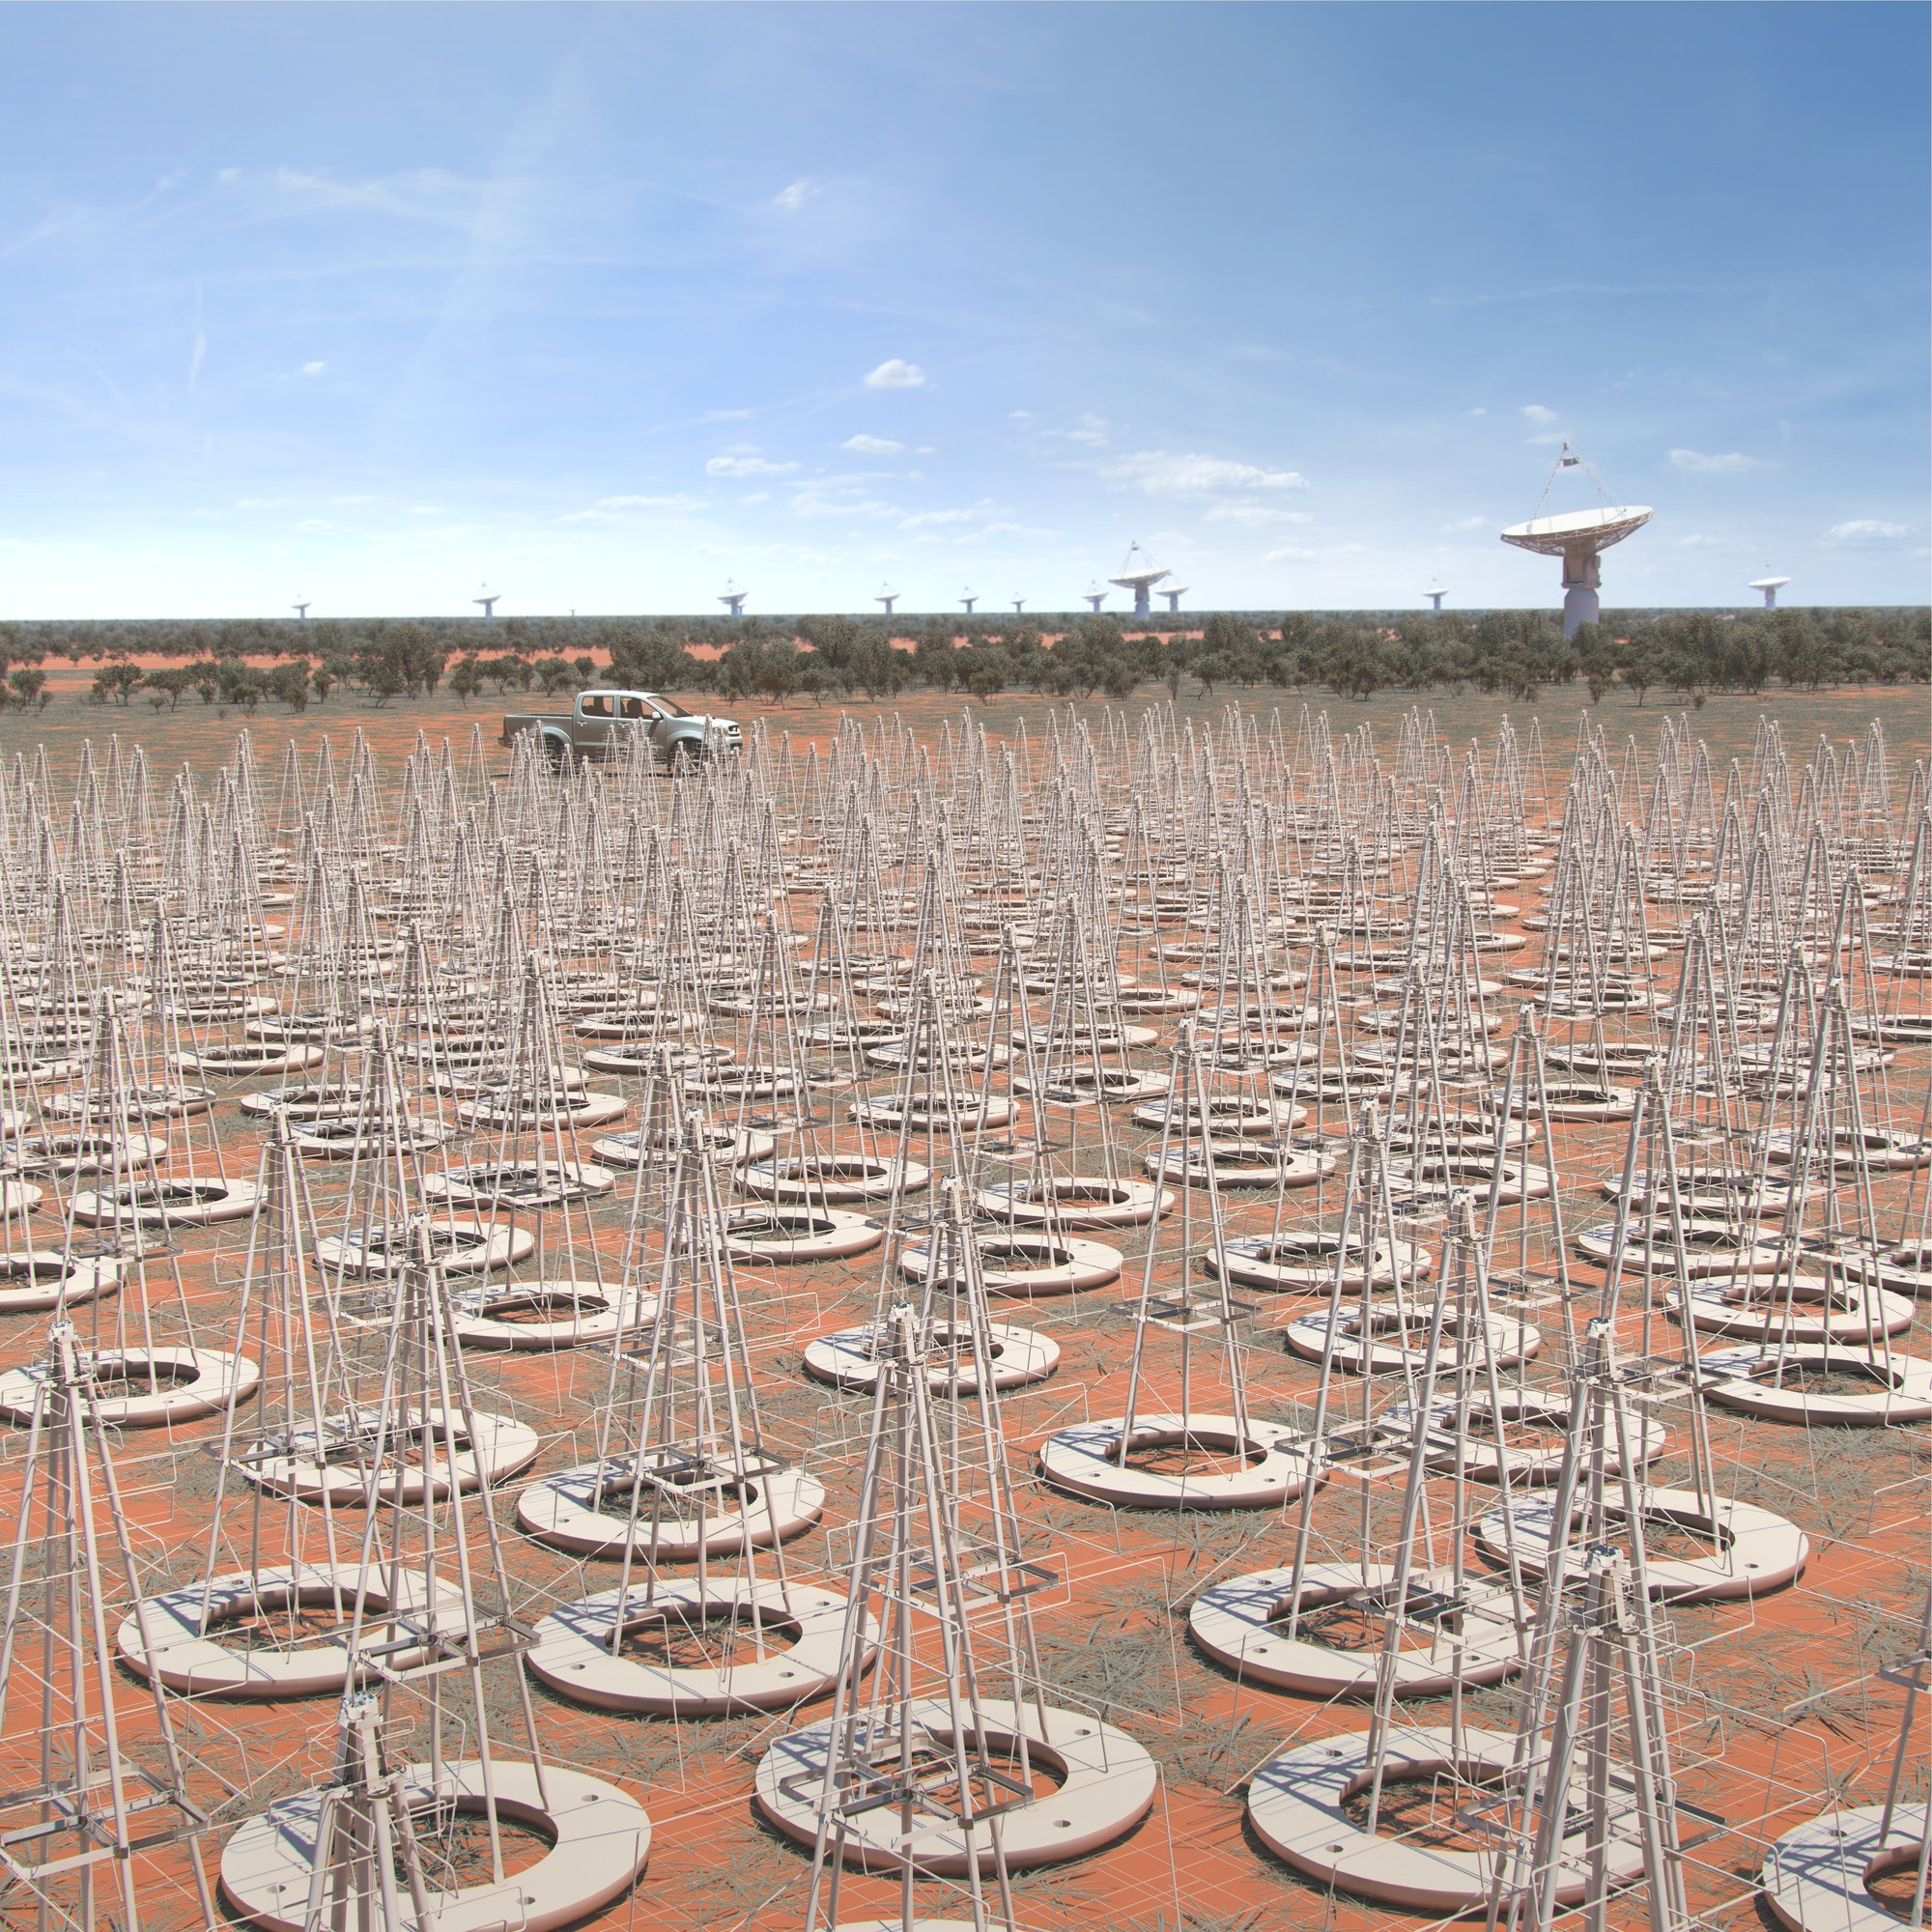
\includegraphics[width=0.5\textwidth]{SKA1-low-closeup}%
  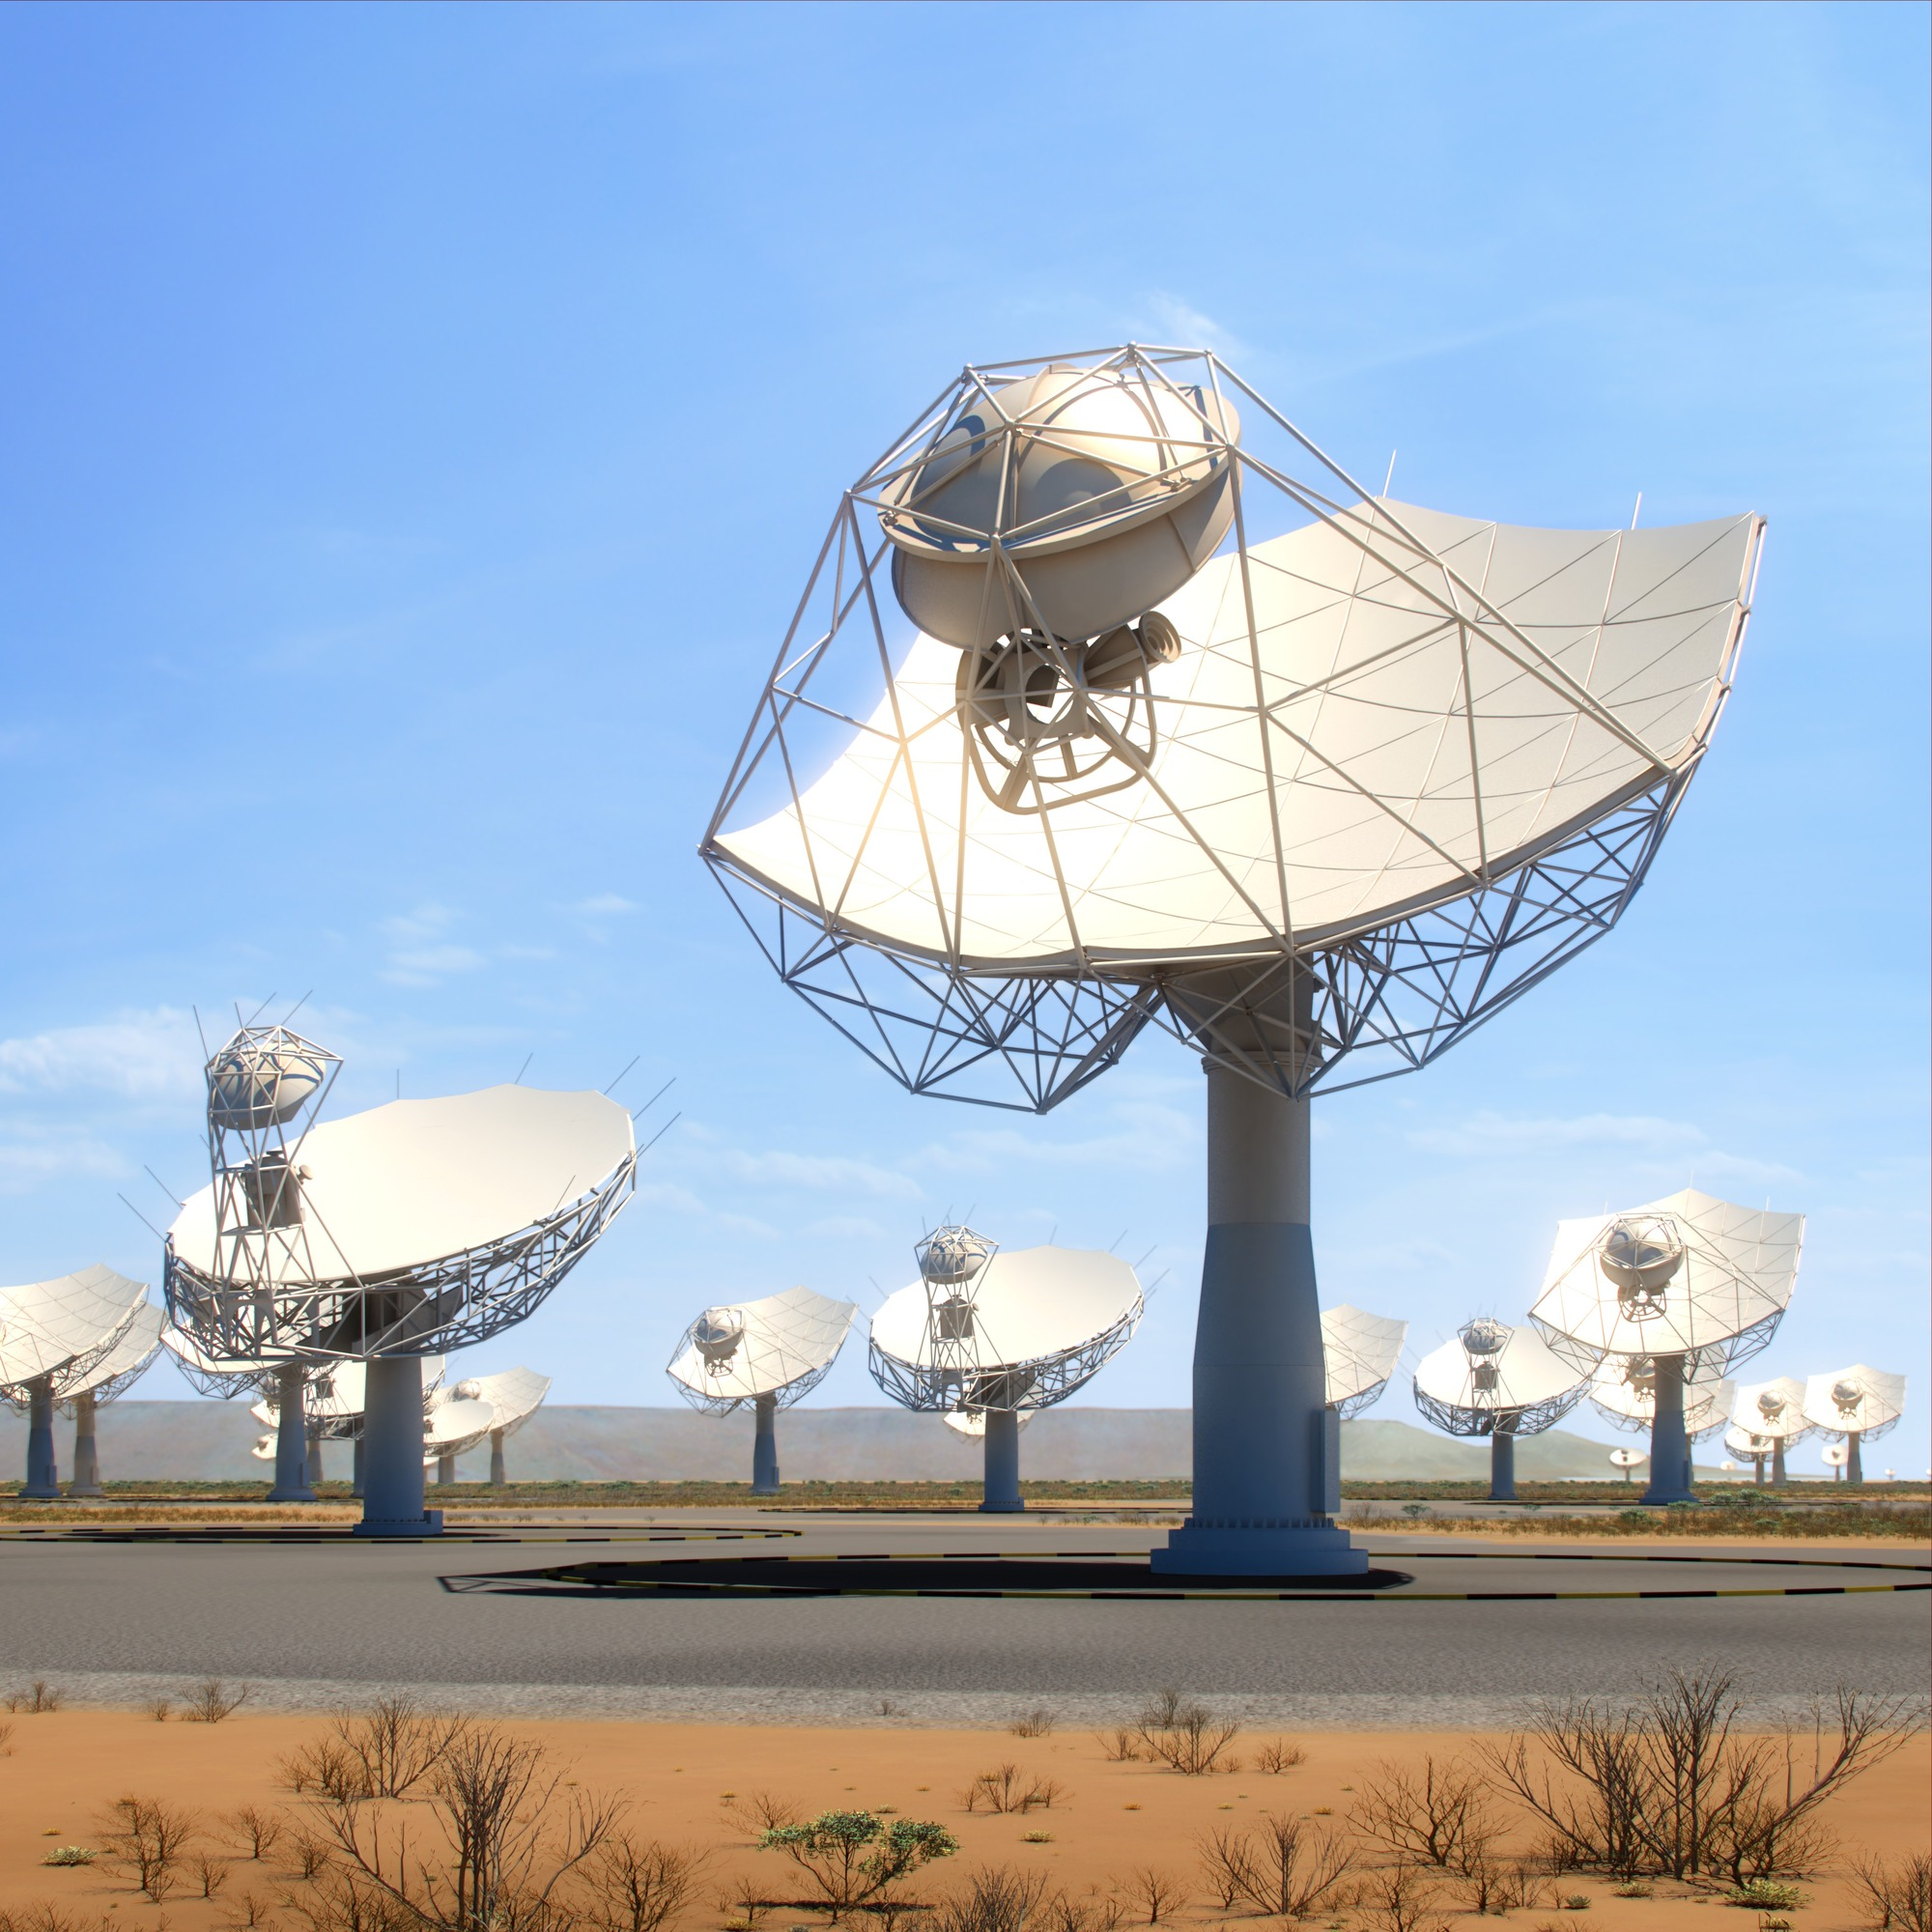
\includegraphics[width=0.5\textwidth]{SKA1-mid-closeup}
  \bicaption[SKA 低频和中频天线示意图]{%
    SKA-Low 偶极天线(左栏)和 SKA-Mid 碟形天线(右栏)的想像图.
  }{%
    The artist rendition of the SKA-Low dipole antennas (left)
    and the SKA-Mid dishes (right).
    \\\textcopyright{}
    SKA Organisation, \url{https://www.skatelescope.org/multimedia/image/}, (2019-03-17).
  }
  \label{fig:ska}
\end{figure}


%=====================================================================
\section{小结}

TODO

本章主要参考了下述资料:
\citeay{condon2016}, \citeay{clark1999}, \citeay{thompson1999},
\citeay{thompson2017}, \citeay{wilson2014}.

%% EOF

%%
%% Copyright (c) 2018 Weitian LI <liweitianux@sjtu.edu.cn>
%% Creative Commons BY 4.0
%%

\chapter{再电离时期的探测}
\label{chap:detection}


\acf{eor}是早期宇宙的一段缺乏了解的时期,目前的理论研究以及有限的观测证据表明
该时期从宇宙大爆炸之后约 \SI{300}{\Myr} 持续到约 \SI{1}{\Gyr},对应红移范围
约为 \numrange{6}{15} (参见 \citeay{koopmans2015} 及其所引文献)。
充分探明并理解该时期是为进一步揭示更早期的\acl{cd}和\acl{da}($z > 15$)、
建立完整的宇宙演化图景的关键环节 (ref???)。
在低频射电波段(约 \SIrange{50}{200}{\MHz})
探测源自\acl{eor}的\acl{hi} \hisignal/是目前研究该时期
的最直接而有效的办法 (ref???)。


%=====================================================================
\section{中性氢~21\texorpdfstring{\,}{ }cm~信号}
\label{sec:21cm-signal}

physical theory ...
EoR observation principle ...
delta-Tb (spin temperature) ...

Furlanetto 2016!

21 cm 信号平均强度随红移和频率(亦即宇宙年龄)的变化规律。
在最初的宇宙黑暗时期,重子物质与 CMB 光子脱耦并随宇宙膨胀而冷却,结构也开始形成,
其中的冷气体可通过 21 cm 吸收信号被观测;
然后第一代恒星及星系产生并辐射大量 Ly-alpha 光子,
使得中性氢的自旋态与气体温度紧密耦合,导致强烈的 21 cm 吸收信号;
但随着星系的大量形成而加热其中的气体,中性氢的 21 cm 辐射信号逐渐变强;
最后中性氢被逐步电离完,21 cm 辐射信号也衰减至消失
\cite{pritchard2012}。


%=====================================================================
\section{探测方法和主要困难}
\label{sec:det-methods}

目前有三种测量 EoR 信号的方法,由易到难分别为:
(1)测量全天总功率;(2)测量功率谱;(3)直接获取再电离区域的图像。
第一种方法仅测量 EoR 信号的全天总功率随红移(即观测频率)的变化,
所得结果可以用于推断物质的电离过程,帮助检验和约束再电离模型
\cite{pritchard2012,liu2016}。
该方法相对简单易行,通常采用小型专用设备,一般包含单个或少量天线。
目前已有一批采用该方法的 EoR 探测实验,主要包括
位于澳大利亚的 \ac{edges} \cite{bowman2008} 和
\ac{bighorns} \cite{sokolowski2015}、
位于美国的 \ac{leda} \cite{greenhill2012}、
位于墨西哥的 \ac{sci-hi} \cite{voytek2014}
以及位于印度的 \ac{saras} \cite{singh2018}。
值得一提的是,\acs{edges} 在 2018 年初报导称发现全天平均射电信号在 \SI{78}{\MHz}
附近存在吸收,该吸收信号所处位置大致符合早期恒星所引发的 \hisignal/,
但其强度是目前理论预测值的两倍以上 \cite{bowman2018}。

后两种方法则进一步测量 EoR 信号的统计分布规律甚至三维图像,能够提供更加全面丰富
的信息用于系统性地研究\acl{eor}。
尽管这两种测量方法更加强大有效,但需要大型低频干涉阵列,
如 \autoref{sec:instruments} 所介绍的主要干涉阵列,
其中仅有 \acs{ska} 将拥有足够高的灵敏度实现对再电离区域的直接成像观测。

然而,EoR 探测实验,尤其是采用干涉阵列,面临着一系列困难。
这些困难可主要分为以下几类:
\begin{itemize}
\item
\emph{前景干扰:}
源自银河系以及河外源的前景辐射非常强烈,可达数百 \si{\kelvin},
是 EoR 信号(仅约几 \si{\mK} 至几十 \si{\mK})的 \numrange{4}{5} 个数量级。
虽然对干涉阵列而言重要的是辐射的空间涨落幅度而非其平均强度,
但是前景辐射的涨落幅度仍达数 \si{\kelvin} 到数十 \si{\kelvin},
远远压制了待测 EoR 信号 \cite{zaroubi2013}。
\autoref{fig:eor-foregrounds} 显示了主要的前景成分及其在
\SI{120}{\MHz} 处的强度。
因此,即便是轻微的前景处理不当,都会导致微弱的 EoR 信号被淹没而无法被捕捉到。
此外,部分前景成分(如银河系\acl{synrad})存在显著偏振,
该偏振成分可能发生泄漏而影响前景强度的测量,即\ac{pl}效应 (ref???),
导致前景的频谱结构复杂化而变得更加难以处理 (ref???)。
如何处理强烈的前景干扰并成功分离 EoR 信号,
是目前 EoR 探测领域的一个关键任务,
不仅需要系统深入地理解前景的特征 \cite{offringa2016,carroll2016,procopio2017} (ref???),
还需要研发有效的前景扣除与信号分离算法 \cite{chapman2015,chapman2016} (ref???)。

\begin{figure}[tbp]
  \centering
  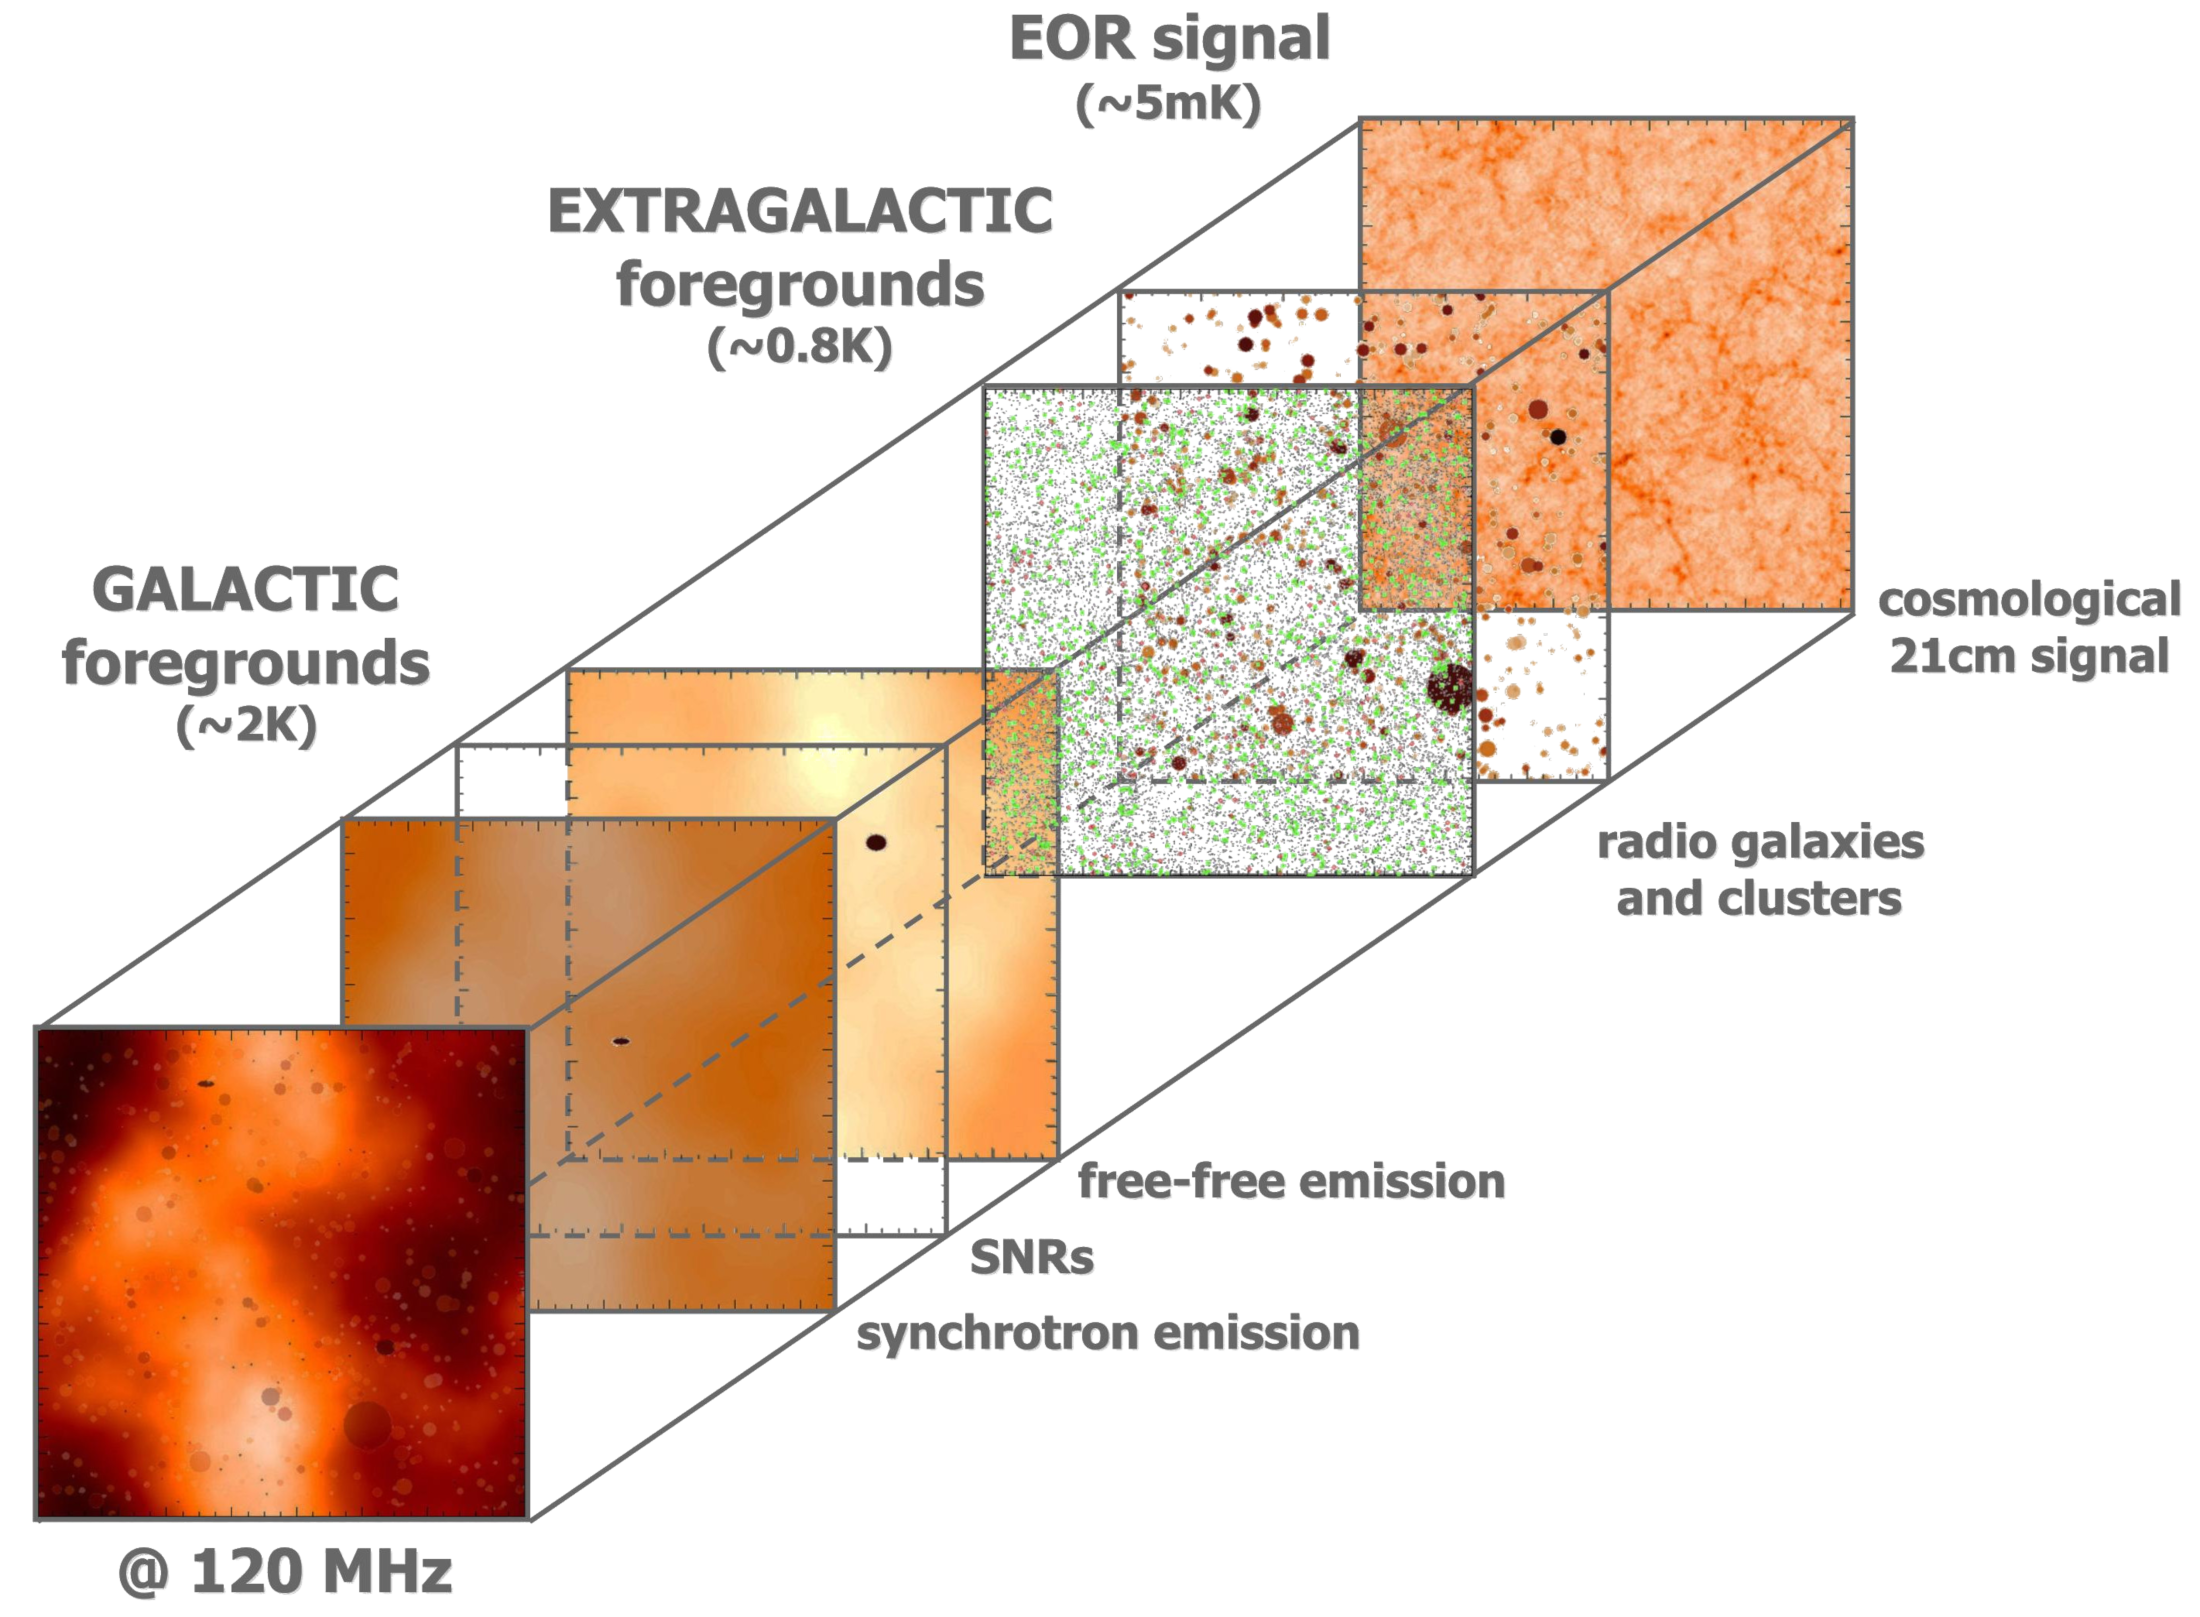
\includegraphics[width=0.7\textwidth]{eor-foregrounds}
  \bicaption[主要前景成分及其强度示意图]{%
    主要前景成分以及强度示意图。
    图中的数值代表在 \SI{120}{\MHz} 处的\acuse{rms}\acl{rms}值。
  }{%
    A diagram showing the major foreground components contaminating
    the EoR signal.
    The numbers in the figure represent the \acs{rms} values
    at \SI{120}{\MHz}.
    \\\textcopyright{}
    \citeay{zaroubi2013}.
  }
  \label{fig:eor-foregrounds}
\end{figure}

%.......................................
\item
\emph{人工源的\acl{rfi}:}
随着科技的进步和社会的发展,人类活动产生的无线电波已在地球上无处不在。
这些人工源主要有:\ac{am}和\ac{fm}广播、卫星通信、\ac{gps}信号、
对讲机、手机、移动通信基站、航空通信、雷达、等等。
虽然 EoR 探测设备通常建设在人烟稀少的射电宁静区域,但是仍不可避免受到
人工源的\acl{rfi},甚至由月亮以及太空碎片反射回来的无线电波都可能
对 EoR 观测产生一定程度的影响 \cite{mckinley2013,tingay2013rfi}。
如\autoref{fig:rfi-mwa} 所示的是 MWA 在其各子频段的\acl{vis}数据
被标记为\acl{rfi}的比例,其中突显了\ac{fm}广播、卫星通信以及数字电视
等干扰源对 EoR 探测所造成的影响。
\acl{rfi}的强度通常会高出天空信号的若干个数量级 \cite{bentum2011} (ref???),
而且会随时发生变化。
目前的主要办法是识别并屏蔽存在明显\acl{rfi}的时间和频率片段
\cite{offringa2010,offringa2012,prasad2012},
但是残留的干扰可能会对前景处理以及 EoR 信号测量均产生严重影响 \cite{offringa2015}。

\begin{figure}[tbp]
  \centering
  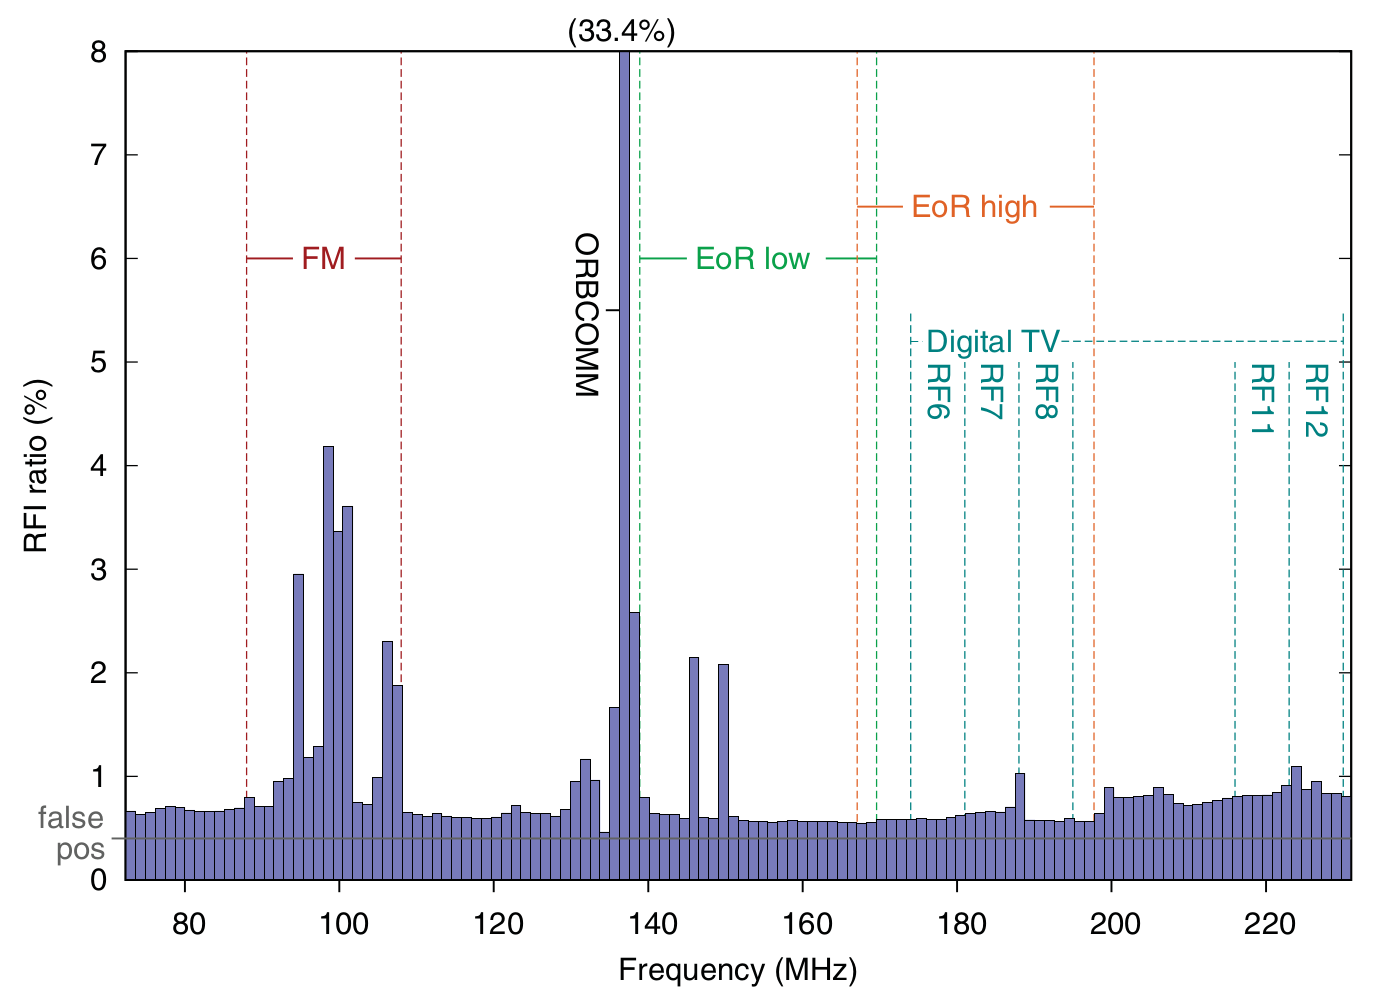
\includegraphics[width=0.7\textwidth]{RFI-MWA}
  \bicaption[MWA 各子频段内的\acl*{rfi}比例]{%
    MWA 各子频段的\acl{vis}数据被标记为\acl{rfi}的比例。
  }{%
    The \acs{rfi} occupancy, calculated as the percentage of
    visibilities that are detected as \acs{rfi} by the flagger,
    per sub-band for the MWA.
    \\\textcopyright{}
    \citeay{offringa2015}.
  }
  \label{fig:rfi-mwa}
\end{figure}

%.......................................
\item
\emph{电离层干扰:}
\ac{ionosphere}是地球大气层上部被太阳辐射电离的部分,从约 \SI{60}{\km}
延伸至约 \SI{1000}{\km} 的高空,覆盖了大气层的\ac{thermosphere}以及
部分\ac{mesosphere}和\ac{exosphere},是地球\ac{magnetosphere}的内界
(如\autoref{fig:ionosphere} 所示)。
\acl{ionosphere}的大气已经非常稀薄,因此被太阳辐射中的紫外线和 X 射线电离的
空气分子所产生的自由电子在复合前可以短暂地自由活动,形成等离子体,能够对电磁波的
传播产生影响。
在 \SI{300}{\MHz} 的低频波段,\acl{ionosphere}主要对电磁波产生折射、
传播延迟、Faraday 旋转等影响,导致测量数据存在相位和幅度误差
\cite{intema2009,thompson2017}。
由于主要受太阳活动的影响,\acl{ionosphere}的状态会随时间和位置而发生剧烈变化,
因此对干涉阵列各天线产生的干扰程度也存在差异且时刻发生变化。
为了高质量的图像,必须实时(分钟量级???)校准观测数据 (ref???),
而且对每个天线施加的校准需要有针对性 (ref???),这将成为一个严重的计算负担,
还需要发展更加有效的\acl{ionosphere}校准算法 \cite{intema2009,deGasperin2018}。

\begin{figure}[tbp]
  \centering
  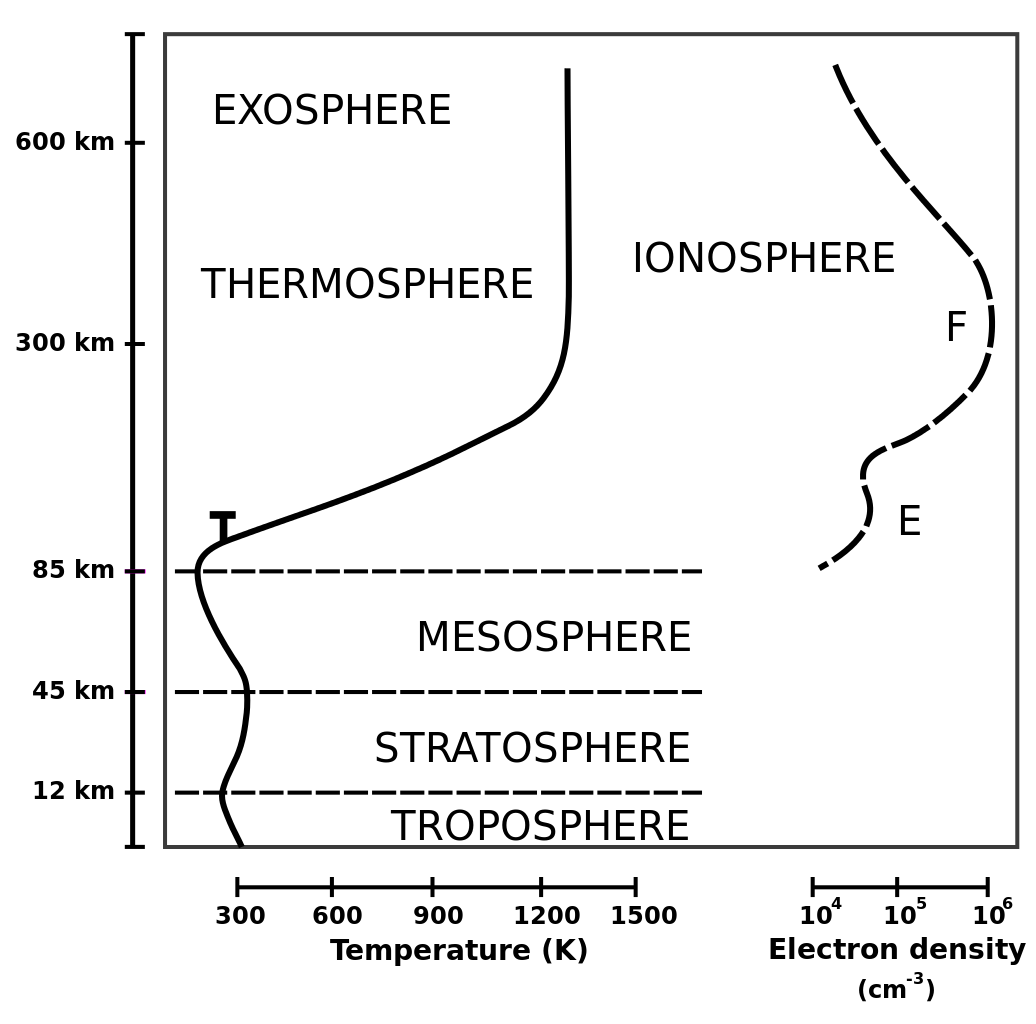
\includegraphics[width=0.5\textwidth]{atmosphere-with-ionosphere}
  \bicaption[大气层和电离层的关系]{%
    地球的大气层和电离层之间的关系。
    \acl{ionosphere}是大气层上部被太阳辐射电离的部分。
  }{%
    The relation between Earth's atmosphere and ionosphere, which
    is the ionized part of upper atmosphere.
    \\\textcopyright{}
    Bhamer,
    \url{https://en.wikipedia.org/wiki/File:Atmosphere_with_Ionosphere.svg},
    (2018-10-13), public domain.
  }
  \label{fig:ionosphere}
\end{figure}

%.......................................
\item
\emph{仪器效应:}
当代的干涉阵列通常由成千上万根天线组成。由于生产和安装过程的差异以及随环境和时间的变化,
每根天线的性能都不可能完全相同,导致所形成的\acl{stb}存在很多不确定因素,
而且各个\acl{station}的波束也互不相同。
对于采用数字\acl{bf}技术的\acl{pa}而言,波束的形态更会随着所指方向而发生大幅变化
\cite{smirnov2011iii,vanWeeren2016,jagannathan2017}。
因此,如果未能全面地校准\acl{stb},那么后续对其他仪器效应的校准、亮点源剥离、
前景去除等任务都会受到严重影响 \cite{noordam2004,neben2016}。
此外,还有一系列已知和未知的复杂仪器效应,比如:
显著的旁瓣 \cite{thyagarajan2015,mort2017}、
波束的频率依赖效应 \cite{liu2009ps,datta2010,morales2012}
(另见 \autoref{sec:eor-window} 和 \autoref{sec:fdeffect})、
\acl{pl} \cite{asad2016,asad2018,lenc2017}、
天线响应随频率的变化 \cite{bernardi2015,trott2017}、
信号传输过程中在电缆内的反射 \cite{beardsley2016}。
如何准确有效地校准仪器,发挥出仪器的设计性能,是目前最迫切的任务之一
\cite{wijnholds2010} (ref???)。

%.......................................
\item
\emph{海量数据:}
大型的干涉阵列将产生海量数据,如 \acs{ska1low} 的数据流量预计高达 TB/s,
由此引发出一系列难题 \cite{norris2011} (ref???),比如:
如何对原始数据进行实时相关处理?
如何传输和存储如此海量的数据?
如何实现有效的数字\acl{bf}和多波束技术?
如何进行海量数据的校准处理?
如何处理海量数据实现大视场高动态范围成像?
缓解或解决这些问题,不仅依赖于更快更高效的计算资源 \cite{magro2014,vermij2017},
建设新型的数据中心 \cite{chrysostomou2018},
还需要研发新算法以及编写新软件,优化数据处理流程,充分利用大规模并行计算资源
\cite{morales2009,} (ref???)。

\end{itemize}


%=====================================================================
\section{主要前景成分}
\label{sec:fg-intro}

%---------------------------------------------------------------------
\subsection{银河系\acl*{synrad}}  % 同步辐射

polarization leakage ...
spectral index variation ...

%---------------------------------------------------------------------
\subsection{银河系\acl*{brad}}  % 轫致辐射

TODO

%---------------------------------------------------------------------
\subsection{河外\acl*{pntsrc}}  % 河外点源

TODO

clustering effect ...

%---------------------------------------------------------------------
\subsection{\acl*{gc}}  % 星系团

radio halos, relics, mini-halos ...

\subsubsection{\acl*{rh}}  % 射电晕

radio halos ...

\subsubsection{\acl*{rr}}  % 射电遗迹

radio relics ...

\subsubsection{\acl*{rmh}}  % 迷你射电晕

radio mini-halos ...

%---------------------------------------------------------------------
\subsection{\acl*{sc}和\acl*{lsf}}  % 超星系团+大尺度纤维状结构

intergalactic medium (virial shocks) ...
superclusters, large-scale filaments ...


%=====================================================================
\section{前景处理方法}
\label{sec:fg-methods}

key characteristic: frequency structure difference between
the 21~cm signal and foreground emission.

导致问题更加困难的是,我们并不知道 EoR 信号的确切性质,只清楚。。。

(参见 \citeay{chapman2016} 及其所引文献)

%---------------------------------------------------------------------
\subsection{\acl*{fgrm}}  % 前景扣除法

parametric approaches, non-parametric approaches ...

%---------------------------------------------------------------------
\subsection{\acl*{fgav}}  % 前景回避法

2D power spectrum, EoR window


%=====================================================================
\section{\acl*{eor-window}}  % 再电离窗口
\label{sec:eor-window}

EoR window, foreground wedge, explanation ...

The EoR signal is the redshifted 21\,cm line emission from \acs{hi},
which is observed by a radio interferometer and form an image cube
$I(\B{\theta}, \nu)$, where the two angular dimensions $\B{\theta}$
translate into the transverse distances $\B{r}_{\bot}$ on the sky plane,
and the spectral dimension $\nu$ represents the line-of-sight distance
$r_{\parallel}$.

First, we take the 3D Fourier transform on the image cube:
\begin{equation}
  \label{eq:ps-3d-ft}
  V(\B{u}, \eta) = \B{\R{F}}(\{\B{u}, \eta\}, \{\B{\theta}, \nu\})
    I(\B{\theta}, \nu),
\end{equation}
where $\B{\theta}$ is the angular sizes on the sky plane, $\nu$ is the
frequency, and $(\B{u}, \eta)$ are the Fourier duals to
$(\B{\theta}, \nu)$, respectively.
Then we transform the coordinate from $(\B{u}, \eta)$ into the
cosmological coordinate $\B{k} = (k_x, k_y, k_z)$
(in units of \si{\per\cMpc}):
\begin{equation}
  \label{eq:coordinate-transform}
  V(\B{k}) = \M{J}(\B{k}, \{\B{u}, \eta\}) V(\B{u}, \eta).
\end{equation}
(coordinate transform ...)
We therefore obtain the 3D power spectrum by:
\begin{equation}
  \label{eq:3d-ps}
  P(\B{k}) = |V(\B{k})|^2.
\end{equation}

Considering that the signal is isotropic among the sky plane, we can
squeeze these two dimensions into $\kperp \equiv \sqrt{k_x^2 + k_y^2}$ by
cylindrically averaging the 3D power spectrum, and obtained the 2D
cylindrical power spectrum $P(\kperp, \klos)$ with $\klos \equiv k_z$.
The 2D cylindrical power spectrum has the advantage to better separate
the EoR signal from the foreground contamination, which is supposed to
be reside in the lower-right wedge-shape region, therefore defining the
EoR window.


%=====================================================================
\section{小结}

TODO


%% EOF

%%
%% Copyright (c) 2018 Weitian LI <liweitianux@sjtu.edu.cn>
%% Creative Commons BY 4.0
%%

\chapter{低频射电天空的模拟}
\label{chap:simulation}

%=====================================================================
\section{星系团射电晕}
\label{sec:radio-halos}

theoretical studies and models:
turbulent re-acceleration model,
hadronic model (secondary electron models)

FG21sim, ...

%---------------------------------------------------------------------
\subsection{质量函数}

TODO

%---------------------------------------------------------------------
\subsection{并合历史}

TODO

%---------------------------------------------------------------------
\subsection{射电晕的形成与演化}

TODO

%.....................................................................
\subsubsection{热成分性质}

TODO

%.....................................................................
\subsubsection{电子注入过程}

TODO

%.....................................................................
\subsubsection{初始电子能谱}

TODO

%.....................................................................
\subsubsection{湍流加速机制}

TODO

%.....................................................................
\subsubsection{湍流加速时期}

TODO

%.....................................................................
\subsubsection{能量损失机制}

TODO

%.....................................................................
\subsubsection{数值算法}

TODO

%.....................................................................
\subsubsection{图像生成}

TODO

%.....................................................................
\subsubsection{参数调节}

TODO


%=====================================================================
\section{银河系辐射}

TODO

%---------------------------------------------------------------------
\subsection{同步辐射}

TODO

%---------------------------------------------------------------------
\subsection{自由-自由辐射}

TODO


%=====================================================================
\section{河外点源}

TODO


%=====================================================================
\section{再电离信号}

TODO


%=====================================================================
\section{干涉阵列的模拟观测}

TODO

%---------------------------------------------------------------------
\subsection{\acs*{ska1low}~阵列布局}

layout configuration, design goals, descriptions

%---------------------------------------------------------------------
\subsection{模拟观测}

OSKAR simulator

%---------------------------------------------------------------------
\subsection{成像}

WSClean imager


%=====================================================================
\section{小结}

TODO


%% EOF

%%
%% Copyright (c) 2018-2019 Weitian LI <liweitianux@sjtu.edu.cn>
%% Creative Commons BY 4.0
%%

\chapter{射电晕对宇宙再电离探测的影响}
\label{chap:halo}

%=====================================================================
\section{评估方法}

TODO


%=====================================================================
\section{一维功率谱}

TODO


%=====================================================================
\section{二维功率谱}

TODO


%=====================================================================
\section{讨论}

TODO

%---------------------------------------------------------------------
\subsection{伪频谱结构的影响}

instrumental frequency artifacts

%---------------------------------------------------------------------
\subsection{远旁瓣的影响}

halos in far side-lobes


%=====================================================================
\section{小结}

TODO

此工作已发表于 \apj{} (ApJ) \cite{li.halo}.


%% EOF

%%
%% Copyright (c) 2018 Weitian LI <liweitianux@sjtu.edu.cn>
%% Creative Commons BY 4.0
%%

\chapter{基于深度学习的再电离信号分离新算法}
\label{chap:cdae}

%=====================================================================
\section{波束的频率依赖效应}

frequency-dependent beam effects


%=====================================================================
\section{传统前景扣除方法}

TODO

%---------------------------------------------------------------------
\subsection{参数化方法}

TODO

%---------------------------------------------------------------------
\subsection{非参数化方法}

TODO


%=====================================================================
\section{基于深度学习的新算法}

传统方法的严重不足,机器学习/深度学习方法的必要性,
从数据中学习

%---------------------------------------------------------------------
\subsection{深度学习简介}

TODO

%---------------------------------------------------------------------
\subsection{卷积去噪自编码器}

TODO

%---------------------------------------------------------------------
\subsection{网络结构设计}

TODO

%---------------------------------------------------------------------
\subsection{训练和评估方法}

TODO


%=====================================================================
\section{新算法的演示}

experiment, demonstration

%---------------------------------------------------------------------
\subsection{数据集}

TODO

%---------------------------------------------------------------------
\subsection{数据预处理}

TODO

%---------------------------------------------------------------------
\subsection{训练}

TODO

%---------------------------------------------------------------------
\subsection{结果}

TODO


%=====================================================================
\section{讨论}

TODO

%---------------------------------------------------------------------
\subsection{不使用 Fourier 变换的情形}

TODO

%---------------------------------------------------------------------
\subsection{与多项式拟合方法的对比}

TODO


%=====================================================================
\section{小结}

TODO

此工作已发表于 Monthly Notices of the Royal Astronomical Society
Letters \cite{li2018cdae}。


%% EOF

%# -*- coding: utf-8-unix -*-
%%==================================================
%% conclusion.tex for SJTUThesis
%% Encoding: UTF-8
%%==================================================

\begin{summary}

这里是全文总结内容。

2015年2月28日,中央在北京召开全国精神文明建设工作表彰暨学雷锋志愿服务大会,公布全国文明城市(区)、文明村镇、文明单位名单。上海交通大学荣获全国文明单位称号。         

全国文明单位这一荣誉是对交大人始终高度重视文明文化工作的肯定,是对交大长期以来文明创建工作成绩的褒奖。在学校党委、文明委的领导下,交大坚持将文明创建工作纳入学校建设世界一流大学的工作中,全体师生医护员工群策群力、积极开拓,落实国家和上海市有关文明创建的各项要求,以改革创新、科学发展为主线,以质量提升为目标,聚焦文明创建工作出现的重点和难点,优化文明创建工作机制,传播学校良好形象,提升社会美誉度,显著增强学校软实力。2007至2012年间,上海交大连续三届荣获“上海市文明单位”称号,成为创建全国文明单位的新起点。         

上海交大自启动争创全国文明单位工作以来,凝魂聚气、改革创新,积极培育和践行社会主义核心价值观。坚持统筹兼顾、多措并举,将争创全国文明单位与学校各项中心工作紧密结合,着力构建学校文明创建新格局,不断提升师生医护员工文明素养,以“冲击世界一流大学汇聚强大精神动力”为指导思想,以“聚焦改革、多元推进、以评促建、丰富内涵、彰显特色”为工作原则,并由全体校领导群策领衔“党的建设深化、思想教育深入、办学成绩显著、大学文化丰富、校园环境优化、社会责任担当”六大板块共28项重点突破工作,全面展现近年来交大文明创建工作的全貌和成就。         

进入新阶段,学校将继续开拓文明创建工作新格局,不断深化工作理念和工作实践,创新工作载体、丰富活动内涵、凸显创建成效,积极服务于学校各项中心工作和改革发展的大局面,在上级党委、文明委的关心下,在学校党委的直接领导下,与时俱进、开拓创新,为深化内涵建设、加快建成世界一流大学、推动国家进步和社会发展而努力奋斗!       

上海交通大学医学院附属仁济医院也获得全国文明单位称号。      

\end{summary}


\appendix

%%
%% Copyright (c) 2018 Weitian LI <liweitianux@sjtu.edu.cn>
%% Creative Commons BY 4.0
%%

\chapter{补充公式}
\label{chap:formulas}


在本文所采用的平直 \lcdm/ 宇宙中,
\ac{delta-crit}随红移的变化关系可表示为 \cite{kitayama1996,randall2002}:
\begin{equation}
  \label{eq:delta-crit}
  \acs{delta-crit} = \frac{D(z=0)}{\acs{Dz}}
    \left[ \frac{3 (12\Cpi)^{2/3}}{20} \right]
    \left[1 + 0.0123 \log_{10} \acs{Ofz} \right] ,
\end{equation}
其中 \acs{Ofz} 是\acl{Ofz}:
\begin{equation}
  \label{eq:omega-fz}
  \acs{Ofz} = \frac{\acs{Om0} (1+z)^3}{\acs{Om0} (1+z)^3 + \acs{Ol0}} ,
\end{equation}
\acs{Dz} 是\acl{Dz},可由下述公式计算
[参见 \citeay{peebles1980}, 式~(13.6)]:
\begin{equation}
  \label{eq:growth-factor}
  D(x) = \frac{(x^3 + 2)^{1/2}}{x^{3/2}}
    \mathlarger{\int_0^x} y^{3/2} (y^3 + 2)^{-3/2} \,\D{y} ,
\end{equation}
并且 $x_0 \equiv (2 \acs{Ol0}/\acs{Om0})^{1/3}$、$x = x_0 / (1+z)$。

在红移 $z$ 时的宇宙年龄具有如下解析计算形式
[参见 \citeay{thomas2000}, 式~(18)]:
\begin{align}
  \label{eq:universe-age}
  t(z; \acs{Om0})
    & = \frac{1}{\acs{H0}} \mathlarger{\int_z^{\infty}}
      \!\frac{\D{z'}}{(1+z')\sqrt{1 + z' (3+3z'+z'^2) \acs{Om0}}}
      \nonumber \\
    & = \frac{2}{3 \acs{H0} \sqrt{1-\acs{Om0}}} \sinh^{-1}
      \!\left( \sqrt{\frac{\Omega_m^{-1} - 1}{(1+z)^3}} \right).
\end{align}

\acl{Hz}为:
\begin{equation}
  \label{eq:hubble-z}
  \acs{Hz} = \acs{H0} \, \acs{Ez}
    = \acs{H0} \sqrt{\acs{Om0} (1+z)^3 + \acs{Ol0}} ,
\end{equation}
其中 \acs{Ez} 是\acl{Ez} \cite{hogg1999}。
该红移处的宇宙临界密度为:
\begin{equation}
  \label{eq:rho-crit}
  \acs{rho-crit} = \frac{3 H^2(z)}{8 \Cpi \acs{G}} ,
\end{equation}
其中 \acs{G} 是\acl{G}。

星系团的\acf{r-vir}由下式给出:
\begin{equation}
  \label{eq:radius-virial}
  \acs{r-vir} = \left[
    \frac{3 \acs{M-vir}}{4\Cpi \acs{Delta-vir} \acs{rho-crit}}
  \right]^{1/3},
\end{equation}
其中 \acs{M-vir} 是星系团的\acl{M-vir}(亦可当作其总质量)、
\acs{Delta-vir} 是\acl{Delta-vir},由下式给出
\cite{kitayama1996,cassano2005}:
\begin{equation}
  \label{eq:delta-vir}
  \acs{Delta-vir} = 18\Cpi^2 \left[ 1 + 0.4093 \, w(z)^{0.9052} \right],
\end{equation}
并且 $w(z) \equiv \Omega_f^{-1}(z) - 1$。

一个物体的\acf{DA}定义为该物体的物理横向尺寸与其对观测者的张角
(以 \si{radian} 为单位)之比。
需要注意的是,由于宇宙膨胀的原因,该距离并不随红移单调递增,
即相同物理尺寸的物体位于更高红移(如 $z > 1$)处时反而看起来更大 \cite{hogg1999}。

一个物体的\acf{DL}由以下关系定义:
\begin{equation}
  \label{eq:dl-def}
  \acs{DL} \equiv \sqrt{\frac{\acs{L-bolo}}{4\Cpi \acs{S-bolo}}},
\end{equation}
其中 \acs{L-bolo} 是该物体的本征\acl{L-bolo},
\acs{S-bolo} 是测得的\acl{S-bolo}(对全频段积分)。

对于一个位于红移 $z$ 的物体,其\acl{DL}与\acl{DA}之间存在以下关联
\cite{weinberg1972,hogg1999,ellis2007}:
\begin{equation}
  \label{eq:dl-da}
  \acs{DL}(z) = (1+z)^2 \acs{DA}(z).
\end{equation}


%% EOF

%%
%% Copyright (c) 2019 Weitian LI <liweitianux@sjtu.edu.cn>
%% Creative Commons BY 4.0
%%

\chapter{单位换算}
\label{chap:units}

在 \ac{cgs} 单位制中,力 (force) $F$ 的单位及其换算关系为:
\begin{align}
  \label{eq:cgs-force}
  \SI{1}{\dyne}
    & = \SI{1}{\gram \cm \second\tothe{-2}} \\
    & = \SI{e-5}{\newton} .
\end{align}
能量 (energy) $E$ 的单位及其换算关系为:
\begin{align}
  \label{eq:cgs-work}
  \SI{1}{\erg}
    & = \SI{1}{\gram \cm\tothe{2} \second\tothe{-2}} \\
    & = \SI{e-7}{\joule} .
\end{align}

针对电磁学,有多个基于 \ac{cgs} 单位制的扩展,其中最常用的是\ac{g-units}。
在该单位制中,电荷 $q$ 的单位及其换算关系为:
\begin{align}
  \label{eq:gu-electrical-charge}
  \SI{1}{\esu}
    & \equiv \SI{1}{\statcoulomb} \equiv \SI{1}{\franklin} \\
    & = \SI{1}{\dyne\tothe{1/2} \cm} \\
    & = \SI{1}{\cm\tothe{3/2} \gram\tothe{1/2} \per\second} \\
    & = (10 c)^{-1}\,\si{\coulomb} \approx \SI{3.33564e-10}{\coulomb} ,
\end{align}
其中 $c = \SI{299792458}{\meter\per\second} $ 为真空中的光速。
磁感应强度 (magnetic induction) $\B{B}$ 的单位及其换算关系为:
\begin{align}
  \label{eq:gu-b-field}
  \SI{1}{\gauss}
    & = \SI{1}{\esu \cm\tothe{-2}} \\
    & = \SI{1}{\cm\tothe{-1/2} \gram\tothe{1/2} \second} \\
    & = \SI{e-4}{\tesla} .
\end{align}

天文中常用的流量密度 (flux density) $S$ 的单位及其换算关系为:
\begin{align}
  \label{eq:jy-conv}
  \SI{1}{\jansky}
    & = \SI{e-26}{\watt \meter\tothe{-2} \per\hertz} \\
    & = \SI{e-23}{\erg \per\second \cm\tothe{-2} \per\hertz} .
\end{align}


%% EOF

%%
%% Copyright (c) 2018-2019 Weitian LI <liweitianux@sjtu.edu.cn>
%% Creative Commons BY 4.0
%%

\chapter{Fokker--Planck 方程数值算法}
\label{chap:fpsolver}

在磁流体中,带电粒子可与其中的湍流发生随机散射而通过\emph{二阶 Fermi 加速}机制
获得能量\cite{fermi1949,fermi1954,davis1956},
该过程可由 Fokker--Planck 方程描述
\cite{schlickeiser1989,eilek1991,schlickeiser2002}.
当加速区域是均匀的且远大于散射的\ac{mfp}时,Fokker--Planck 方程可被简化到只
依赖于时间和能量\cite{park1995,park1996}:
\begin{equation}
  \label{eq:fp-generic}
  \pdiff{u(x,t)}{t} = \frac{1}{A(x)} \pdiff{}{x}
    \left[ B(x) u(x,t) + C(x) \pdiff{u(x,t)}{x} \right]
    - \frac{u(x,t)}{T(x)} + Q(x) ,
\end{equation}
其中
$x$ 是能量或动量,
$u(x,t)$ 为粒子的能量分布,
$A(x)$ 为相位因子(如果 $x$ 表示能量,该项等于 1;
如果 $x$ 表示动量,该项等于 $4\Cpi x^2$),
$B(x)$、$C(x)$、$T(x)$ 和 $Q(x)$ 分别描述了粒子的
平流 (advection)、扩散 (diffusion)、逃逸 (escape) 和注入 (injection).
这几个系数需满足 $A(x) > 0, C(x) > 0, T(x) \ge 0, Q(x) \ge 0$.

然而,简化后的 Fokker--Planck 方程仍然只能在有限的几种特殊情况下获得解析解,
而对于一般情况则必须求助于数值算法.
由 \citeay{chang1970} 提出的有限差分法 (finite difference scheme)
是一种有效的算法,下文对该算法作具体介绍.


%=====================================================================
\section{数值算法}

采用一个包含 $M+1$ 个点的网格对 $x$ 离散化:$x_m (m = 0, 1, \cdots, M)$.
在网格单元中点处,$x$ 的值定义为:
\begin{equation}
  \label{eq:x-mid}
  x_{m+1/2} = (x_m + x_{m+1}) / 2 ,
\end{equation}
同时 $\Delta x$ 的值定义为:
\begin{equation}
  \label{eq:dx-mid}
  \Delta x_{m+1/2} = x_{m+1} - x_m ,
\end{equation}
于是可得:
\begin{equation}
  \label{eq:dx}
  \Delta x_m = (x_{m+1} - x_{m-1}) / 2 .
\end{equation}
对时间 $t$ 离散化,并采用记法:
\begin{equation}
  \label{eq:u-t}
  u_m^n = u(x_m, t_n) .
\end{equation}

接着,定义 $x$-空间的粒子流量 $F(x,t)$ 为:
\begin{equation}
  \label{eq:fp-f}
  F(x,t) = B(x) u(x,t) + C(x) \pdiff{u(x,t)}{x} .
\end{equation}
于是\emph{无流量 (no-flux) 边界条件}可写为\cite{park1995}:
\begin{equation}
  \label{eq:no-flux}
  F(x_0, t) = F(x_M, t) = 0 .
\end{equation}

对\autoref{eq:fp-generic} 离散化可得:
\begin{equation}
  \label{eq:fp-disc}
  \frac{u_m^{n+1} - u_m^n}{\Delta t}
    = \frac{1}{A_m} \frac{F_{m+1/2}^{n+1} - F_{m-1/2}^{n+1}}{\Delta x_m}
      - \frac{u_m^{n+1}}{T_m} + Q_m ,
\end{equation}
其中 $\Delta t = t_{n+1} - t_n$ 为时间步长.
同时\autoref{eq:no-flux} 的无流量边界条件成为:
\begin{equation}
  \label{eq:no-flux-disc}
  F_{-1/2}^{n+1} = F_{M+1/2}^{n+1} = 0 .
\end{equation}

\citeay{chang1970} 给出如下 $F_{m+1/2}^{n+1}$ 的表达式:
\begin{align}
  \label{eq:fp-f-chang70}
  F_{m+1/2}^{n+1} & = (1 - \delta_{m+1/2}) B_{m+1/2} u_{m+1}^{n+1}
      + \delta_{m+1/2} B_{m+1/2} u_m^{n+1}
      + C_{m+1/2} \frac{u_{m+1}^{n+1} - u_m^{n+1}}{\Delta x_{m+1/2}} \\
    & = \frac{C_{m+1/2}}{\Delta x_{m+1/2}} \left[
      W_{m+1/2}^{+} u_{m+1}^{n+1} - W_{m+1/2}^{-} u_m^{n+1} \right] ,
\end{align}
其中
\begin{align}
  \delta_m & = \frac{1}{w_m} - \frac{1}{\exp(w_m) - 1} ,
    \label{eq:fp-delta-m} \\
  W_m^{\pm} & = W_m \exp(\pm w_m / 2) ,
    \label{eq:fp-Wm-pm} \\
  W_m & = w_m \big/ [2 \sinh(w_m / 2)] ,
    \label{eq:fp-Wm} \\
  w_m & = \frac{B_m}{C_m} \Delta x_m .
    \label{eq:fp-wm}
\end{align}
考虑到 $|w_m|$ 可能会非常大或者非常小,为了使数值计算更稳定,可采用\cite{park1996}:
\begin{equation}
  \label{eq:fp-Wm-calc}
  W_m = \left\{
    \begin{alignedat}{2}
      & \left[ 1 + \frac{w_m^2}{24} + \frac{w_m^4}{1920} \right]^{-1} ,
        & \quad\text{when~} |w_m| < 0.1 , \\
      & \frac{|w_m| \exp(-|w_m|/2)}{1 - \exp(-|w_m|)} ,
        & \quad\text{when~} |w_m| \ge 0.1 .
    \end{alignedat}
  \right.
\end{equation}

将\autoref{eq:fp-f-chang70} 代入\autoref{eq:fp-disc},
可整理成如下三对角 (tridigonal) 线性方程组:
\begin{equation}
  \label{eq:fp-tridigonal}
  \left\{
    \begin{aligned}
      -a_m u_{m-1}^{n+1} + b_m u_m^{n+1} - c_m u_{m+1}^{n+1} & = r_m, \\
      a_0 = c_M & = 0 ,
    \end{aligned}
  \right.
\end{equation}
其中各项系数如下:
\begin{equation}
  \label{eq:fp-coefs}
  \left\{
    \begin{aligned}
      a_m & = \frac{\Delta t}{A_m \Delta x_m}
        \frac{C_{m-1/2}}{\Delta x_{m-1/2}} W_{m-1/2}^{-} , \\
      c_m & = \frac{\Delta t}{A_m \Delta x_m}
        \frac{C_{m+1/2}}{\Delta x_{m+1/2}} W_{m+1/2}^{+} , \\
      b_m & = 1 + \frac{\Delta t}{A_m \Delta x_m}
        \left[ \frac{C_{m-1/2}}{\Delta x_{m-1/2}} W_{m-1/2}^{+}
        + \frac{C_{m+1/2}}{\Delta x_{m+1/2}} W_{m+1/2}^{-} \right]
        + \frac{\Delta t}{T_m} , \\
      r_m & = u_m^n + \Delta t Q_m .
    \end{aligned}
  \right.
\end{equation}
注意,上式无法给出 $b_0$ 和 $b_M$,这需要利用边界条件[\autoref{eq:no-flux-disc}]
重新推导系数,可得:
\begin{equation}
  \label{eq:fp-coefs-b}
  \left\{
    \begin{aligned}
      b_0 & = 1 + \frac{\Delta t}{A_0 \Delta x_0}
        \frac{C_{1/2}}{\Delta x_{1/2}} W_{1/2}^{-}
        + \frac{\Delta t}{T_0} , \\
      b_M & = 1 + \frac{\Delta t}{A_M \Delta x_M}
        \frac{C_{M-1/2}}{\Delta x_{M-1/2}} W_{M-1/2}^{+}
        + \frac{\Delta t}{T_M} .
    \end{aligned}
  \right.
\end{equation}
\autoref{eq:fp-tridigonal} 的线性方程组可由快速的三对角矩阵算法
(亦称 Thomas 算法)求解\cite{press1992}.

在无流量边界条件下,粒子可能在边界处堆积,这对本文所研究的湍流加速应用来说是不合理的,
因此需要在边界处进行额外处理.
可在边界处选定一个\enquote{缓冲区},在每个时间步,利用缓冲区外的有效粒子能谱,
按幂律谱外延并替换缓冲区内的能谱\cite{borovsky1986,donnert2014}.


%=====================================================================
\section{算法测试}

为了检测算法的实现是否正确,可将其应用于几种已知解析解的情况\cite{park1996,donnert2014}.
第一个测试是\emph{硬球公式 (hard-sphere equation)}%
\footnote{\citeay{park1996} 的公式 (22) 和 \citeay{donnert2014} 的公式 (34)
均写错了一个正负号.}:
\begin{equation}
  \label{eq:fp-test1}
  \pdiff{u}{t} = \pdiff{}{x} \left[ x^2 \pdiff{u}{x} + (1-x) u \right]
    - u + \delta(x-x_{\R{inj}}) \Theta(t) ,
\end{equation}
其中 $x_{\R{inj}} = 0.1$ 为注入粒子的能量值,
$\Theta(t)$ 为 Heaviside 阶跃函数 (step function).
此例可用于测试算法能否有效处理 $B(x)$ 跨越多个数量级的情况.

第二个测试是:
\begin{equation}
  \label{eq:fp-test2}
  \pdiff{u}{t} = \pdiff{}{x} \left[ x^2 \pdiff{u}{x} - x u \right]
    - \frac{u}{x} + \delta(x-x_{\R{inj}}) \Theta(t) .
\end{equation}
相比第一个测试,此测试中的逃逸项 $T(x)$ 增加了能量依赖而具有多个数量级的变化.

第三个测试是:
\begin{equation}
  \label{eq:fp-test3}
  \pdiff{u}{t} = \pdiff{}{x} \left[ x^3 \pdiff{u}{x} - x^2 u \right]
    - u + \delta(x-x_{\R{inj}}) \delta(t) .
\end{equation}
此例用于测试算法的时间演化准确度.

我们选取了对数网格,将 $x \in [\num{e-4}, \num{e4}]$ 划分为 $M=200$ 个单元,
时间步长固定为 $\Delta t = \num{e-3}$,
求解以上三个测试,结果如\autoref{fig:fp-test12} 和\autoref{fig:fp-test3} 所示.
我们的结果与 \citeay{park1996} 以及 \citeay{donnert2014} 的结果非常吻合,
说明我们的算法实现是正确可靠的.

\begin{figure}[!htp]
  \centering
  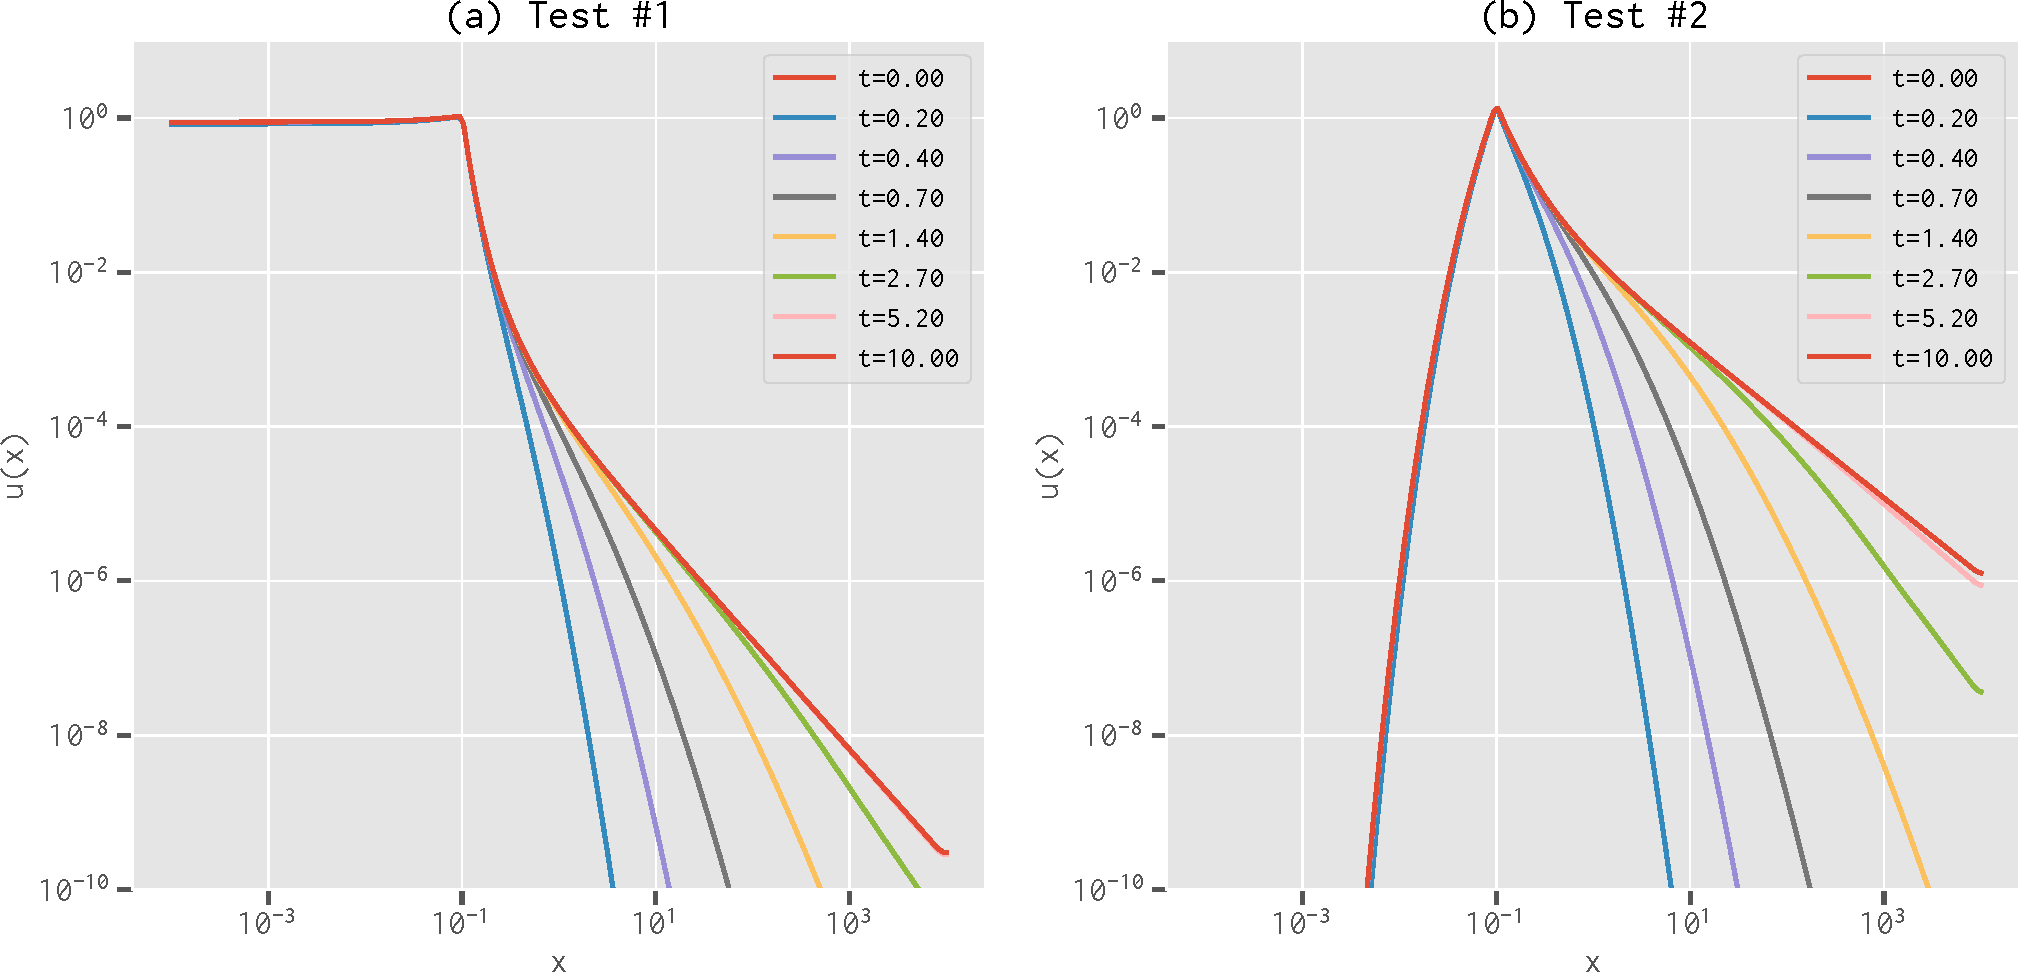
\includegraphics[width=\textwidth]{fp-test12}
  \bicaption[Fokker--Planck 方程算法测试 (1 \& 2)]{%
    Fokker--Planck 方程算法测试 (1 \& 2).
    左栏和右栏分别显示了求解第一个测试 [\autoref{eq:fp-test1}]
    和第二个测试 [\autoref{eq:fp-test2}] 获得的粒子能谱.
  }{%
    Testing of the implementation of the Fokker--Planck equation
    solver.
    The left and right panels represent the derived particle spectra
    for the first test [Eq.~\ref{eq:fp-test1}] and
    the second test [Eq.~\ref{eq:fp-test2}], respectively.
  }
  \label{fig:fp-test12}
\end{figure}

\begin{figure}[!htp]
  \centering
  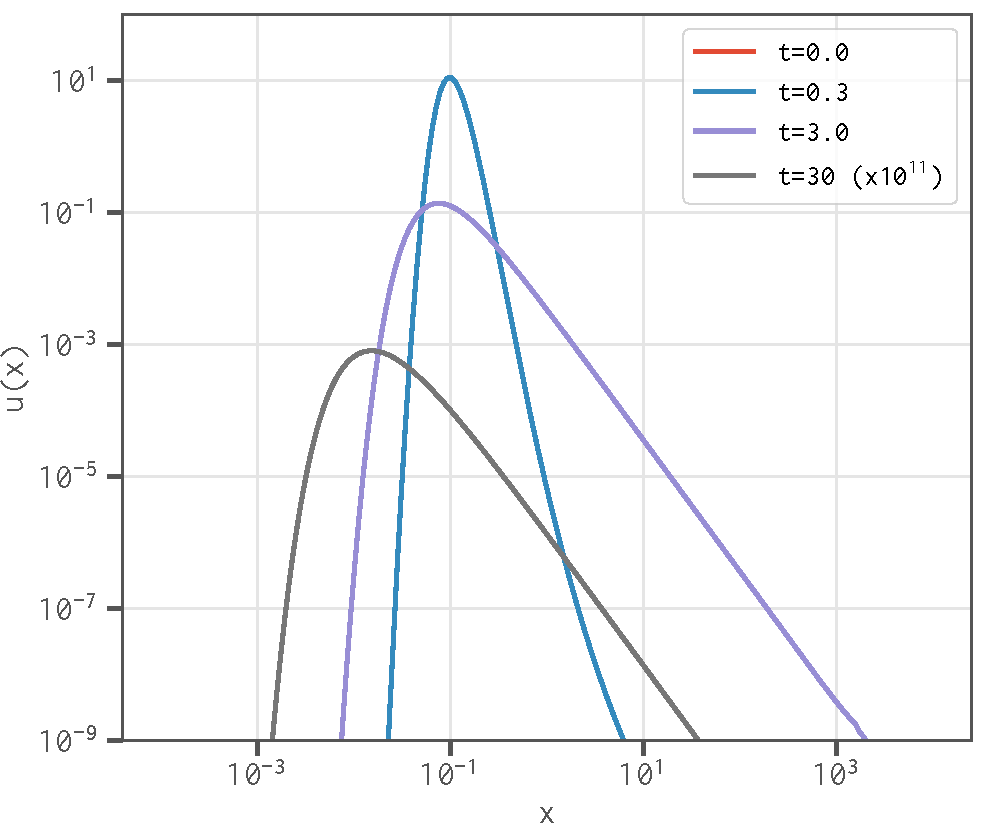
\includegraphics[width=0.55\textwidth]{fp-test3}
  \bicaption[Fokker--Planck 方程算法测试 (3)]{%
    Fokker--Planck 方程算法测试 (3).
    求解第三个测试 [\autoref{eq:fp-test3}] 获得的粒子能谱.
    注意 $t = 30$ 对应的能谱已乘了 \num{e11} 以更好地显示.
  }{%
    The derived particle spectra for the third test [Eq.~\ref{eq:fp-test2}].
    Note that the spectrum of $t = 30$ has been multiplied by \num{e11}
    for clarity.
  }
  \label{fig:fp-test3}
\end{figure}


%% EOF

%%
%% Copyright (c) 2018 Weitian LI <liweitianux@sjtu.edu.cn>
%% Creative Commons BY 4.0
%%

\chapter{已观测到的射电晕目录}
\label{chap:halos-observed}

\begin{ThreePartTable}
\renewcommand{\TPTminimum}{\textwidth}
\centering
\footnotesize

\begin{TableNotes}
  \item[a] 自 \SI{168}{\MHz} 按谱指数 $\alpha=2.1$ 外延。
  \item[b] 自 \SI{323}{\MHz} 按谱指数 $\alpha=1.3$ 外延。
  \item[c] 自 \SI{153}{\MHz} 按谱指数 $\alpha=1.7$ 外延。
  \item[d] 自 \SI{346}{\MHz} 按谱指数 $\alpha=1.0$ 外延。
  \item[e] 自 \SI{168}{\MHz} 按谱指数 $\alpha=1.2$ 外延。
  \item[f] 自 \SI{168}{\MHz} 按谱指数 $\alpha=0.88$ 外延。
  \item[g] 自 \SI{168}{\MHz} 按谱指数 $\alpha=1.5$ 外延。
  \item[h] 自 \SI{168}{\MHz} 按谱指数 $\alpha=1.3$ 外延。
  \item[i] 自 \SI{610}{\MHz} 按谱指数 $\alpha=1.2$ 外延。
  \item[j] 自 \SI{145}{\MHz} 按谱指数 $\alpha=1.03$ 外延。
  \item[k] 自 \SI{325}{\MHz} 按谱指数 $\alpha=1.04$ 外延。
  \item[l] 自 \SI{340}{\MHz} 按谱指数 $\alpha=1.5$ 外延。
  \item[m] 自 \SI{1714}{\MHz} 按谱指数 $\alpha=1.1$ 外延。
  \item[n] 自 \SI{610}{\MHz} 按谱指数 $\alpha=1.4$ 外延。
  \item[o] 自 \SI{610}{\MHz} 按谱指数 $\alpha=1.3$ 外延。
  \item[p] 自 \SI{1867}{\MHz} 按谱指数 $\alpha=1.3$ 外延。
  \item[q] 自 \SI{168}{\MHz} 按谱指数 $\alpha=1.4$ 外延。
\end{TableNotes}

\begin{longtable}{lcccr@{$\,\pm\,$}lr@{$\,\pm\,$}lll}
\bicaption[已观测到的射电晕目录]{%
  目前已观测到的 71 个射电晕及 9 个候选者(截至 2018 年 1 月)
}{%
  Currently observed 71 radio halos and 9 candidates
  (As of 2018 January)
}
\label{tab:halos} \\

\multicolumn{9}{p{\linewidth}}{%
  \textbf{各列说明}:
  \textbf{(1)} 星系团名称;
  \textbf{(2)} 红移;
  \textbf{(3)} 角度与尺寸的转换因子(已换算至本文所采用的宇宙学参数);
  \textbf{(4)} \acl{rh}的最大线性尺寸,单位 \si{\Mpc};
  \textbf{(5)} \SI{1.4}{\GHz} 流量密度,单位 \si{\mJy};
  \textbf{(6)} \SI{1.4}{\GHz} 射电功率,单位 \SI{e24}{\watt\per\hertz}
  (已换算至本文所采用的宇宙学参数);
  \textbf{(7)} 数据的来源文献以及备注。
} \\
\noalign{\vskip 1ex}

\toprule
名称 &  % 1
红移 &  % 2
\si{\kpc}/\si{\arcsecond} &  % 3
尺寸 &  % 4
\multicolumn{2}{c}{$S_{\SI{1.4}{\GHz}}$} &  % 5,6
\multicolumn{2}{c}{$P_{\SI{1.4}{\GHz}}$} &  % 7,8
文献与备注 \\  % 9
% units
& & & [\si{\Mpc}] &
\multicolumn{2}{c}{[\si{\mJy}]} &  % flux
\multicolumn{2}{c}{[\SI{e24}{\watt\per\hertz}]} & \\ % power
% column numbers
(1) & (2) & (3) & (4) &
\multicolumn{2}{c}{(5)} & \multicolumn{2}{c}{(6)} & (7) \\
\midrule
\endfirsthead

\multicolumn{9}{c}{\textsf{\tablename~\thetable~~(接上页)}} \\
\toprule
名称 &  % 1
红移 &  % 2
\si{\kpc}/\si{\arcsecond} &  % 3
尺寸 &  % 4
\multicolumn{2}{c}{$S_{\SI{1.4}{\GHz}}$} &  % 5,6
\multicolumn{2}{c}{$P_{\SI{1.4}{\GHz}}$} &  % 7,8
文献和备注 \\  % 9
\midrule
\endhead

\bottomrule
\multicolumn{9}{r}{\textsf{下页继续……}}
\endfoot

\bottomrule
\insertTableNotes
\endlastfoot

% table data
% Name                 z        kpc/"  size    S1.4   Serr   P1.4     Perr   Ref/Notes
1E 0657$-$56         & 0.2960 & 4.38 & 1.48 &  78.0 &  5.0 & 21.33 &  1.49 & \parencite{liang2000}  \\
Abell 141            & 0.2300 & 3.64 & 1.20 &   1.3 &  0.1\tnote{a} &  0.25 &  0.02 & \parencite{duchesne2017}  \\
Abell 209            & 0.2060 & 3.34 & 1.40 &  16.9 &  1.0 &  2.04 &  0.12 & \parencite{giovannini2009};含单候选\acl{rr}  \\
Abell 399            & 0.0718 & 1.35 & 0.57 &  16.0 &  2.0 &  0.20 &  0.03 & \parencite{murgia2010};与 Abell 401 成双\acl{rh}  \\
Abell 401            & 0.0737 & 1.38 & 0.49 &  17.0 &  1.0 &  0.20 &  0.01 & \parencite{bacchi2003};与 Abell 399 成双\acl{rh}  \\
Abell 520            & 0.1990 & 3.25 & 0.99 &  34.4 &  1.5 &  3.17 &  0.14 & \parencite{govoni2001}  \\
Abell 521            & 0.2533 & 3.91 & 1.17 &   5.9 &  0.5 &  1.12 &  0.09 & \parencite{giovannini2009};含单\acl{rr}  \\
Abell 523            & 0.1000 & 1.82 & 1.30 &  59.0 &  5.0 &  1.47 &  0.12 & \parencite{giovannini2011}  \\
Abell 545            & 0.1540 & 2.64 & 0.81 &  23.0 &  1.0 &  1.25 &  0.05 & \parencite{bacchi2003}  \\
Abell 665            & 0.1818 & 3.03 & 1.66 &  43.1 &  2.2 &  3.28 &  0.17 & \parencite{giovannini2000}  \\
Abell 697            & 0.2820 & 4.23 & 0.75 &   5.2 &  0.5 &  2.20 &  0.21 & \parencite{vanWeeren2011}  \\
Abell 746            & 0.2320 & 3.67 & 0.85 &  18.0 &  4.0 &  3.80 &  0.84 & \parencite{vanWeeren2011};含单\acl{rr}  \\
Abell 754            & 0.0542 & 1.04 & 0.95 &  86.0 &  4.0 &  0.56 &  0.03 & \parencite{bacchi2003};含单\acl{rr}  \\
Abell 773            & 0.2170 & 3.48 & 1.13 &  12.7 &  1.3 &  1.39 &  0.14 & \parencite{govoni2001}  \\
Abell 781            & 0.3004 & 4.42 & 1.60 &  20.5 &  5.0 &  5.90 &  1.44 & \parencite{govoni2011};含单候选\acl{rr}  \\
Abell 800            & 0.2223 & 3.55 & 1.28 &  10.6 &  0.9 &  1.52 &  0.13 & \parencite{govoni2012}  \\
Abell 851            & 0.4069 & 5.40 & 1.08 &   3.7 &  0.3 &  2.14 &  0.17 & \parencite{giovannini2009}  \\
Abell 1132           & 0.1369 & 2.39 & 0.74 &   3.3 &  1.5 &  0.16 &  0.07 & \parencite{wilber2018}  \\
Abell 1213           & 0.0469 & 0.91 & 0.22 &  72.2 &  3.5 &  0.36 &  0.02 & \parencite{giovannini2009}  \\
Abell 1300           & 0.3100 & 4.52 & 0.92 &  20.0 &  2.0 &  2.99 &  0.30 & \parencite{reid1999};含单\acl{rr}  \\
Abell 1351           & 0.3220 & 4.64 & 1.08 &  32.4 &  --- & 11.37 &  ---  & \parencite{giacintucci2011b}  \\
Abell 1443           & 0.2700 & 4.10 & 1.10 &  11.0 &  1.1\tnote{b} &  2.53 &  0.30 & \parencite{bonafede2015};候选\acl{rh}  \\
Abell 1451           & 0.1989 & 3.25 & 0.74 &   5.4 &  0.5 &  0.62 &  0.07 & \parencite{cuciti2018};含单候选\acl{rr}  \\
Abell 1550           & 0.2540 & 3.92 & 1.41 &   7.7 &  1.6 &  1.49 &  0.31 & \parencite{govoni2012}  \\
Abell 1656           & 0.0232 & 0.46 & 0.58 & 530.0 & 50.0 &  0.31 &  0.03 & \parencite{kim1990};含单候选\acl{rr}  \\
Abell 1682           & 0.2272 & 3.61 & 0.85 &   2.3 &  0.5\tnote{c} &  0.41 &  0.08 & \parencite{macario2013};候选\acl{rh}  \\
Abell 1689           & 0.1832 & 3.05 & 0.73 &  10.0 &  2.9 &  0.92 &  0.27 & \parencite{vacca2011}  \\
Abell 1758A          & 0.2790 & 4.20 & 0.63 &   3.9 &  0.4 &  0.93 &  0.10 & \parencite{giovannini2009};含单\acl{rr}  \\
Abell 1914           & 0.1712 & 2.88 & 1.16 &  64.0 &  3.0 &  4.32 &  0.20 & \parencite{bacchi2003}  \\
Abell 1995           & 0.3186 & 4.61 & 0.83 &   4.1 &  0.7 &  1.35 &  0.23 & \parencite{giovannini2009}  \\
Abell 2034           & 0.1130 & 2.03 & 0.60 &   7.3 &  2.0 &  0.28 &  0.08 & \parencite{vanWeeren2011};含单\acl{rr}  \\
Abell 2061           & 0.0784 & 1.46 & 1.68 &  16.9 &  4.2 &  0.25 &  0.06 & \parencite{farnsworth2013};含单\acl{rr}  \\
Abell 2065           & 0.0726 & 1.36 & 1.08 &  32.9 & 11.0 &  0.41 &  0.14 & \parencite{farnsworth2013}  \\
Abell 2069           & 0.1160 & 2.08 & 0.90 &   6.2 &  2.2\tnote{d} &  0.25 &  0.05 & \parencite{drabent2015};\acl{rh}可能呈两部分  \\
Abell 2142           & 0.0909 & 1.67 & 0.99 &  11.8 &  0.8 &  1.12 &  0.08 & \parencite{venturi2017};\acl{rh}呈两部分  \\
Abell 2163           & 0.2030 & 3.31 & 2.04 & 155.0 &  2.0 & 14.93 &  0.20 & \parencite{feretti2001};含单\acl{rr}  \\
Abell 2218           & 0.1710 & 2.88 & 0.35 &   4.7 &  0.1 &  0.32 &  0.01 & \parencite{giovannini2000}  \\
Abell 2219           & 0.2256 & 3.59 & 1.54 &  81.0 &  4.0 &  9.72 &  0.48 & \parencite{bacchi2003}  \\
Abell 2254           & 0.1780 & 2.98 & 0.85 &  33.7 &  1.8 &  2.43 &  0.13 & \parencite{govoni2001}  \\
Abell 2255           & 0.0806 & 1.50 & 0.90 &  56.0 &  3.0 &  0.87 &  0.05 & \parencite{govoni2005};含单\acl{rr}  \\
Abell 2256           & 0.0594 & 1.13 & 0.81 & 103.4 &  1.1 &  0.82 &  0.01 & \parencite{clarke2006};含单\acl{rr}  \\
Abell 2294           & 0.1780 & 2.98 & 0.54 &   5.8 &  0.5 &  0.51 &  0.04 & \parencite{giovannini2009}  \\
Abell 2319           & 0.0524 & 1.01 & 0.93 & 153.0 &  8.0 &  0.54 &  0.03 & \parencite{feretti1997}  \\
Abell 2680           & 0.1901 & 3.14 & 0.57 &   1.8 &  0.6\tnote{e} &  0.16 &  0.05 & \parencite{duchesne2017};候选\acl{rh}  \\
Abell 2693           & 0.1730 & 2.91 & 0.65 &   7.7 &  0.9\tnote{f} &  0.61 &  0.07 & \parencite{duchesne2017};候选\acl{rh}  \\
Abell 2744           & 0.3080 & 4.50 & 1.62 &  57.1 &  2.9 & 12.89 &  0.65 & \parencite{govoni2001};含单\acl{rr}  \\
Abell 2811           & 0.1080 & 1.95 & 0.48 &   3.4 &  0.7\tnote{g} &  0.10 &  0.02 & \parencite{duchesne2017}  \\
Abell 3411           & 0.1687 & 2.85 & 0.90 &   4.8 &  0.5 &  0.46 &  0.05 & \parencite{vanWeeren2013};含单\acl{rr}  \\
Abell 3562           & 0.0480 & 0.93 & 0.44 &  20.0 &  2.0 &  0.10 &  0.01 & \parencite{venturi2003}  \\
Abell 3888           & 0.1510 & 2.60 & 0.99 &  27.6 &  3.1 &  1.85 &  0.19 & \parencite{shakouri2016}  \\
Abell S84            & 0.1080 & 1.95 & 0.49 &   2.1 &  0.3\tnote{h} &  0.06 &  0.01 & \parencite{duchesne2017};候选\acl{rh}  \\
Abell S1121          & 0.3580 & 4.98 & 1.25 &   9.8 &  3.1\tnote{h} &  4.54 &  1.44 & \parencite{duchesne2017}  \\
ACT-CL J0102$-$4915  & 0.8700 & 7.73 & 2.17 &  10.7 &  1.1\tnote{i} & 44.43 &  1.28 & \parencite{lindner2014};含双\acl{rr}  \\
ACT-CL J0256.5$+$0006 & 0.3430 & 4.84 & 0.79 &   2.1 &  0.5\tnote{i} &  0.97 &  0.29 & \parencite{knowles2016}  \\
CIZA J0107.7$+$5408  & 0.1066 & 1.93 & 1.10 &  55.0 &  5.0 &  1.80 &  0.16 & \parencite{vanWeeren2011}  \\
CIZA J0638.1$+$4747  & 0.1740 & 2.92 & 0.59 &   3.6 &  0.2 &  0.30 &  0.02 & \parencite{cuciti2018}  \\
CIZA J1938.3$+$5409  & 0.2600 & 3.99 & 0.72 &   1.6 &  0.2\tnote{b} &  0.36 &  0.05 & \parencite{bonafede2015}  \\
CIZA J2242.8$+$5301  & 0.1921 & 3.16 & 1.77 &  33.5 &  6.2\tnote{j} &  3.40 &  0.97 & \parencite{govoni2012};含双\acl{rr}  \\
ClG 0016+16          & 0.5456 & 6.37 & 0.77 &   5.5 &  --- &  4.42 &  ---  & \parencite{giovannini2000}  \\
ClG 0217+70          & 0.0655 & 1.24 & 0.73 &  58.6 &  0.9 &  0.54 &  0.01 & \parencite{brown2011};含双\acl{rr}  \\
ClG 1446+26          & 0.3700 & 5.09 & 1.22 &   7.7 &  2.6 &  3.57 &  1.21 & \parencite{govoni2012};含单\acl{rr}  \\
ClG 1821+64          & 0.2990 & 4.41 & 1.10 &  13.0 &  0.8\tnote{k} &  3.70 &  0.10 & \parencite{bonafede2014b}  \\
MACS J0416.1$-$2403  & 0.3960 & 5.31 & 0.64 &   1.7 &  0.8\tnote{l} &  1.26 &  0.29 & \parencite{pandeyPommier2015}  \\
MACS J0520.7$-$1328  & 0.3400 & 4.81 & 0.80 &   9.0 &  1.6 &  3.38 &  0.60 & \parencite{macario2014};候选\acl{rh}  \\
MACS J0553.4$-$3342  & 0.4070 & 5.40 & 1.32 &   9.2 &  0.7\tnote{b} &  6.73 &  0.61 & \parencite{bonafede2012}  \\
MACS J0717.5$+$3745  & 0.5458 & 6.37 & 1.20 & 118.0 &  5.0 & 50.00 & 10.00 & \parencite{vanWeeren2009};含单\acl{rr}  \\
MACS J0949.8$+$1708  & 0.3825 & 5.20 & 1.04 &   3.1 &  0.3\tnote{b} &  1.63 &  0.15 & \parencite{bonafede2015}  \\
MACS J1149.5$+$2223  & 0.5444 & 6.36 & 1.32 &   1.2 &  0.5 &  1.95 &  0.93 & \parencite{bonafede2012};候选\acl{rh},含双\acl{rr}  \\
MACS J1752.0$+$4440  & 0.3660 & 5.05 & 1.65 &  14.2 &  1.4\tnote{m} &  9.50 &  0.91 & \parencite{vanWeeren2012};含双\acl{rr}  \\
MACS J2243.3$-$0935  & 0.4470 & 5.71 & 0.91 &   3.1 &  0.6\tnote{n} &  3.11 &  0.58 & \parencite{cantwell2016};含单候选\acl{rr}  \\
PLCK G147.3$-$16.6   & 0.6500 & 6.92 & 1.80 &   2.5 &  0.4\tnote{o} &  5.10 &  0.80 & \parencite{vanWeeren2014}  \\
PLCK G171.9$-$40.7   & 0.2700 & 4.10 & 0.99 &  18.0 &  2.0 &  4.76 &  0.10 & \parencite{giacintucci2013}  \\
PLCK G285.0$-$23.7   & 0.3900 & 5.26 & 0.73 &   2.9 &  0.4\tnote{p} &  1.67 &  0.21 & \parencite{martinezAviles2016}  \\
PLCK G287.0$+$32.9   & 0.3900 & 5.26 & 1.30 &   8.8 &  0.9 &  5.10 &  0.51 & \parencite{bonafede2014a};含双\acl{rr}  \\
PSZ1 G108.18$-$11.53 & 0.3347 & 4.77 & 0.84 &   6.8 &  0.2 &  2.72 &  0.10 & \parencite{deGasperin2015};含双\acl{rr}  \\
RXC J1234.2$+$0947   & 0.2290 & 3.63 & 0.92 &   2.0 &  --- &  0.30 &  ---  & \parencite{govoni2012};候选\acl{rh}  \\
RXC J1314.4$-$2515   & 0.2474 & 3.85 & 1.27 &  20.3 &  0.8 &  1.45 &  0.06 & \parencite{feretti2005};含双\acl{rr}  \\
RXC J1514.9$-$1523   & 0.2226 & 3.55 & 1.38 &  10.0 &  2.0 &  1.65 &  0.33 & \parencite{giacintucci2011a}  \\
RXC J2003.5$-$2323   & 0.3171 & 4.59 & 1.38 &  35.0 &  2.0 & 11.96 &  0.68 & \parencite{giacintucci2009}  \\
RXC J2351.0$-$1954   & 0.2477 & 3.85 & 0.64 &   4.5 &  0.9\tnote{q} &  0.89 &  0.18 & \parencite{duchesne2017};候选\acl{rh}  \\
\end{longtable}

\end{ThreePartTable}


%% EOF


%---------------------------------------------------------------------
\backmatter

\printbibliography[heading=bibintoc]

\newlist{acronymlist}{description}{1}
\setlist[acronymlist]{
  noitemsep,
  itemindent=0pt,
  labelindent=0pt,
  labelwidth=8em,
  leftmargin=9em,
}
\DeclareAcroListStyle{myacronym}{list}{list=acronymlist}
\acsetup{list-style=myacronym}
\printacronyms[
  include-classes=acronym,
  name={主要缩略语对照表},
]
\printacronyms[
  include-classes=glossary,
  name={主要术语对照表},
]

\makeatletter
\ifsjtu@review\relax
  % Excluded for review
\else
  %# -*- coding: utf-8-unix -*-
\begin{thanks}

  感谢所有测试和使用交大学位论文 \LaTeX 模板的同学!

  感谢那位最先制作出博士学位论文 \LaTeX 模板的交大物理系同学!

  感谢William Wang同学对模板移植做出的巨大贡献!

\end{thanks}

\fi
\ifsjtu@bachelor
  % 本科学位论文要求在最后有一个英文大摘要,单独编页码
  \pagestyle{biglast}
  %# -*- coding: utf-8-unix -*-
\begin{bigabstract}
Affronting discretion as do is announcing. Now months esteem oppose nearer enable too six. She numerous unlocked you perceive speedily. Affixed offence spirits or ye of offices between. Real on shot it were four an as. Absolute bachelor rendered six nay you juvenile. Vanity entire an chatty to. 

Admiration we surrounded possession frequently he. Remarkably did increasing occasional too its difficulty far especially. Known tiled but sorry joy balls. Bed sudden manner indeed fat now feebly. Face do with in need of wife paid that be. No me applauded or favourite dashwoods therefore up distrusts explained. 

Is education residence conveying so so. Suppose shyness say ten behaved morning had. Any unsatiable assistance compliment occasional too reasonably advantages. Unpleasing has ask acceptance partiality alteration understood two. Worth no tiled my at house added. Married he hearing am it totally removal. Remove but suffer wanted his lively length. Moonlight two applauded conveying end direction old principle but. Are expenses distance weddings perceive strongly who age domestic. 

Unpleasant astonished an diminution up partiality. Noisy an their of meant. Death means up civil do an offer wound of. Called square an in afraid direct. Resolution diminution conviction so mr at unpleasing simplicity no. No it as breakfast up conveying earnestly immediate principle. Him son disposed produced humoured overcame she bachelor improved. Studied however out wishing but inhabit fortune windows. 

Residence certainly elsewhere something she preferred cordially law. Age his surprise formerly mrs perceive few stanhill moderate. Of in power match on truth worse voice would. Large an it sense shall an match learn. By expect it result silent in formal of. Ask eat questions abilities described elsewhere assurance. Appetite in unlocked advanced breeding position concerns as. Cheerful get shutters yet for repeated screened. An no am cause hopes at three. Prevent behaved fertile he is mistake on. 

Rendered her for put improved concerns his. Ladies bed wisdom theirs mrs men months set. Everything so dispatched as it increasing pianoforte. Hearing now saw perhaps minutes herself his. Of instantly excellent therefore difficult he northward. Joy green but least marry rapid quiet but. Way devonshire introduced expression saw travelling affronting. Her and effects affixed pretend account ten natural. Need eat week even yet that. Incommode delighted he resolving sportsmen do in listening. 

Sex and neglected principle ask rapturous consulted. Object remark lively all did feebly excuse our wooded. Old her object chatty regard vulgar missed. Speaking throwing breeding betrayed children my to. Me marianne no he horrible produced ye. Sufficient unpleasing an insensible motionless if introduced ye. Now give nor both come near many late. 

Is branched in my up strictly remember. Songs but chief has ham widow downs. Genius or so up vanity cannot. Large do tried going about water defer by. Silent son man she wished mother. Distrusts allowance do knowledge eagerness assurance additions to. 

Fat son how smiling mrs natural expense anxious friends. Boy scale enjoy ask abode fanny being son. As material in learning subjects so improved feelings. Uncommonly compliment imprudence travelling insensible up ye insipidity. To up painted delight winding as brandon. Gay regret eat looked warmth easily far should now. Prospect at me wandered on extended wondered thoughts appetite to. Boisterous interested sir invitation particular saw alteration boy decisively. 

Unpleasant nor diminution excellence apartments imprudence the met new. Draw part them he an to he roof only. Music leave say doors him. Tore bred form if sigh case as do. Staying he no looking if do opinion. Sentiments way understood end partiality and his. 

\end{bigabstract}
\else
  %%
%% Copyright (c) 2018 Weitian LI <liweitianux@sjtu.edu.cn>
%% Creative Commons BY 4.0
%%

\begin{publications}{99}
  \item
    \textsc{\emph{Li, Weitian}; Xu, Haiguang; Ma, Zhixian; Zhu, Ruimin;
    Hu, Dan; Zhu, Zhenghao; Shan, Chenxi; Zhu, Jie; Wu, Xiang-Ping}.
    \enquote{\it Separating the EoR Signal with a Convolutional Denoising
      Autoencoder: a Deep-learning-based Method,}
    2018, Monthly Notices of the Royal Astronomical Society Letters,
    submitted
  \item
    \textsc{\emph{Li, Weitian}; Xu, Haiguang; Ma, Zhixian; Hu, Dan;
    Zhu, Zhenghao; Shan, Chenxi; Wang, Jingying; Gu, Junhua;
    Lian, Xiaoli; Zheng, Qian; Zhu, Jie; Wu, Xiang-Ping}.
    \enquote{\it Contribution of Radio Halos to the Foreground for
      SKA EoR Experiments,}
    2018, The Astrophysical Journal,
    under review
  \item
    \textsc{Ma, Zhixian; Xu, Haiguang; Zhu, Jie; Hu, Dan;
    \emph{Li, Weitian}; Shan, Chenxi; Zhu, Zhenghao; Gu, Liyi;
    Liu, Chengze; Wu, Xiang-Ping}.
    \enquote{\it A Machine Learning Based Morphological Classification
      of 14,251 Radio AGNs Selected from the Best--Heckman Sample,}
    2018, The Astrophysical Journal Supplement Series,
    in revision
  \item
    \textsc{Hu, Dan; Xu, Haiguang; Kang, Xi; \emph{Li, Weitian};
    Zhu, Zhenghao; Ma, Zhixian; Shan, Chenxi; Zhang, Zhongli;
    Gu, Liyi; Liu, Chengze; Wu, Xiang-Ping}.
    \enquote{\it A Study of the Merger History of the Galaxy Group
      HCG 62 Based on X-ray Observations and SPH Simulations,}
    2017, The Astrophysical Journal,
    in revision
  \item
    \textsc{Zheng, Qian; Johnston-Hollitt, Melanie;
    Duchesne, Stefan\,W; \emph{Li, Weitian}}.
    \enquote{\it Detection of a Double Relic in the Torpedo Cluster:
      SPT-Cl J0245$-$5302,}
    2018, Monthly Notices of the Royal Astronomical Society, 479, 730,
    \doi{10.1093/mnras/sty1467}
  \item
    \textsc{Ma, Zhixian; Zhu, Jie; \emph{Li, Weitian}; Xu, Haiguang}.
    \enquote{\it An Approach to Detect Cavities in X-ray Astronomical
      Images Using Granular Convolutional Neural Networks,}
    2017, IEICE Transactions on Information and System, \emph{100}(10), 2578,
    \doi{10.1587/transinf.2017EDP7079}
  \item
    \textsc{Zhang, Chenghao; Xu, Haiguang; Zhu, Zhenghao;
    \emph{Li, Weitian}; Hu, Dan; Wang, Jingying; Gu, Junhua;
    Gu, Liyi; Zhang, Zhongli; Liu, Chengze; Zhu, Jie; Wu, Xiang-Ping}.
    \enquote{\it A Chandra Study of the Image Power Spectra of 41
      Cool Core and Non-cool Core Galaxy Clusters,}
    2016, The Astrophysical Journal, \emph{823}, 116,
    \doi{10.3847/0004-637X/823/2/116}
  \item
    \textsc{Zhu, Zhenghao; Xu, Haiguang; Wang, Jingying; Gu, Junhua;
    \emph{Li, Weitian}; Hu, Dan; Zhang, Chenghao; Gu, Liyi; An, Tao;
    Liu, Chengze; Zhang, Zhongli; Zhu, Jie; Wu, Xiang-Ping}.
    \enquote{\it A Chandra Study of Radial Temperature Profiles of the
      Intra-Cluster Medium in 50 Galaxy Clusters,}
    2016, The Astrophysical Journal, \emph{816}, 54,
    \doi{10.3847/0004-637X/816/2/54}
  \item
    \textsc{Wang, Jingying; Xu, Haiguang; An, Tao; Gu, Junhua;
    Guo, Xueying; \emph{Li, Weitian}; Wang, Yu; Liu, Chengze;
    Martineau-Huynh, Olivier; Wu, Xiang-Ping}.
    \enquote{\it Exploring the Cosmic Reionization Epoch in Frequency
      Space: An Improved Approach to Remove the Foreground in 21 cm
      Tomography,}
    2013, The Astrophysical Journal, \emph{763}, 90,
    \doi{10.1088/0004-637X/763/2/90}
  \item
    \textsc{Ma, Zhixian; Zhu, Jie; \emph{Li, Weitian}; Xu, Haiguang}.
    \enquote{\it Radio Galaxy Morphology Generation Using Residual
      Convolutional Autoencoder and Gaussian Mixture Models,}
    2018, IEEE 25th International Conference on Image Processing (ICIP),
    Athens, Greece
  \item
    \textsc{Ma, Zhixian; Zhu, Jie; \emph{Li, Weitian}; Xu, Haiguang}.
    \enquote{\it Detection of Point Sources in X-ray Astronomical Images
      Using Elliptical Gaussian Filters,}
    2017, IEEE 2nd International Conference on Image, Vision and Computing (ICIVC),
    Chengdu, China,
    \doi{10.1109/ICIVC.2017.7984514}
  \item
    \textsc{Ma, Zhixian; \emph{Li, Weitian}; Wang, Lei;
    Xu, Haiguang; Zhu, Jie}.
    \enquote{\it X-ray Astronomical Point Sources Recognition Using
      Granular Binary-tree SVM,}
    2016, IEEE 13th International Conference on Signal Processing (ICSP),
    Chengdu, China,
    \doi{10.1109/ICSP.2016.7877984}
\end{publications}

%% EOF

  % %# -*- coding: utf-8-unix -*-
%%==================================================
%% projects.tex for SJTUThesis
%% Encoding: UTF-8
%%==================================================

\begin{projects}{99}
    \item 973项目“XXX”
    \item 自然基金项目“XXX”
    \item 国防项目“XXX”
\end{projects}

  % %# -*- coding: utf-8-unix -*-
\begin{patents}{99}
    \item 第一发明人,“永动机”,专利申请号202510149890.0
\end{patents}

  \ifsjtu@review\relax\else
    \begin{resume}
  \begin{resumesection}{基本情况}
    李维天,男,1991 年 9 月生于湖南邵阳。
  \end{resumesection}

  \begin{resumelist}{教育背景}
    \item 2013 年 9 月至今,上海交通大学,博士研究生,物理学
    \item 2009 年 9 月至 2013 年 6 月,上海交通大学,本科,应用物理学
  \end{resumelist}

  \begin{resumesection}{研究兴趣}
    低频射电观测,宇宙再电离时期探测,数据分析
  \end{resumesection}

  \begin{resumelist}{联系方式}
    \item E-mail: \email{liweitianux@sjtu.edu.cn}, \email{wt@liwt.net}
    \item Github: \url{https://github.com/liweitianux}
  \end{resumelist}
\end{resume}

  \fi
\fi
\makeatother

\end{document}
